\documentclass[]{usiinfbachelorproject}
\usepackage{float}
\captionsetup{labelfont={bf}}

\author{Paolo Aurecchia}

\title{Web-based Visualization of GitHub Repositories}
\subtitle{}
\versiondate{\today}
\begin{committee}
%With more than 1 advisor an error is raised...: only 1 advisor is allowed!
\advisor[Universit\`a della Svizzera Italiana, Switzerland]{Prof.}{Michele}{Lanza}
%You can comment out  these lines if you don't have any assistant
\assistant[Universit\`a della Svizzera Italiana, Switzerland]{Dr.}{Andrea}{Mocci}
\end{committee}


\abstract {
GitHub is a Git repository hosting service that allows users to collaborate on projects and share them with others, using the standard Git commands or with GitHub's user-friendly GUI.
Its basic accounts are free, and they allow users to create public repositories that are readable and downloadable by anyone.
It is currently the largest open-source hosting service, with more than 35 million repositories, which makes it a very interesting and vast source of open-source code.

There already exist tools that are aimed at visualizing repositories, but most of them are not web-based, and they often focus on the statistics of the repositories more than their actual code.
The goal of this project is to build a web application that, given a GitHub repository, produces a 3D representation of the system, portraying information about the system's structure and history of development in a useful and understandable way.
The application would then be usable by anyone who wants to know more about the structure and evolution of his code -- or someone else's code -- hosted on GitHub, with the ease of use of a web application.

The representation of the repository is done through the metaphor of the city, where buildings represent classes, and their details like shape, position and color are mapped to specific metrics of the classes, like their number of methods or fields.
The application also allows to see the different versions of the history of the repository, and it allows to generate videos that show the evolution of the system through time.

To generate the 3D visualizations there are some non-trivial aspects that are taken into consideration.
We looked into which parts and metrics of a class are important and are worth showing in the visualization, while also deciding how these characteristics of the classes have to be mapped to the city.
To position the buildings and the districts in the city in a meaningul and efficent way we developed a rectangle-packing algorithm that reduces the wasted space while maintaining the hierarchical structure of the classes and the packages, and also taking into consideration how they have evolved through time.
We also focused on making sure that the 3D representation is performing well -- and appealing -- when we have thousands of packages or classes to visualize.
}



\begin{document}
\maketitle

\tableofcontents
\pagebreak

%%%%%%%%%%%%%%%%%%%%%%%%%
\section{Introduction} \label{introduction}
%%%%%%%%%%%%%%%%%%%%%%%%%

% \subsection{Motivation} \label{Motivation}
GitHub is the largest open-source hosting service, currently having more than 35 million repositories. Its repositories grow bigger and bigger, and their code gets more complicated and harder to analyze and visualize without the help of specialized software. In the past years there have already been people that created software to visualize different kinds of systems, in both 2D and 3D \cite{Wett07b} \cite{Wett2008b} \cite{Wett2008a}, but they were all desktop applications that were made to be run on the users' computers.

Lately, though, there has been a growth in the development of web applications, both because the interest in web-based application has grown and because the capabilities and the performance of the web browsers themselves have greatly increased, to the point where we can now produce the aforementioned graphical representations using web applications.

\subsection{Goal} \label{Goal}
Our goal is to build an application, WebCity, that is aimed at visualizing Java GitHub repositories in a similar fashion to what had been done in the past \cite{Wett07b} \cite{Wett2008b} \cite{Wett2008a}, but this time with the application being a web application instead of a normal desktop software. This allows the users to use the software without having to download it or set it up, but by simply utilizing the application through their web browser.
WebCity aims at offering more than just a static visualization of the Java repositories. The visualizations are enhanced by various features, such as 3D navigation, interaction with the elements of the visualization, the choice of which versions of the repository we want to see, and a video generating feature that allows to download videos that show the evolution of the systems by concatenating screenshots of the different versions of the system in a single video.

\subsection{Project Description} \label{Project Description}
Our application, WebCity, analyzes public Java repositories hosted on GitHub, parses the code, and produces a 3D representation of the system in a way that resembles a city, where the packages of the Java code are represented by the districts of the city, and the classes are the buildings.

The structure of the city itself depends on the code's metrics. Parameters like the height, the width, and the color of the buildings are mapped to different code metrics, giving information to the user about the system in a visual and interactive way.

The application will not only parse the latest version of the repository, but it will also parse its previous versions, therefore allowing the user to choose which version to visualize and to go through the history of the system. This possibility of changing between the versions of a repository can be seen as a fourth dimension, the time, that allows us to better represent the structure of the system and to convey more information to the user, without having to make the 3D representation itself more complicated.

The visualization will be both navigable and interactive. We will be able to move freely across all the three dimensions, while also having the possibility to interact with the different elements on screen with different features, like displaying information of the elements we are hovering, tagging functionalities, a querying function to look for specific classes or packages, and a video generation feature that allows to generate a video whose frames are represented by the different versions of the system.\\\\\\\\

\textbf{An example.} Figure \ref{fig:example} shows a version of the repository of ArgoUML that can be found on GitHub, visualized through WebCity. We can see how the classes have different appearances, depending on their metrics.

We can also notice how some portions of the visualization appear empty: that is because those portions are areas reserved for packages and classes that are not visible at the moment, because they do not exist in this specific version: they could have been deleted, moved or they simply haven't been created yet.
\begin{figure} [H]
\centering
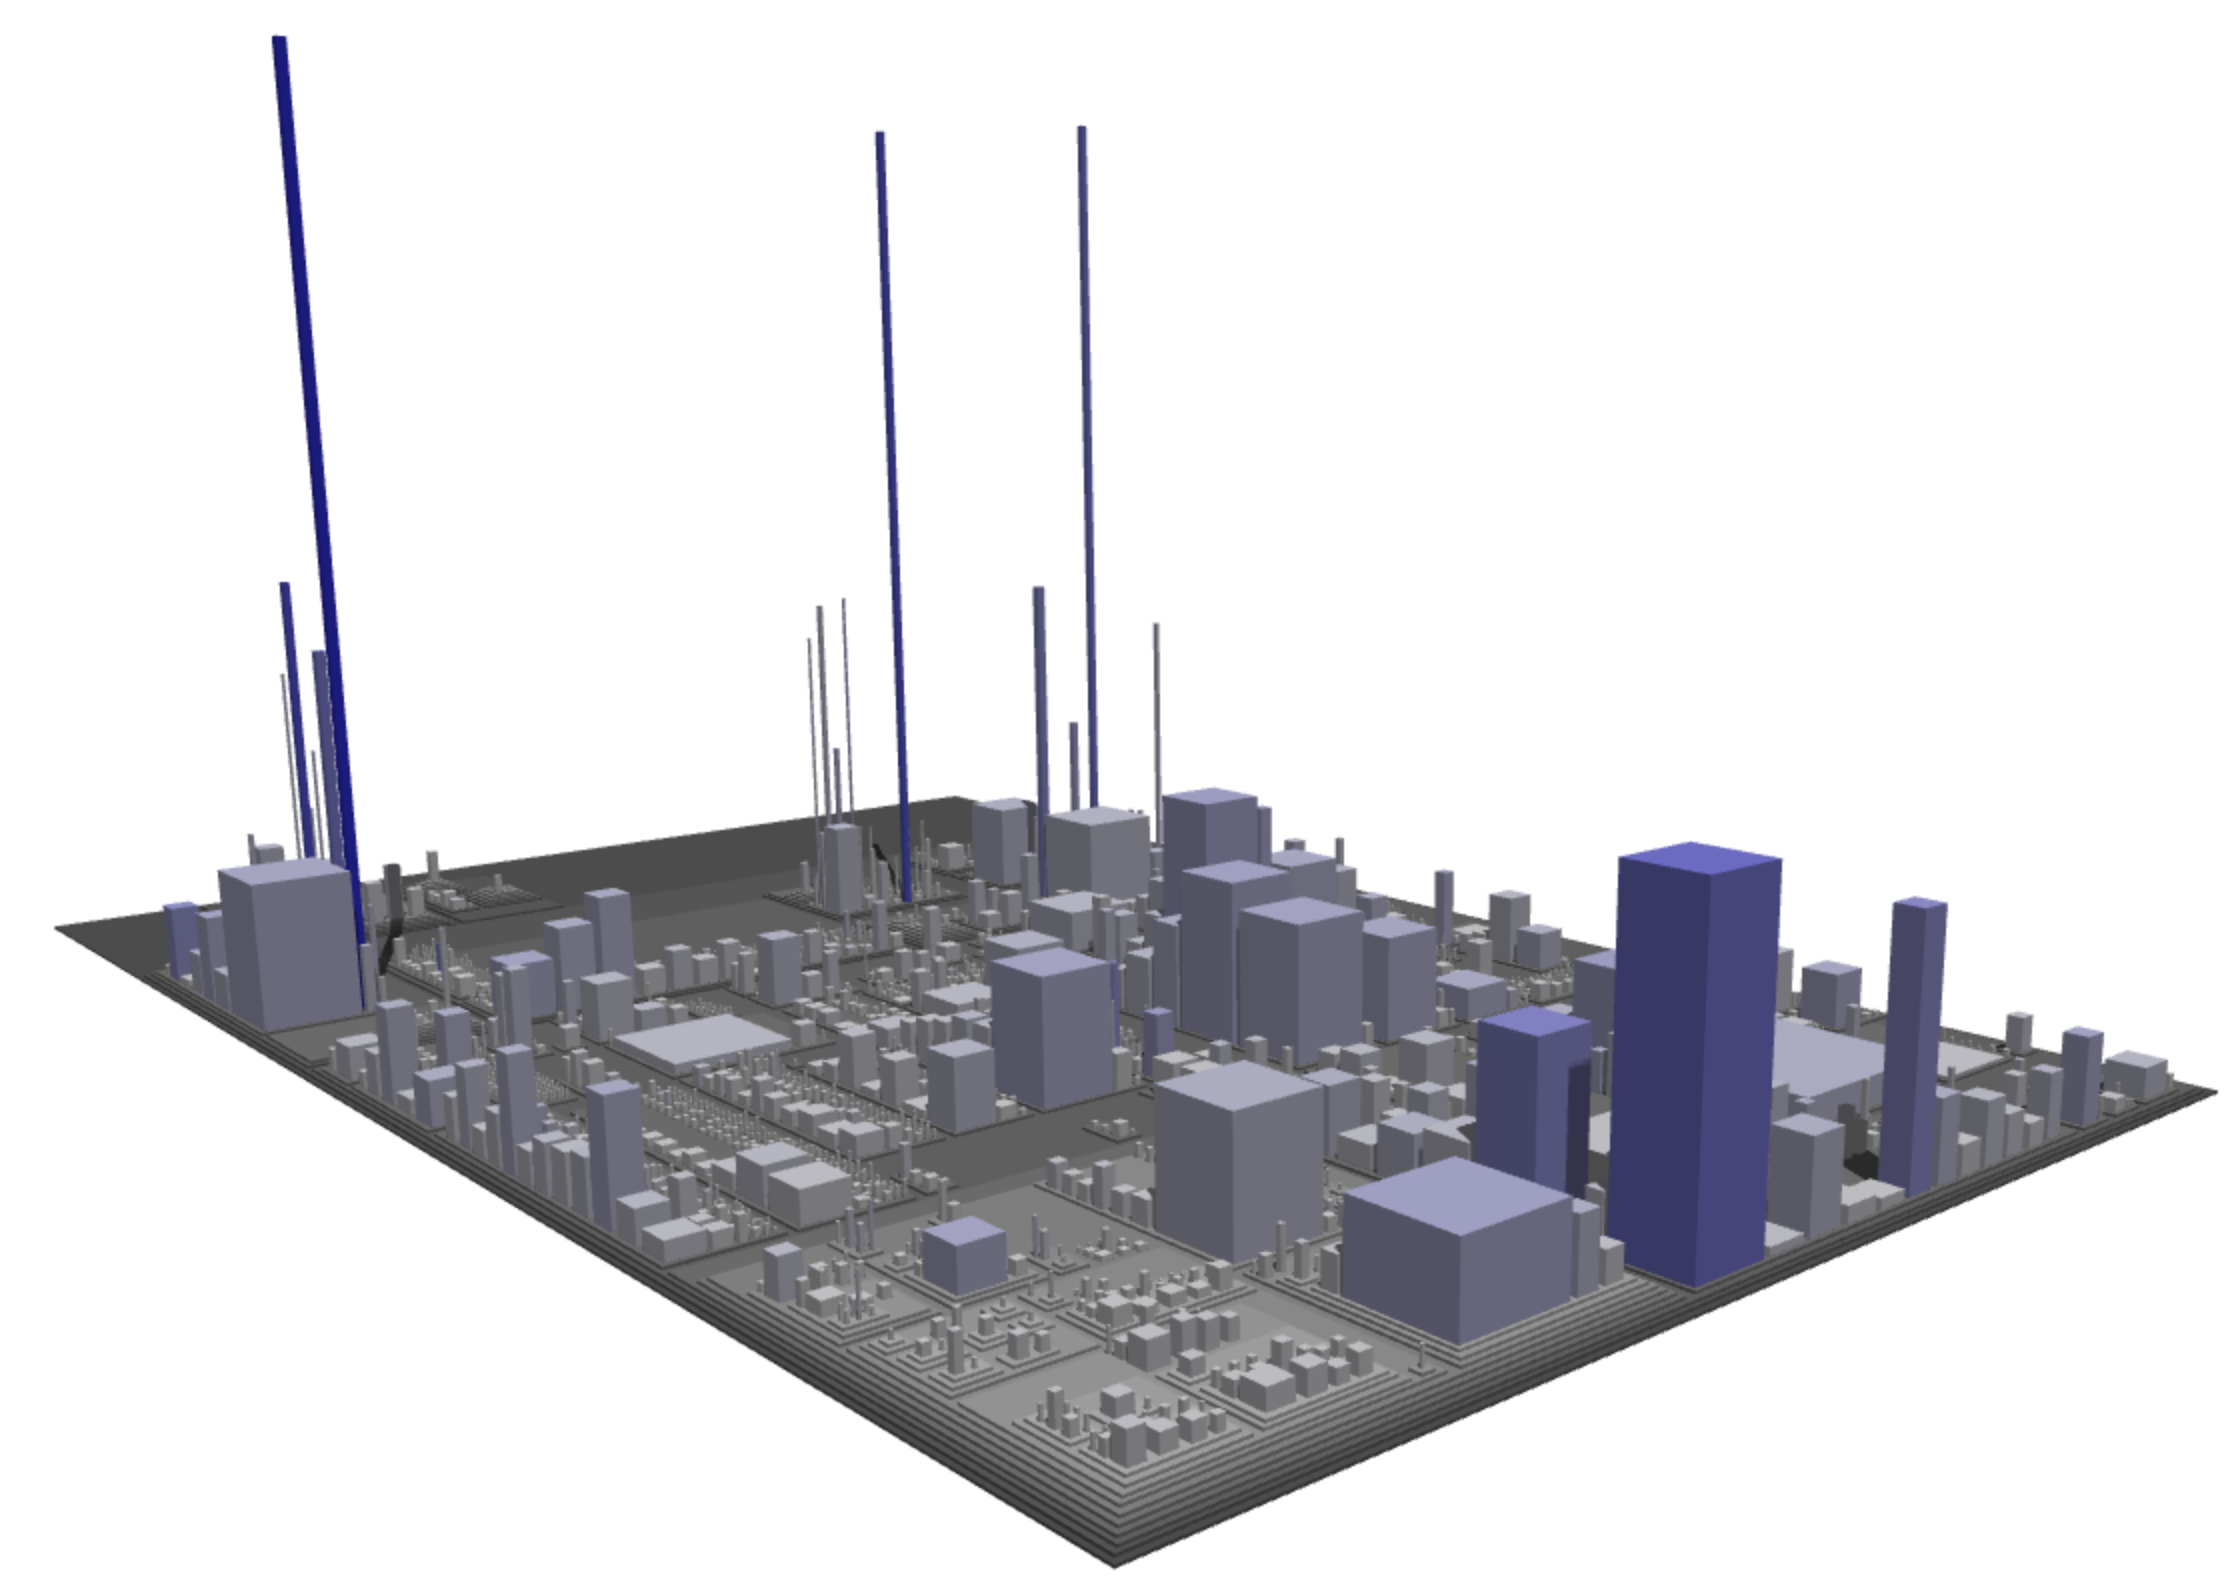
\includegraphics[width=.8\textwidth]{pictures/example.png}
\caption{A repository of ArgoUML visualized through WebCity}
\label{fig:example}
\end{figure}


%%%%%%%%%%%%%%%%%%%%%%%%%
\section{The model of the city} \label{The model of the city}
%%%%%%%%%%%%%%%%%%%%%%%%%
When we have to visualize something, it is very important to choose the right model that fits our data and that portrays the right information that the user is interested in. While in two dimensions there are some well established and common models -- pie charts, UML charts, scatterplots and so on -- when it comes to 3D visualizations there seems to be uncertainty on which models should be used and when.

When it comes to Software Visualization, and more specifically visualization of code written in Object Oriented languages, there is a model that has been used before \cite{Wett07b} \cite{Wett2008b} \cite{Wett2008a} with good results: the model of the city. This model has proved itself to be a solid choice because of some of its characteristics that make it suitable for our problem. Two of its strong points are the concept of familiarity -- which means that the user is not overwhelmed by the way that the information is portrayed, but instead he feels at ease in a familiar environment -- and the fact that that the code can be easily and meaningfully mapped to the model, because the way districts and buildings are positioned in a city is conceptually similar to how Java code is structured.

\subsection{Familiarity} \label{Familiarity}
One of the issues with many 3D visualizations is that they often do not appear intuitive or simple to understand, and they end up making things look more complicated than they actually are. A possible solution to this problem is using a model that the user is familiar and accustomed with. In our case, this model is the model of the city. Because everyone knows what cities are and how they are structured, this type of visualization ends up improving the system, making it more understandable and usable for the user.

\subsection{Connection between data and structure} \label{Connection between data and structure}
Since we are dealing with Software Visualization, this means that the data we want to portray comes from code, mostly written by people. In our case, this code is written in an Object Oriented programming language, Java.
Java code is structured in classes and packages, and the packages can recursively and contain other classes and packages.
This structure fits very well the model of the city: we can map the packages to districts of the city, and the classes to its buildings. This turns out to be a simple but efficient mapping between the data and the model.

The metrics of the classes can then be mapped to the dimensions and appearance of the classes:
the Number of Methods of a class is mapped to the height of the buildings, The Number of Attributes is mapped to their width and depth, and finally the number of Lines of Code is mapped to the color of the buildings.

In Figure \ref{fig:metrics} we can see an example of how these metrics are mapped. We can see buildings that look like skyscrapers because they have many methods and few fields, buildings that are almost flat that look like parking lots because they have many fields but few methods, and big buildings that have both many fields and methods, that could be called god classes \cite{Riel1996}.

\begin{figure} [H]
\centering
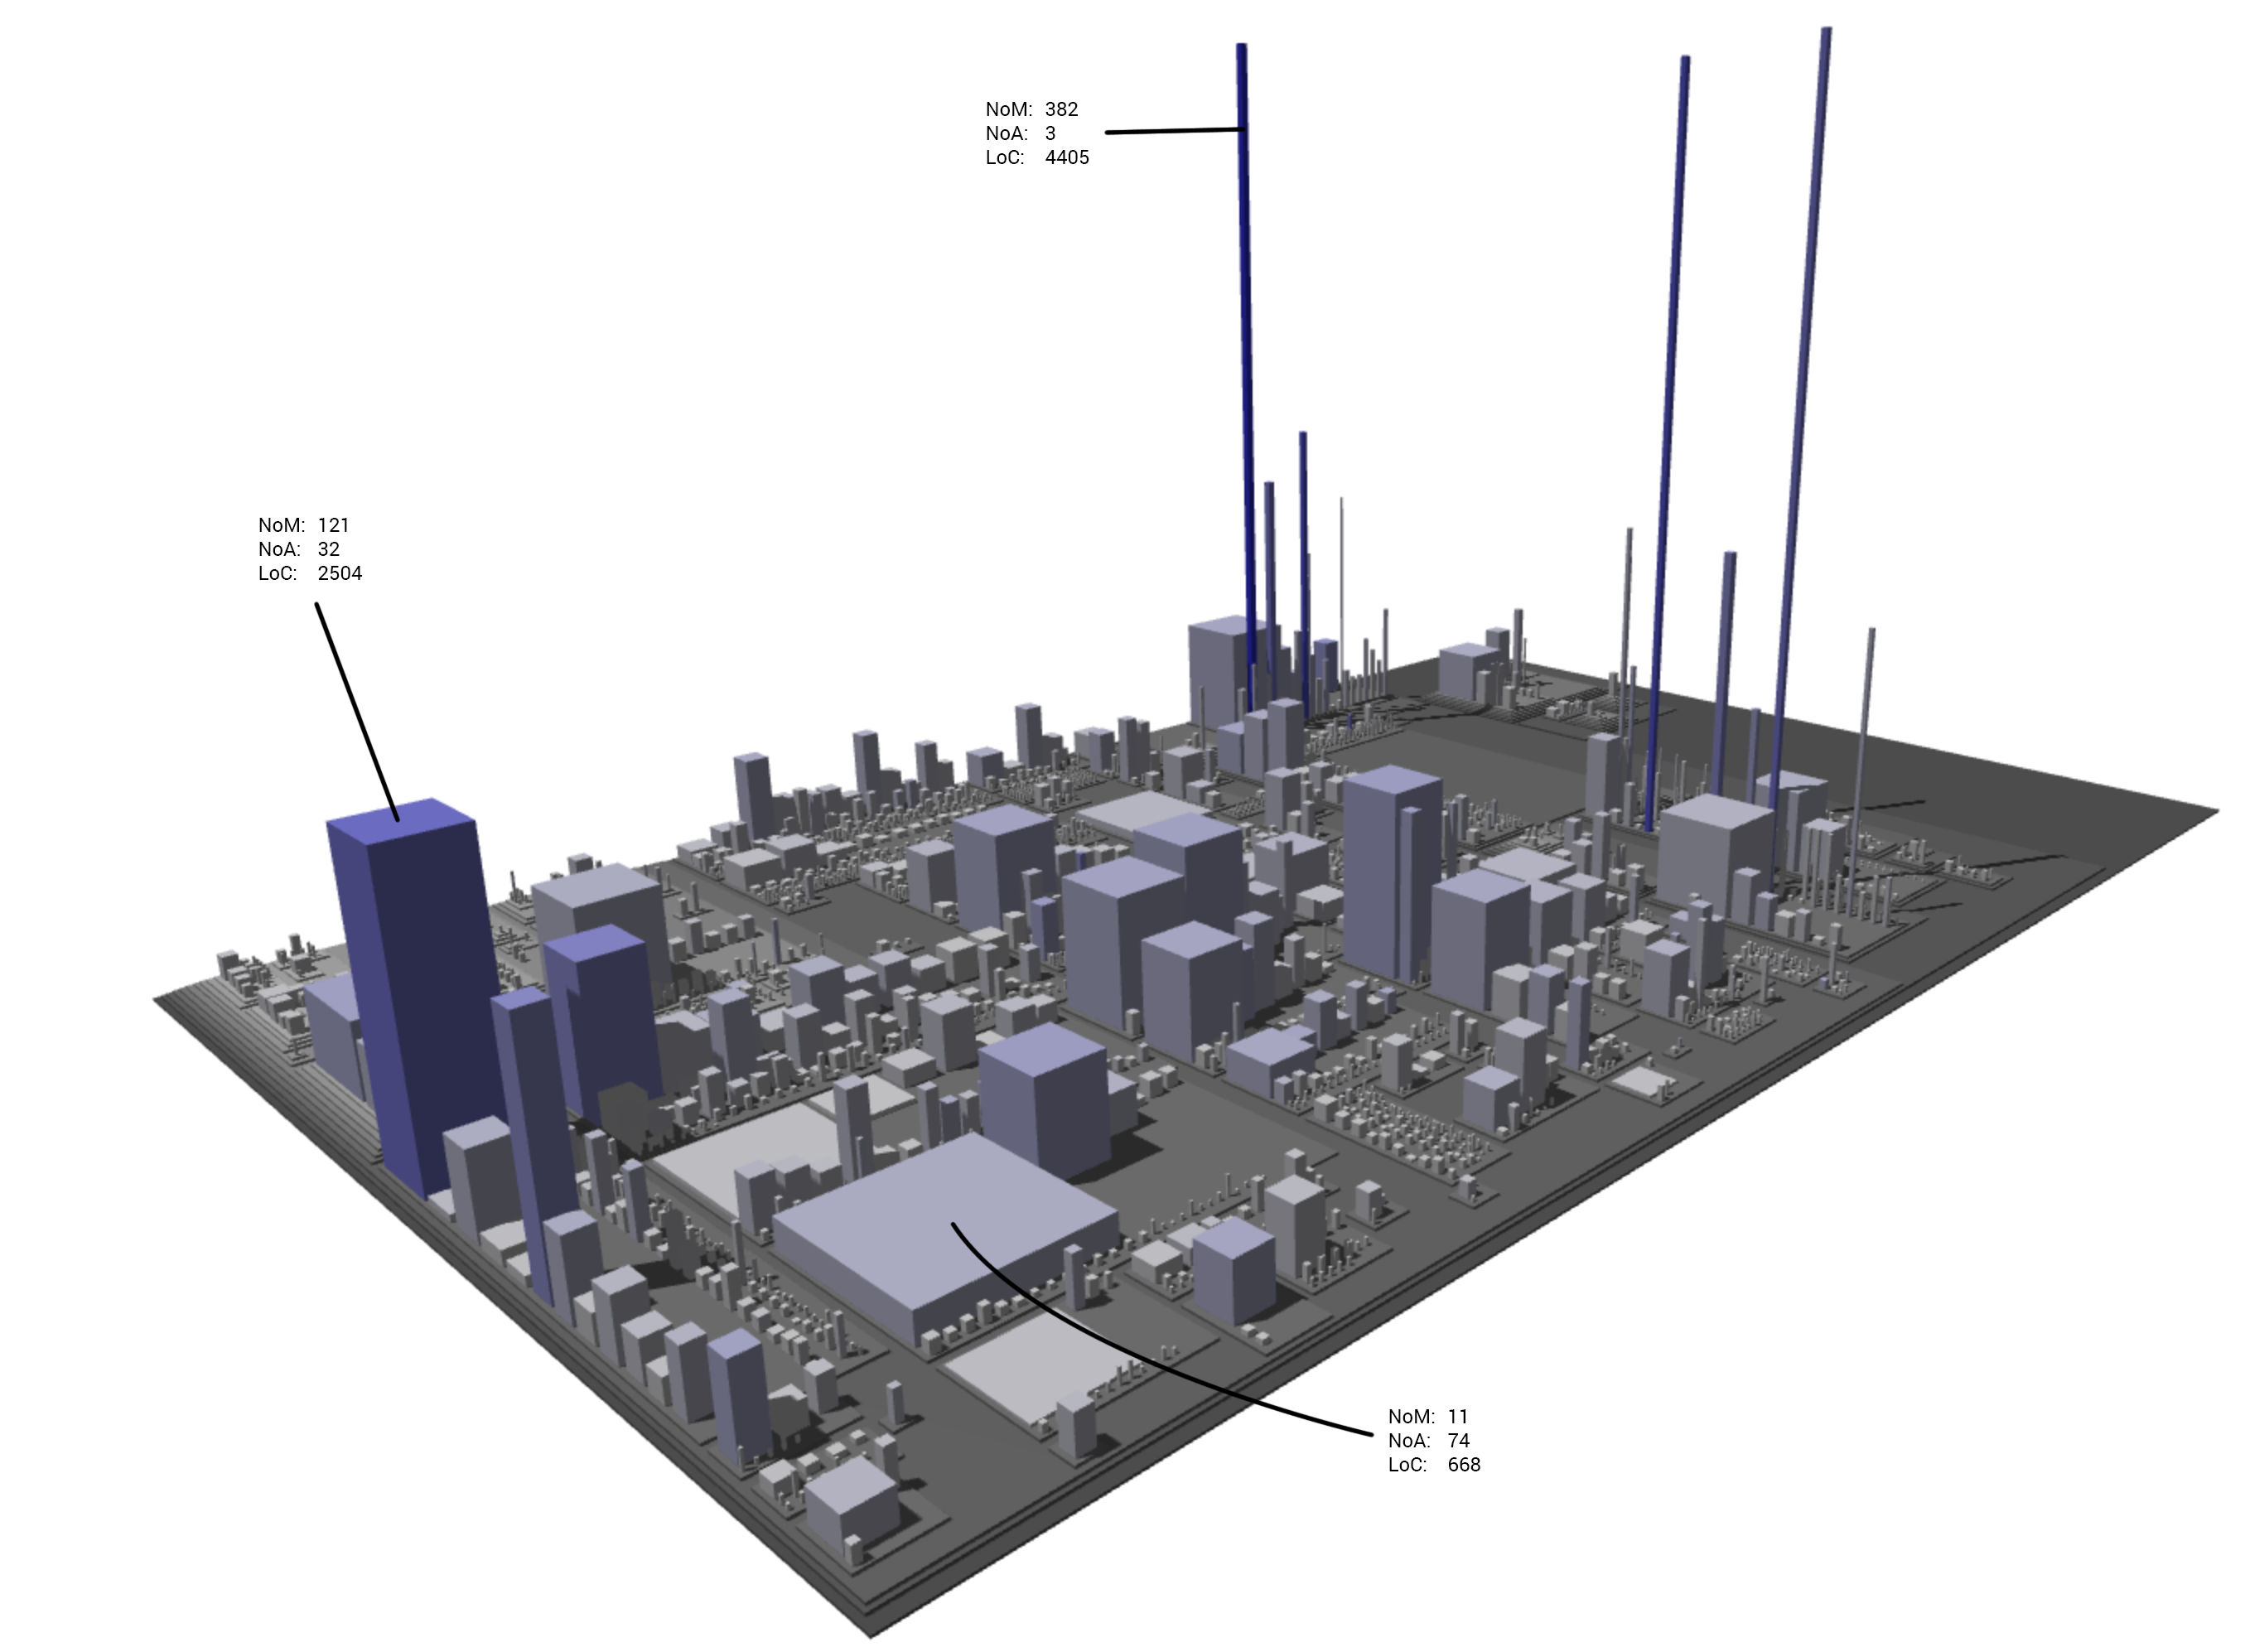
\includegraphics[width=1\textwidth]{pictures/metrics.png}
\caption{A visual explanation of how the metrics are mapped}
\label{fig:metrics}
\end{figure}



%%%%%%%%%%%%%%%%%%%%%%%%%
\section{The application} \label{WebCity}
%%%%%%%%%%%%%%%%%%%%%%%%%

The application aims to have a simple yet usable design. Most of the browser's window is occupied by the visualization (see Figure \ref{fig:app}). The information about the visualization is displayed on the right side: the name of the currently focused element, a list of metrics depending on the type of element we are hovering (class or package),
and at the bottom the number of total classes of the whole visualization, to give us an idea of the order of magnitude of the version of the system we are currently seeing.

The header bar contains the search input field, which can be used to look for specific objects, the camera icon that pops up the options to generate a video of the visualization, the cog icon that pops up a list of options to change how the paddings, classes and packages are sized, and on the far right a drop-down menu that contains the list of versions (commits or tags) that the user can select to choose which version he wants to be displayed.
On the bottom right there's a question mark icon, that pops up a help window that explains how to navigate and interact with the 3D environment.

\begin{figure} [H]
\centering
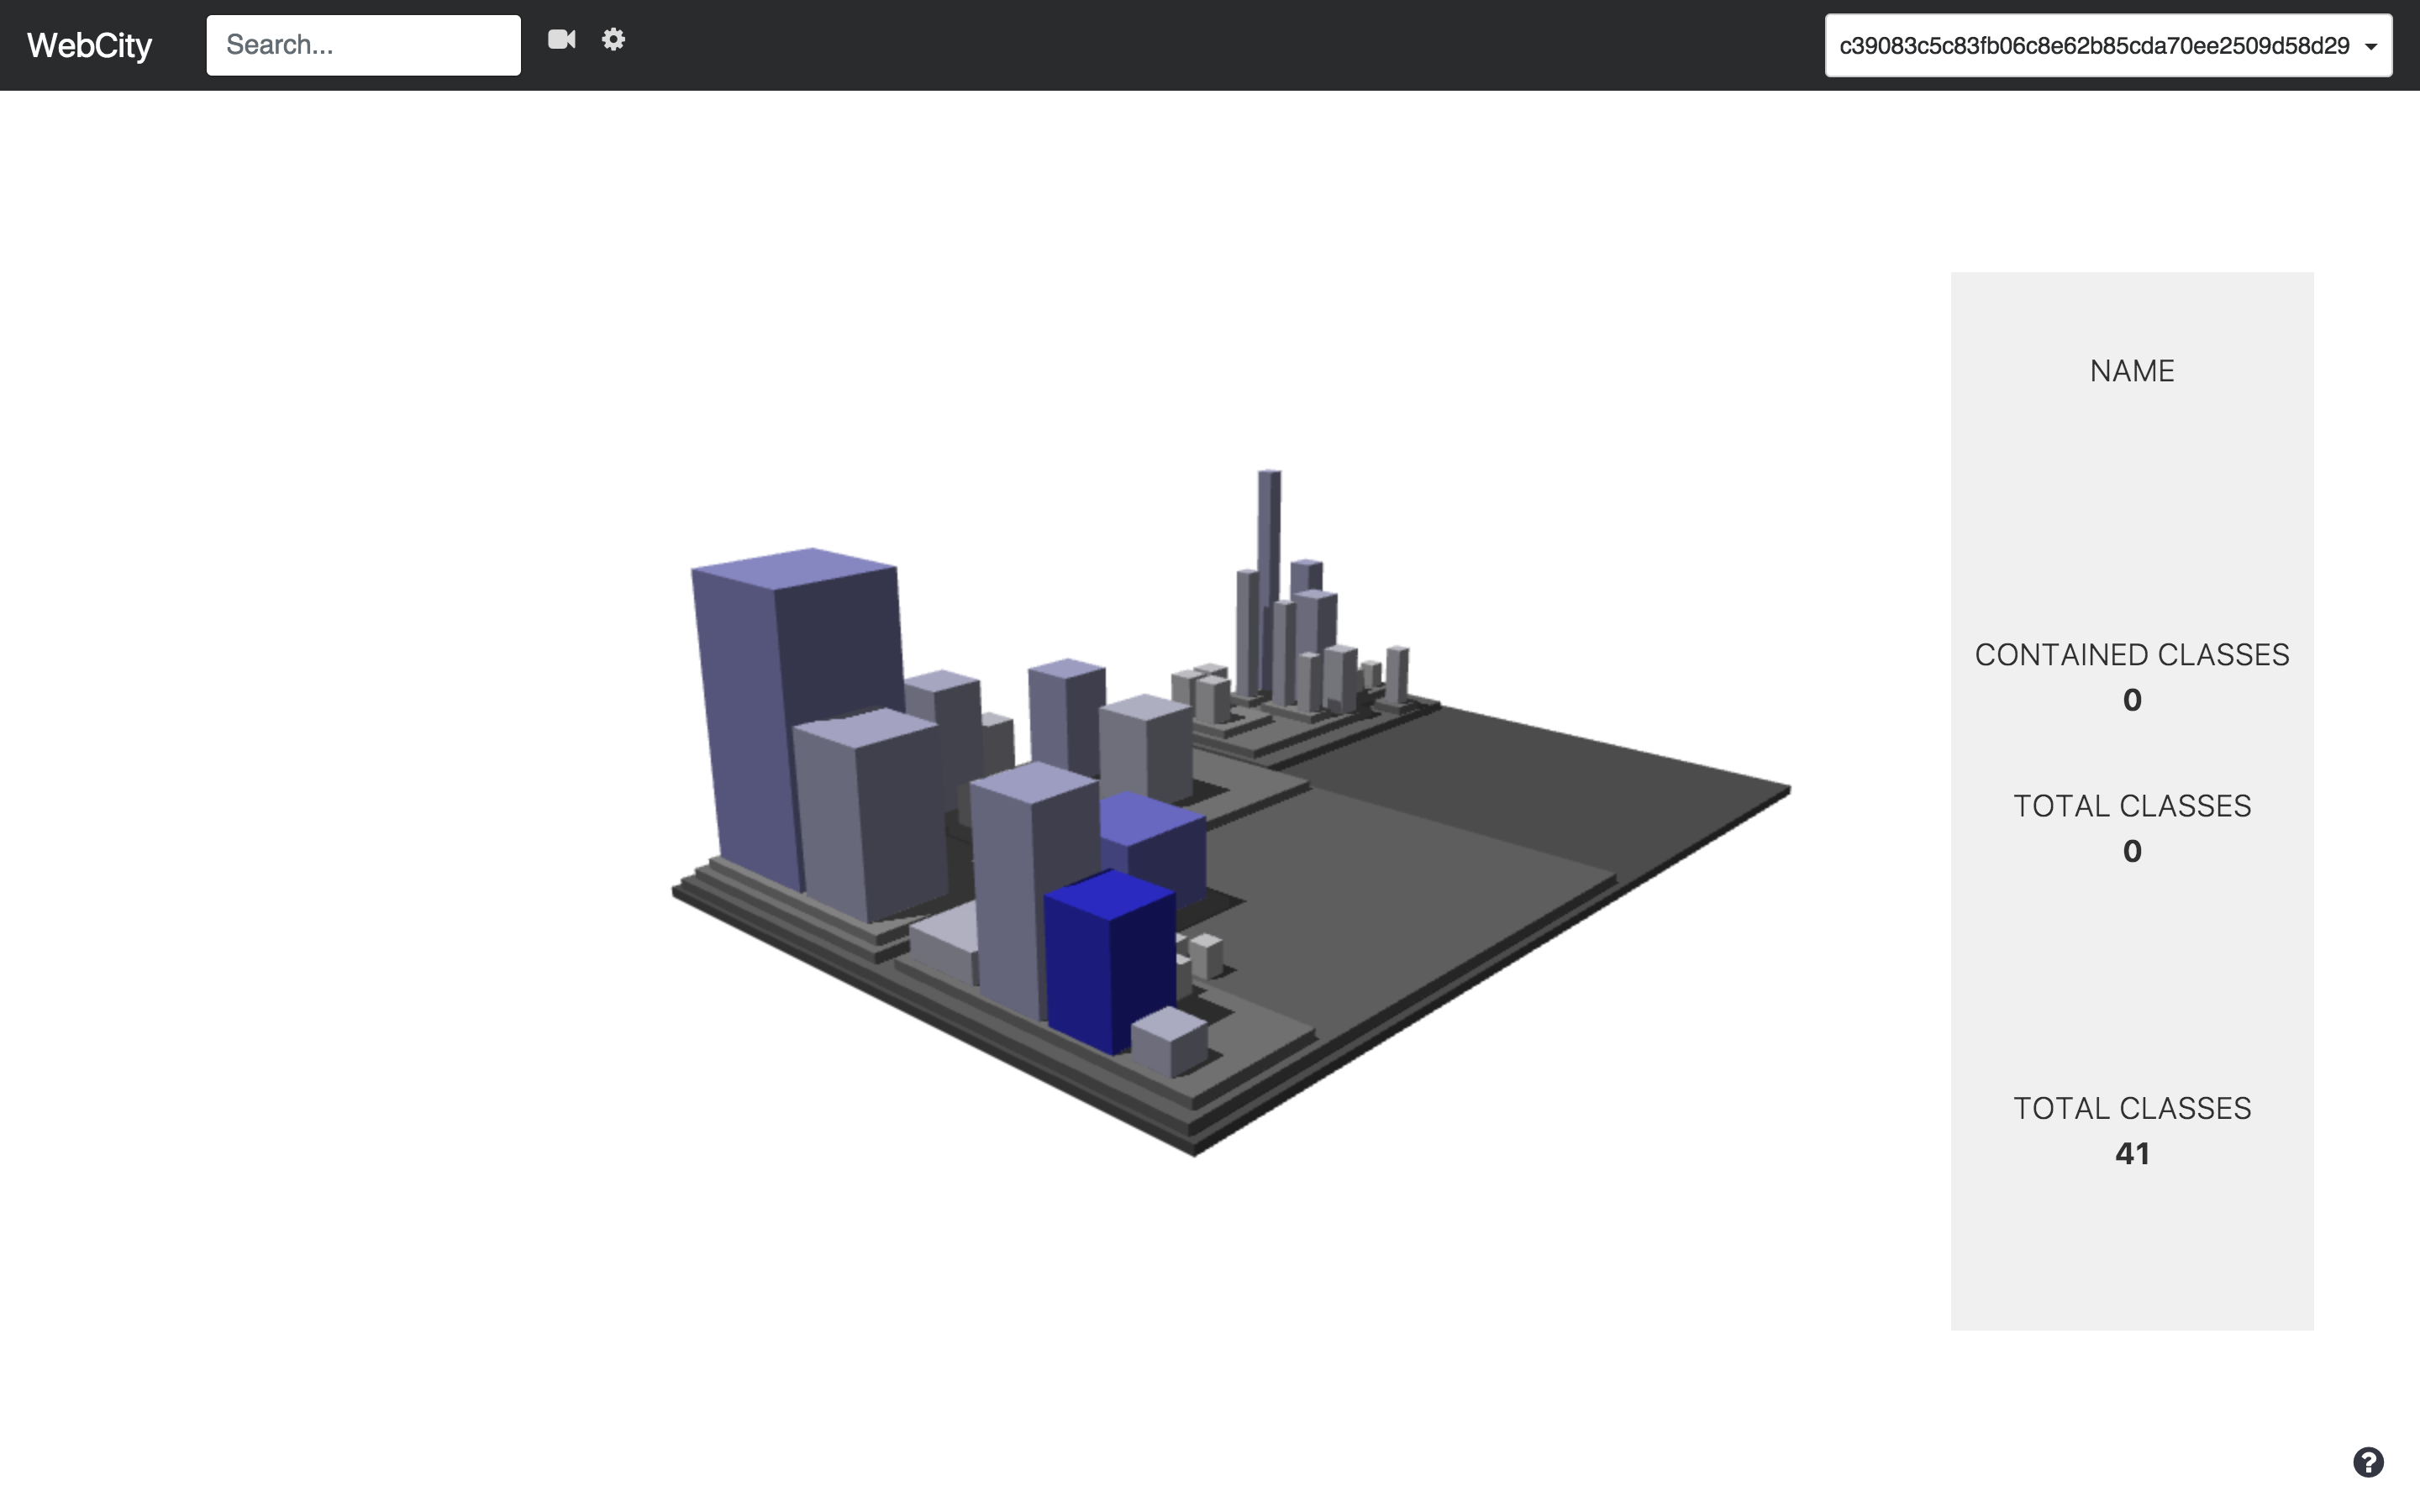
\includegraphics[width=1\textwidth]{pictures/app.png}
\caption{What the application looks like}
\label{fig:app}
\end{figure}

\subsection{Interface} \label{Interface}

When we open the main page of the application, the only thing on screen is an input field where the user can write the address of a public GitHub repository. This minimalistic design is aimed at simplifying the experience for the users and improving the usability. Once the user inputs a valid repository and clicks the submit button, the application downloads the required data from GitHub to the server. Then the user has the choice between a visualization that is based on commits or tags; most of the time the number of tags is many times smaller than the number of commits, which makes the parsing of the versions of the repository faster and reduces the waiting time for the user. Once the user has chosen and accepted the visualization type, the application starts parsing the code of the repository and loads the 3D visualization on screen.

% \begin{figure}[H]
% \centering
%   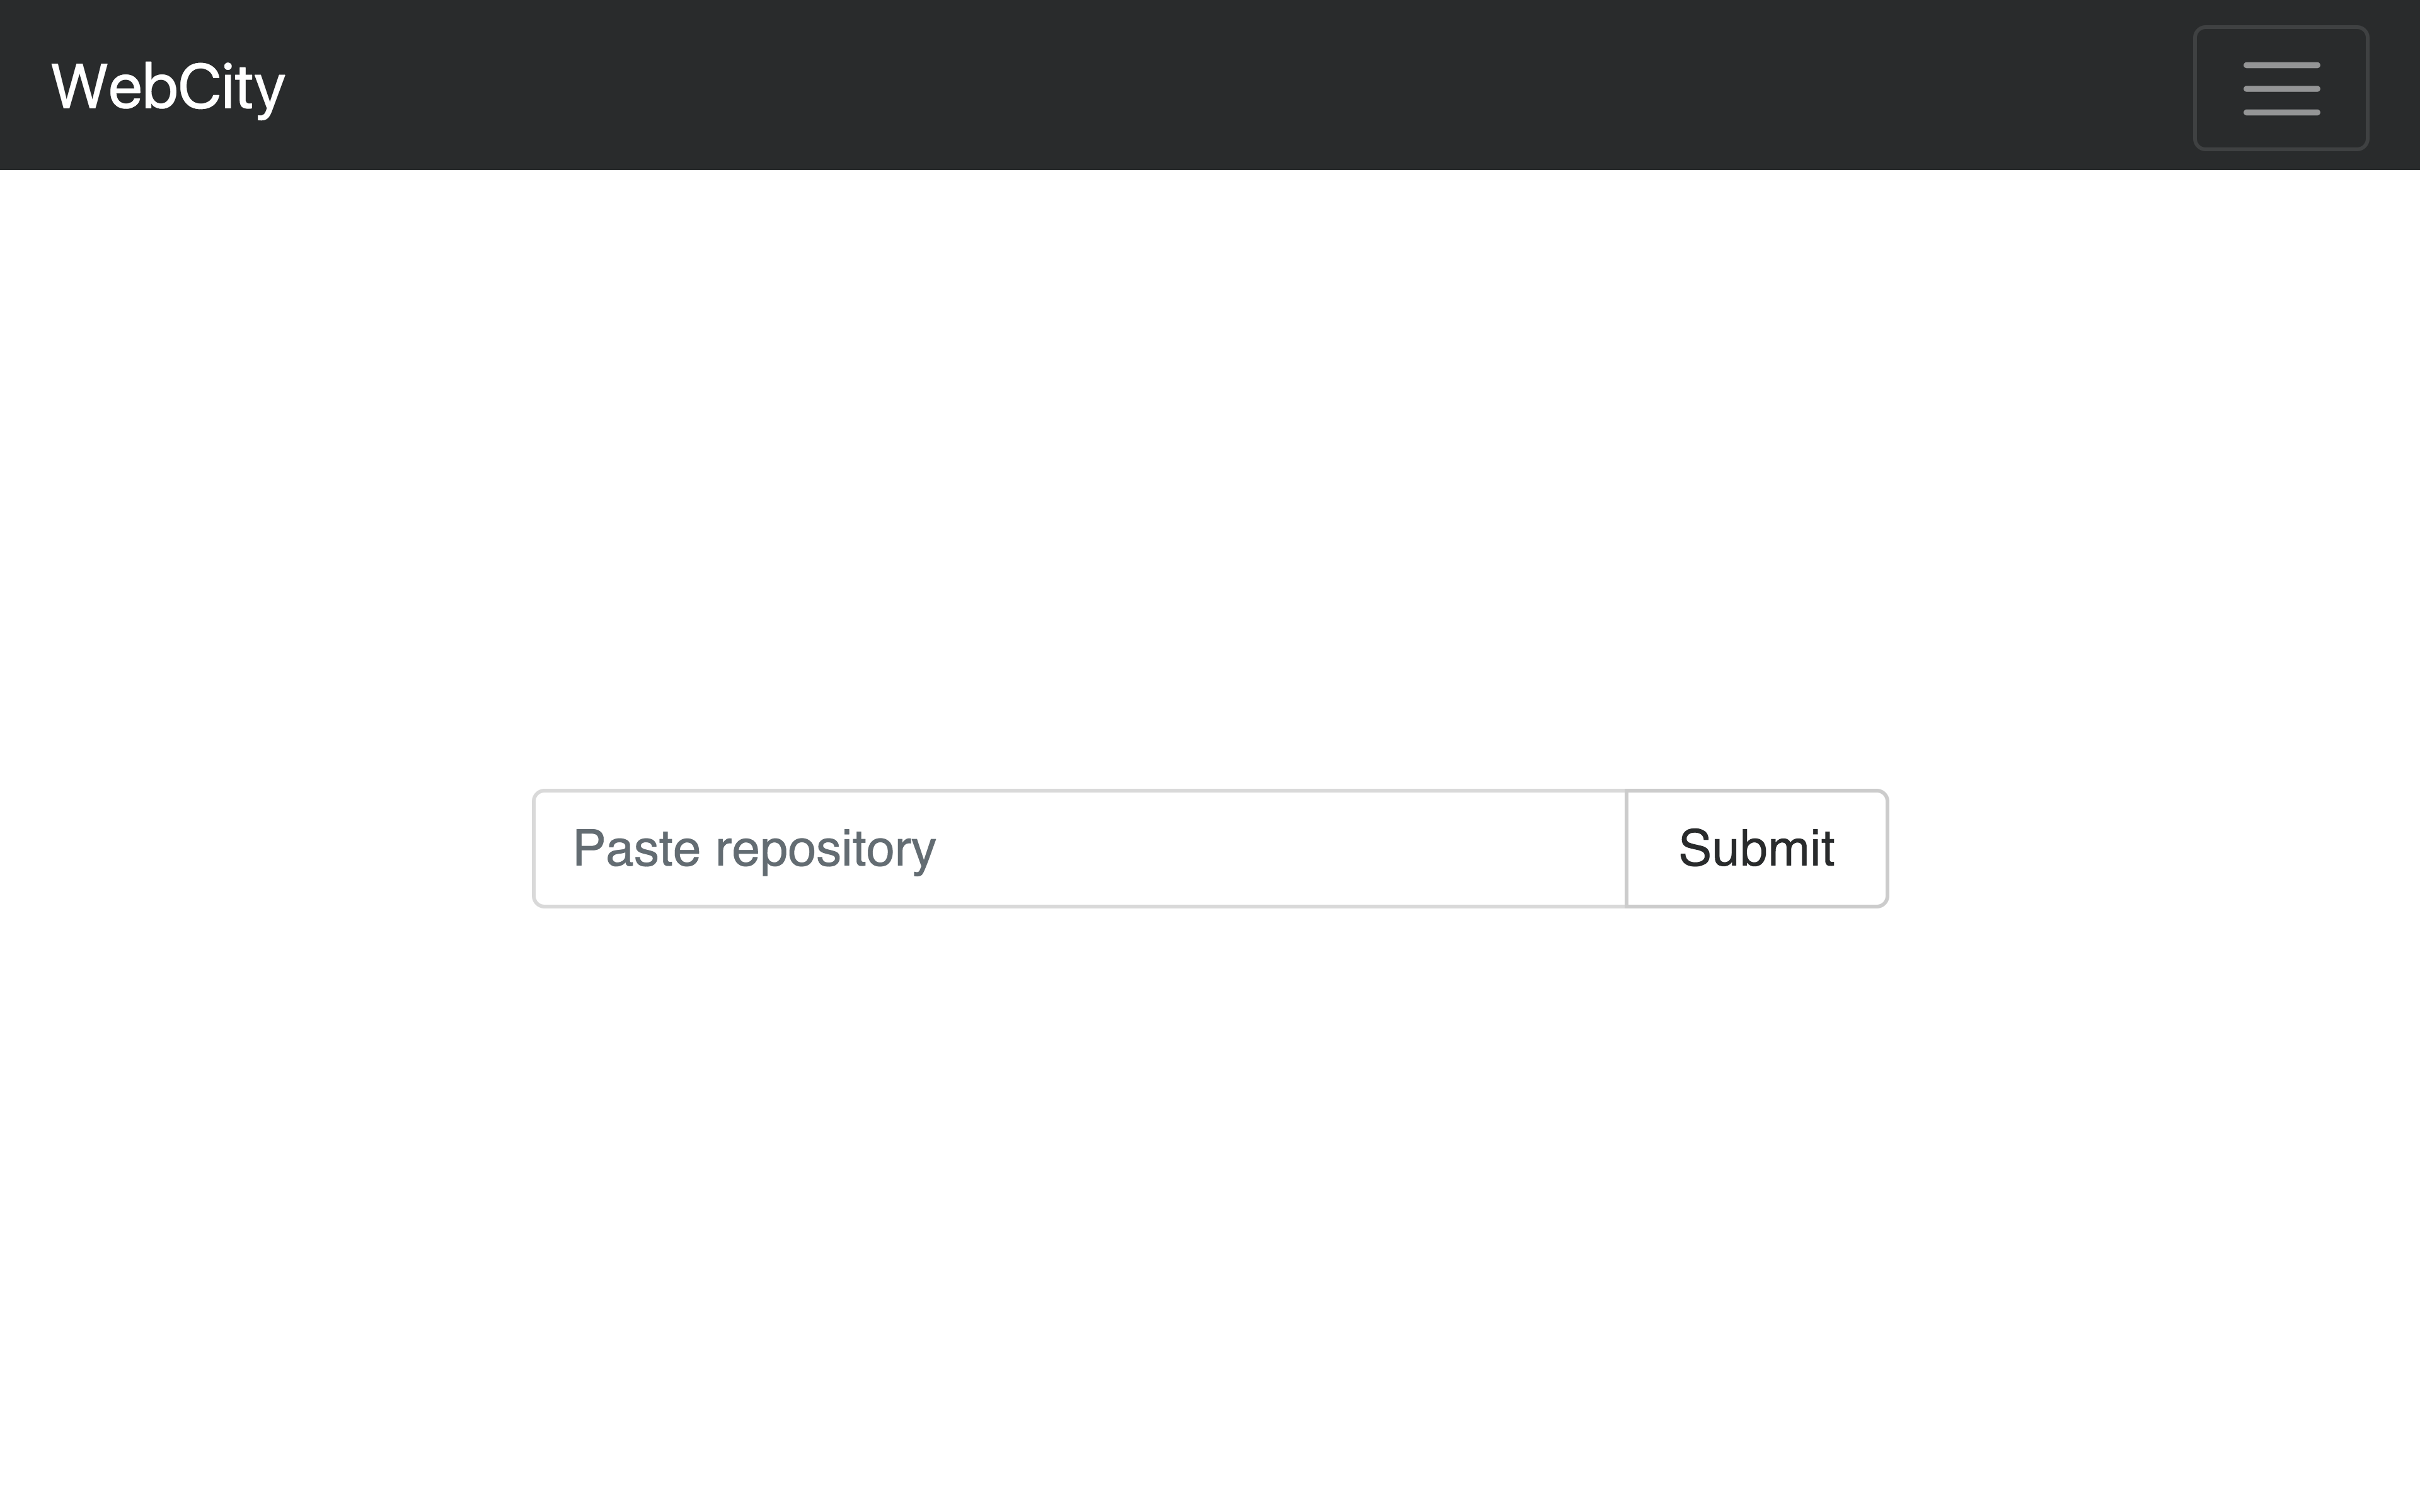
\includegraphics[width=.6\textwidth]{pictures/interface.png}
%   \caption{The minimalistic main page}
%   \label{fig:interface}
% \end{figure}
%
% \begin{figure}[H]
%     \centering
%   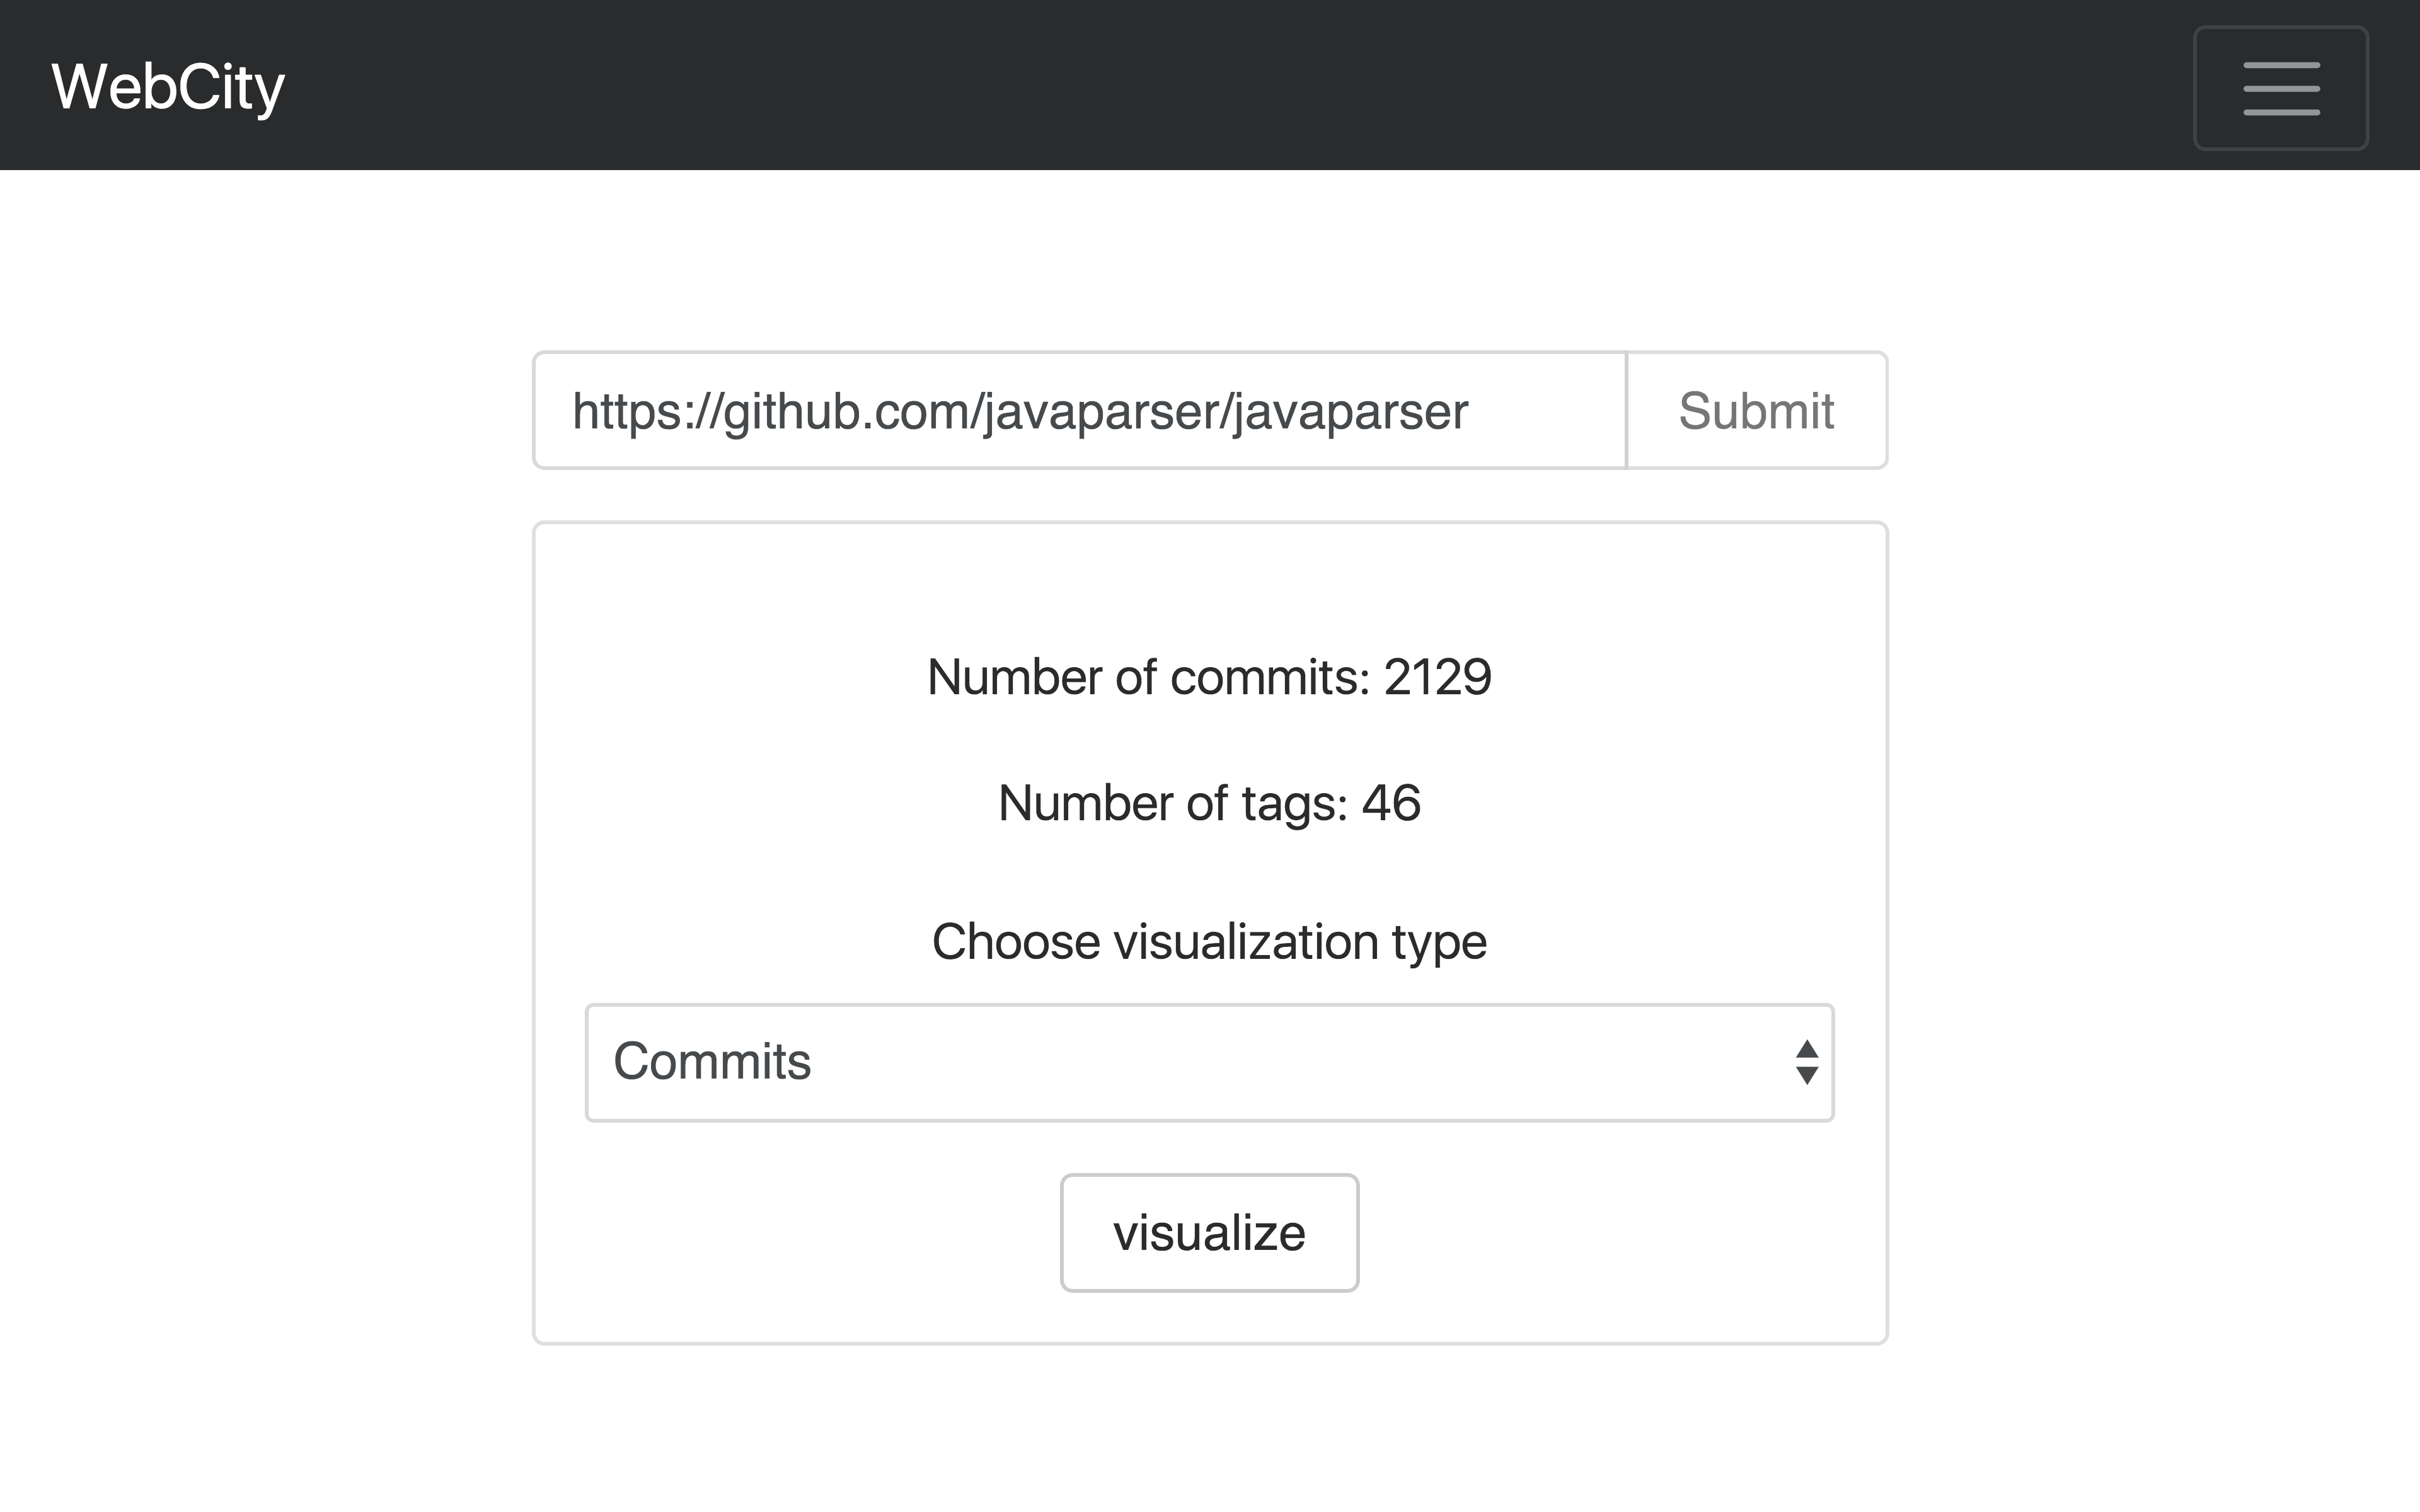
\includegraphics[width=.6\textwidth]{pictures/interface2.png}
%   \caption{The view that allows to choose visualization}
%   \label{fig:interface2}
% \end{figure}
%
% \begin{figure} [H]
% \centering
% 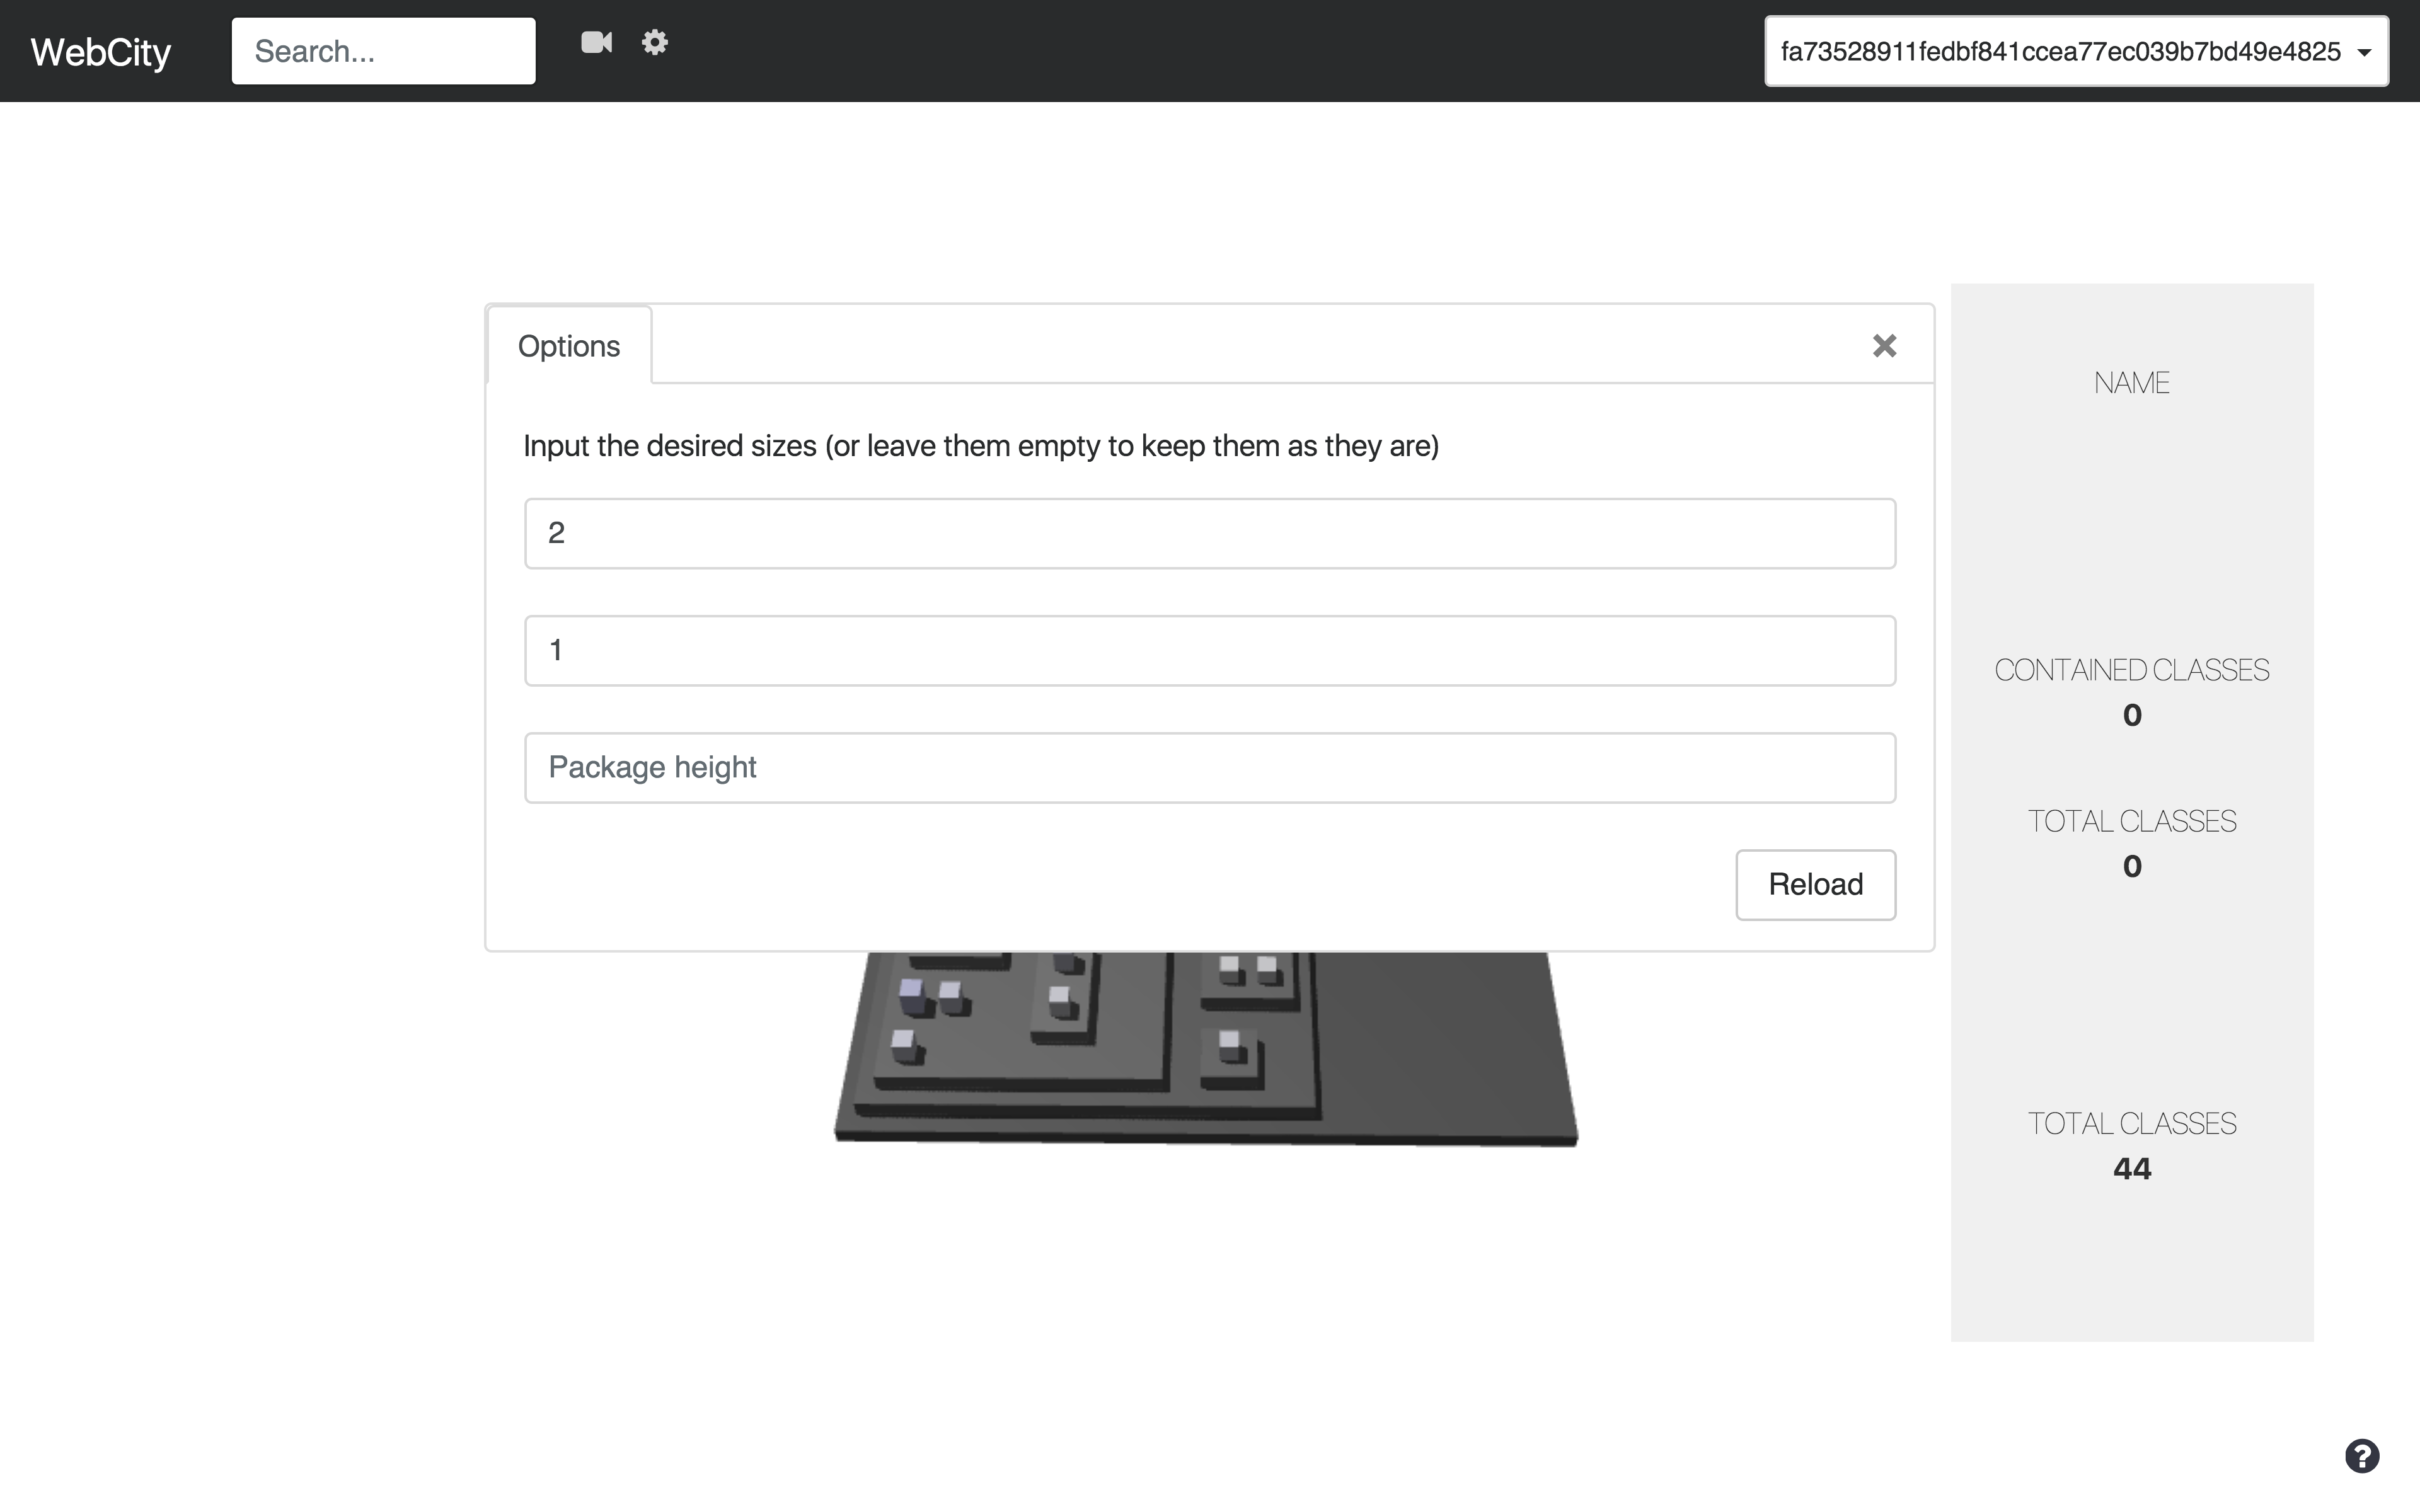
\includegraphics[width=1\textwidth]{pictures/sizing_card.png}
% \caption{The options to set the sizing of the visualization}
% \label{fig:sizing}
% \end{figure}

\begin{figure}[H]
  \centering
  \begin{minipage}[b]{0.49\textwidth}
      \centering
      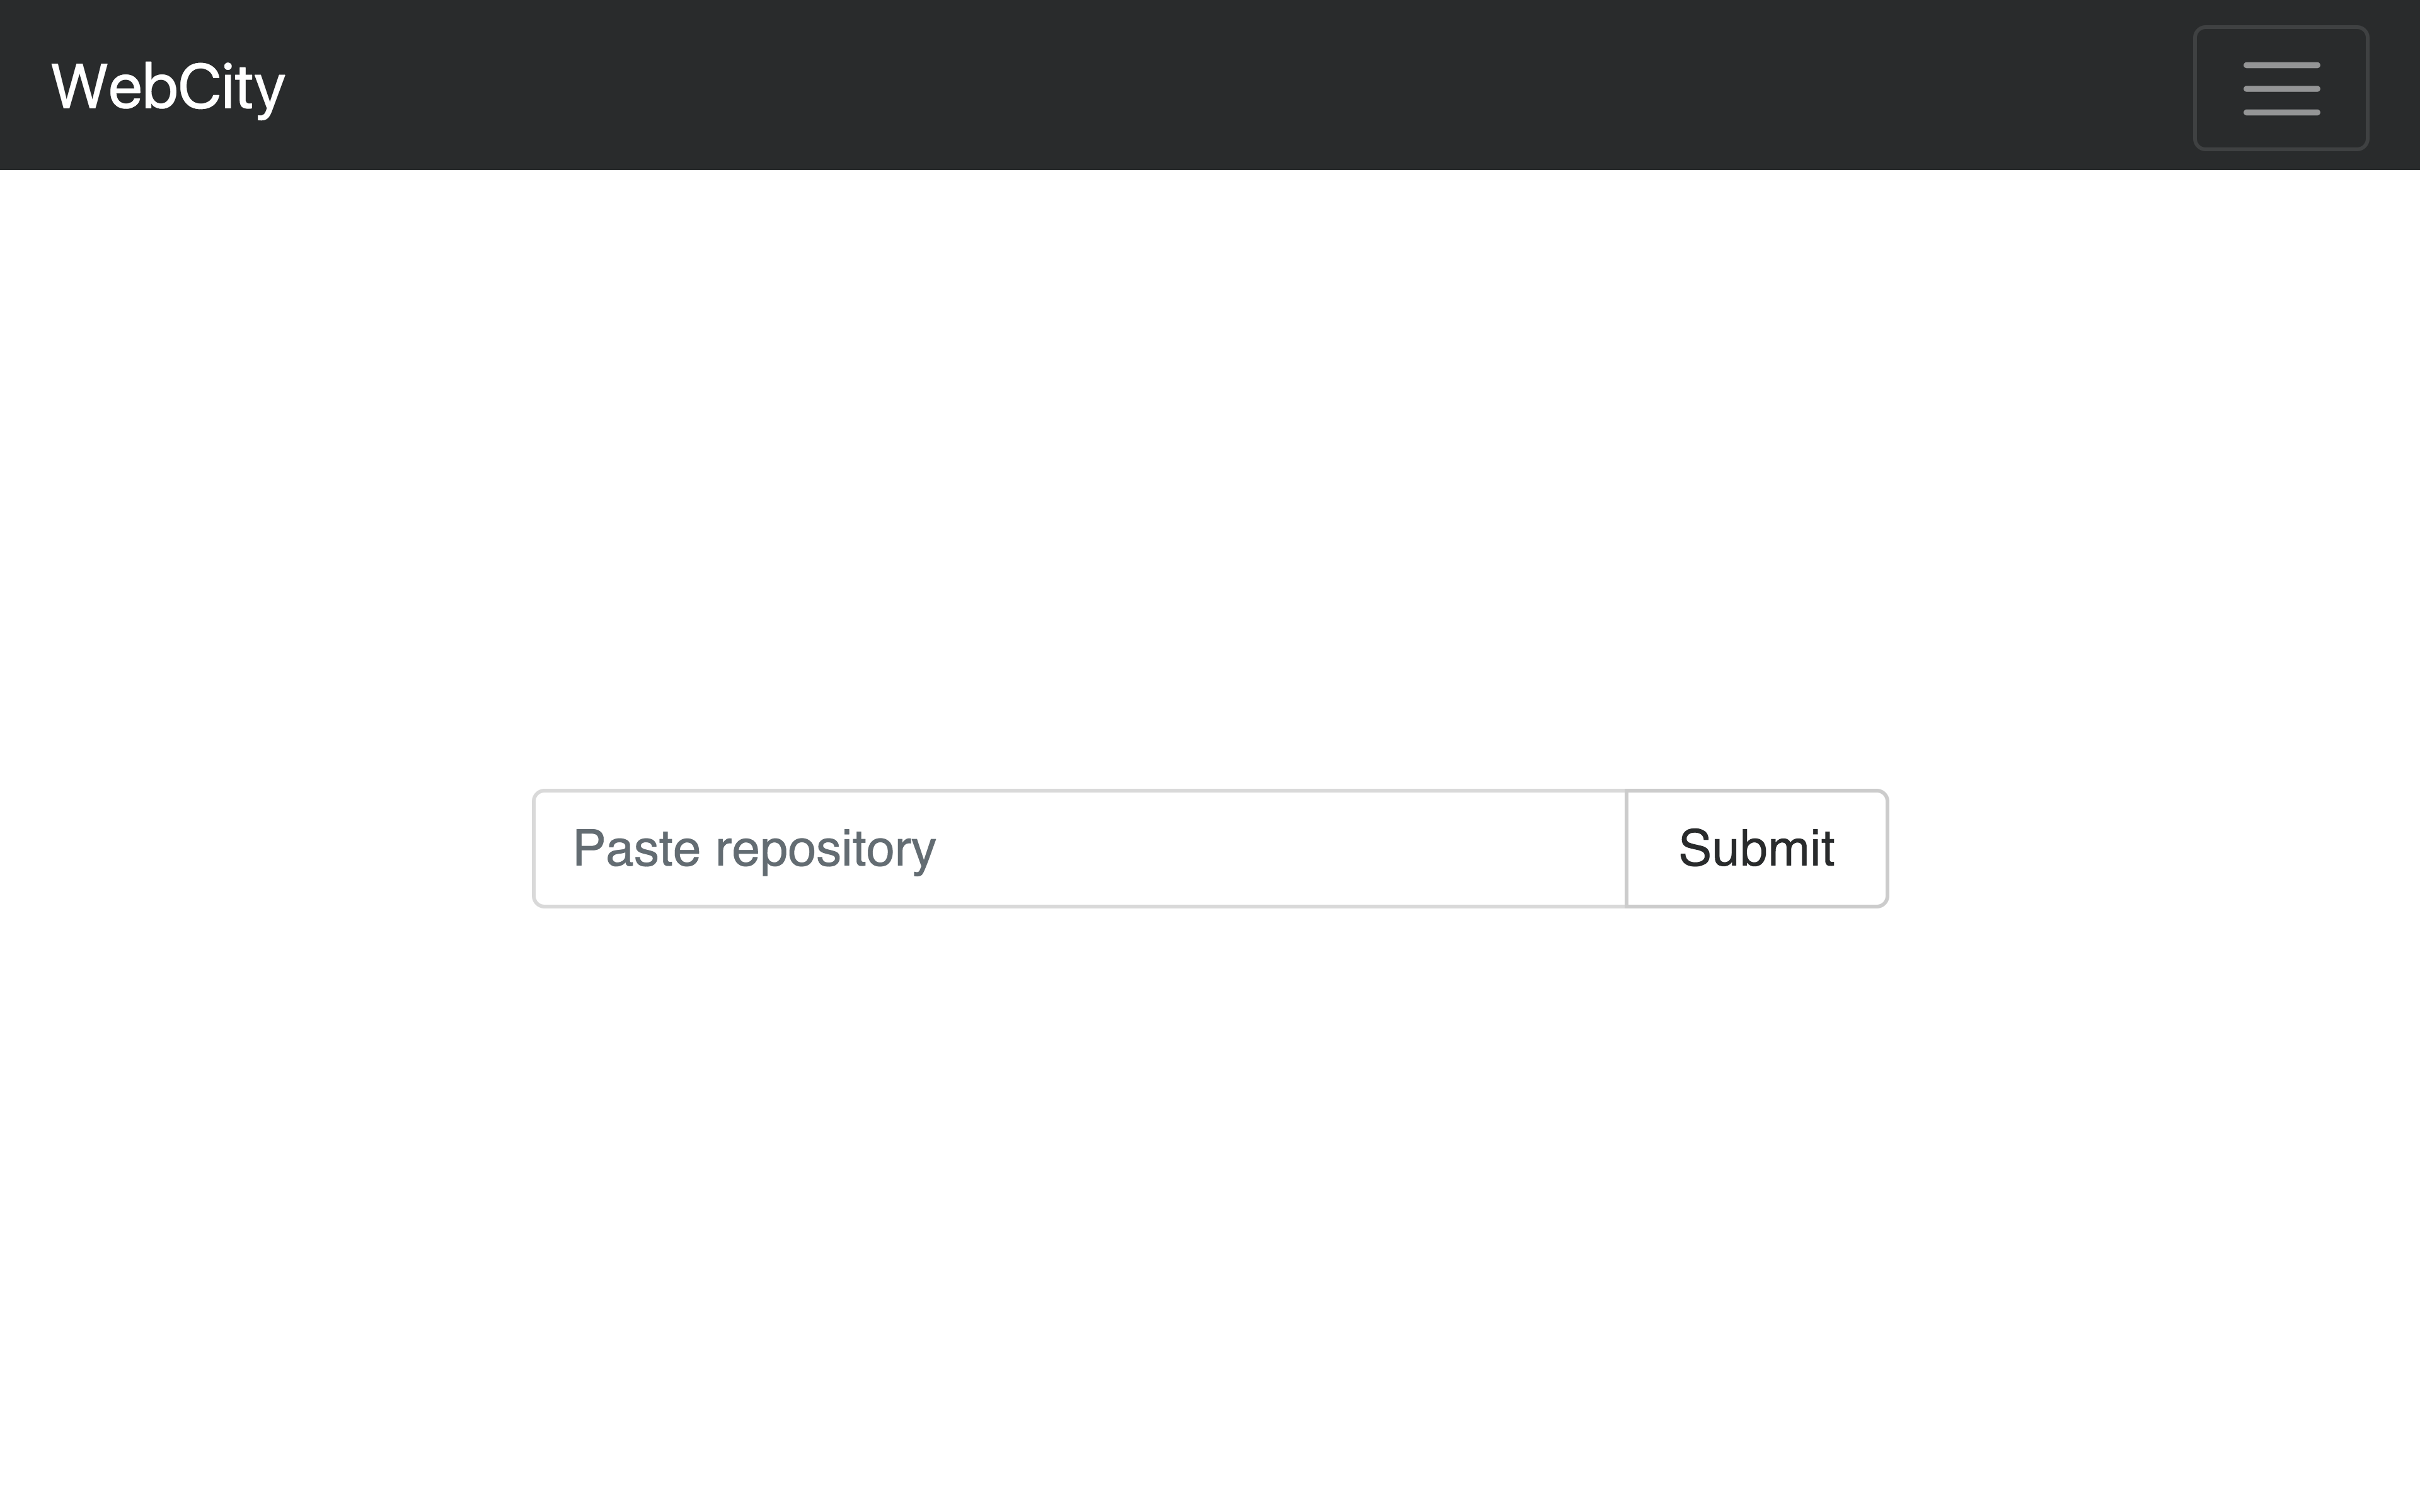
\includegraphics[width=1\textwidth]{pictures/interface.png}
      \caption{The minimalistic main page}
      \label{fig:interface}
  \end{minipage}
  \hfill
  \begin{minipage}[b]{0.49\textwidth}
      \centering
      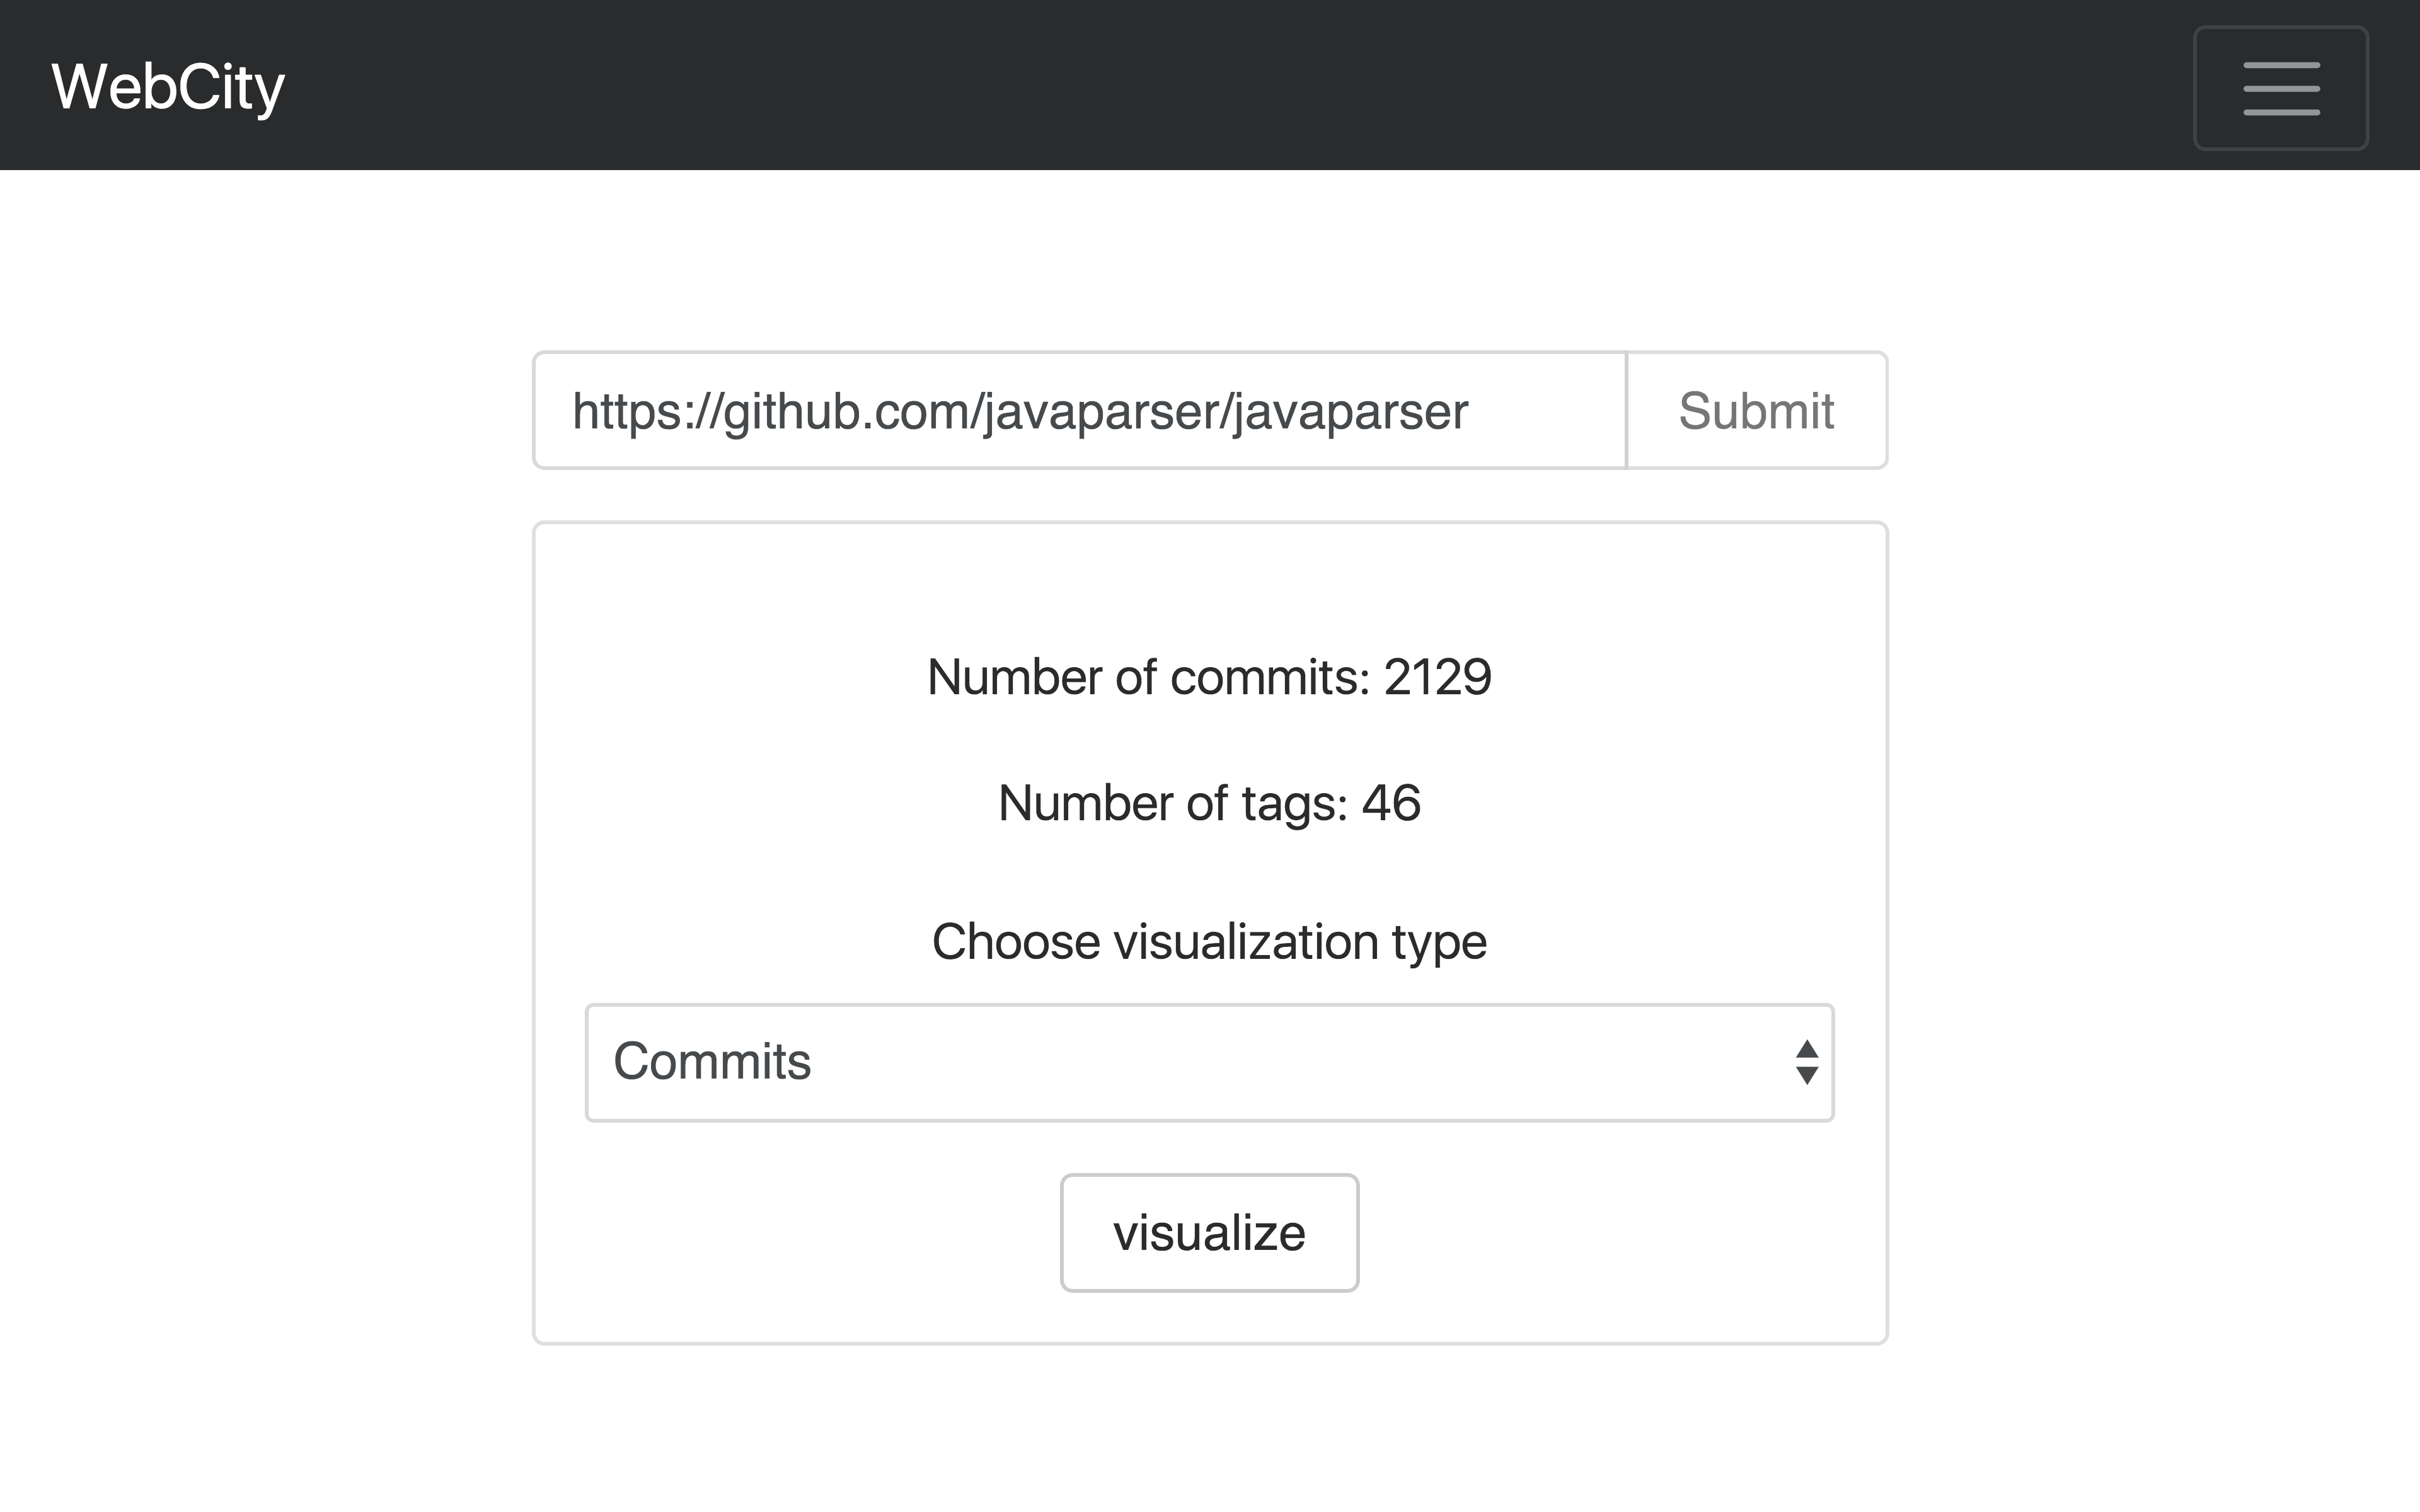
\includegraphics[width=1\textwidth]{pictures/interface2.png}
      \caption{The view that allows to choose visualization}
      \label{fig:interface2}
  \end{minipage}
\end{figure}

\subsection{Interaction} \label{Interaction}
Because of how big the cities can become, we implemented a set of features to make it easier for the users to find what they are looking for, while also not getting lost by doing so. These features include hovering, searching, tagging, and visualization of source code.

\subsubsection{Hover} \label{Hover}
Hovering on the elements of the visualization will show on screen some important metrics and other information about these elements.
When we hover on a class, the screen will show the name of the class itself plus the name of the file it is contained in. It will also show the Number of Methods,
 the Number of Attributes and the Lines of Code of that specific class.

 If instead the user hovers on a package, its name will be displayed, in addition to the number of contained classes -- the classes that are directly contained in this package, at one depth of traversal --
  and the number of total classes, that also accounts for the classes contained in the children packages of the current package we are hovering.

\subsubsection{Search} \label{Search}
Finding the exact class or package that we are looking for can be difficult to do, even harder if it is a very small building in the middle of the city.
The search function we implemented allows to filter through all the elements of the visualization. While the user types,
the list of matching elements updates to only show the ones that match the input field. The user can then select the desired item of the list to have the camera point to it,
and have its color changed to be able to tell it apart from the other elements.
Figure \ref{fig:tag} shows the user looking for ``JavaPac'' in the search bar, and getting a list of results that match the input text; when then the user selected ``app/models/JavaPackage.java:JavaPackage'' the building got highlighted and the camera focused it.

\begin{figure} [H]
\centering
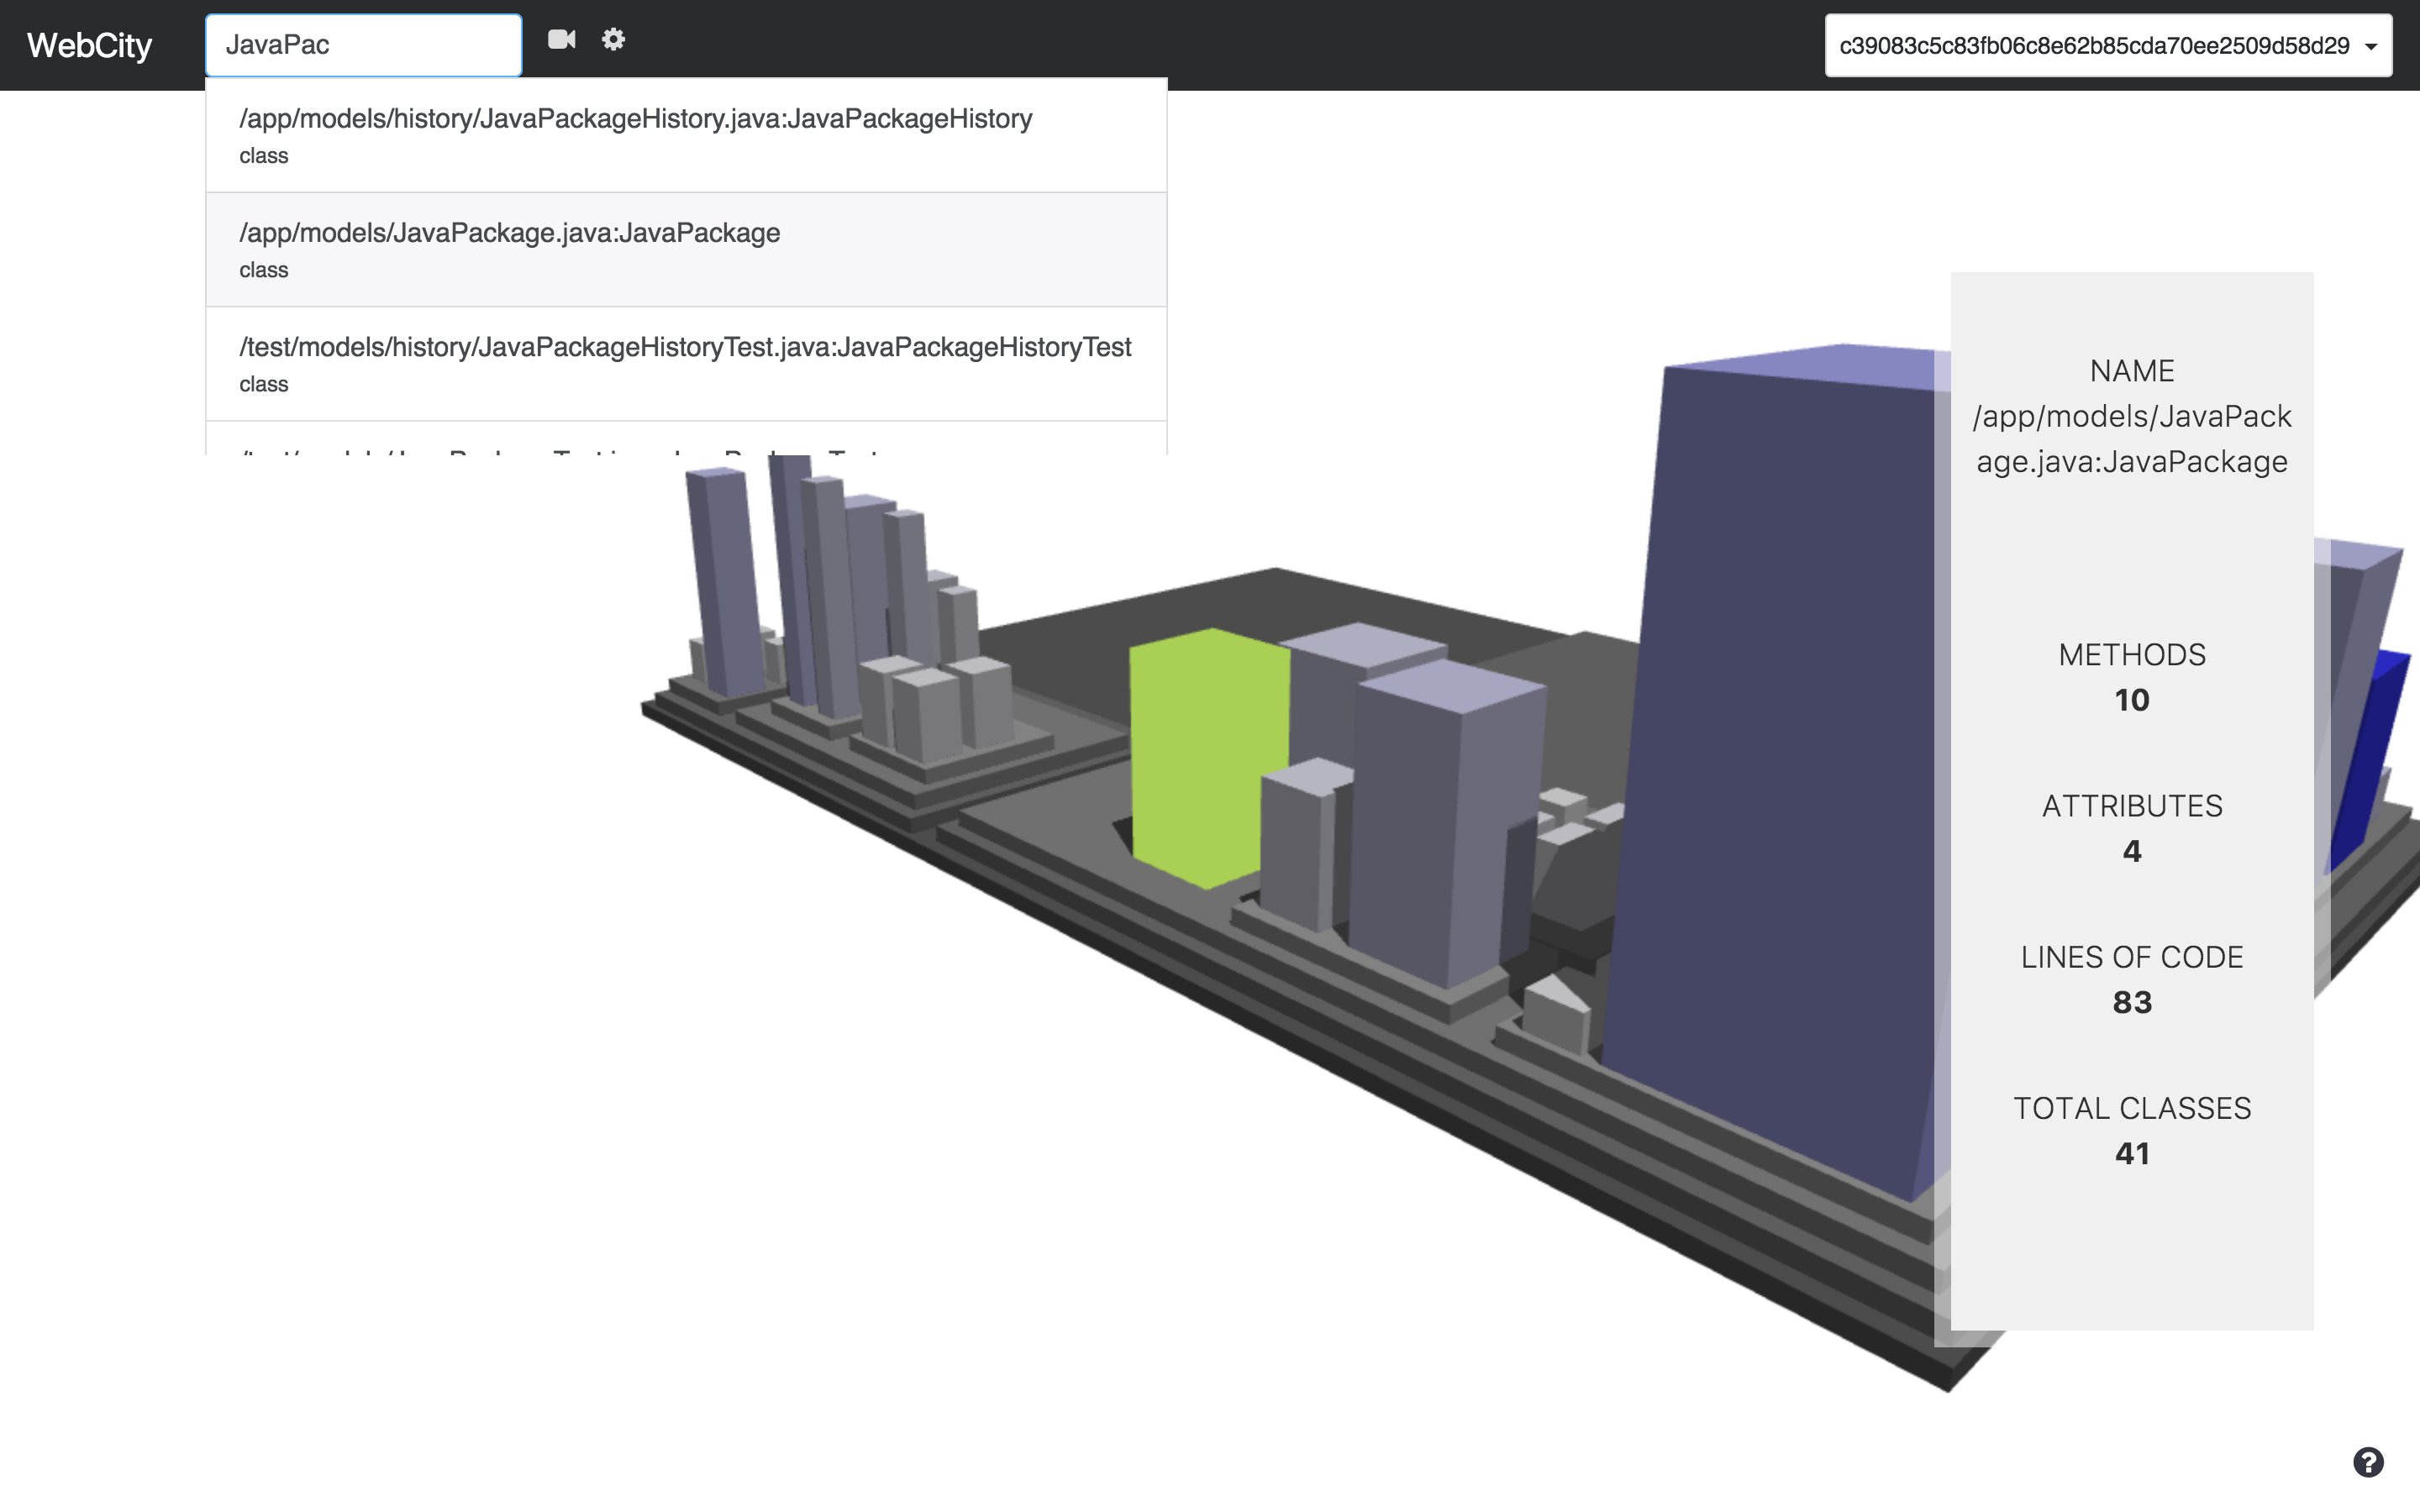
\includegraphics[width=1\textwidth]{pictures/search.png}
\caption{The search functionality}
\label{fig:search}
\end{figure}


\subsubsection{Tag} \label{Tag}
Once we have found the class or package that we were looking for, we might want to be able to move around without losing track of it. We provided a feature to tag the elements
that we are interested in; pressing ``p'' while the cursor hovers an element will change its color to make it more recognizable, and it will keep the information of element on the screen
while we move around. Tagging an element twice or tagging somewhere else will result in the current element being untagged.
Figure \ref{fig:tag} shows the tagged building highlighted in orange, with its information always on screen.

\begin{figure} [H]
\centering
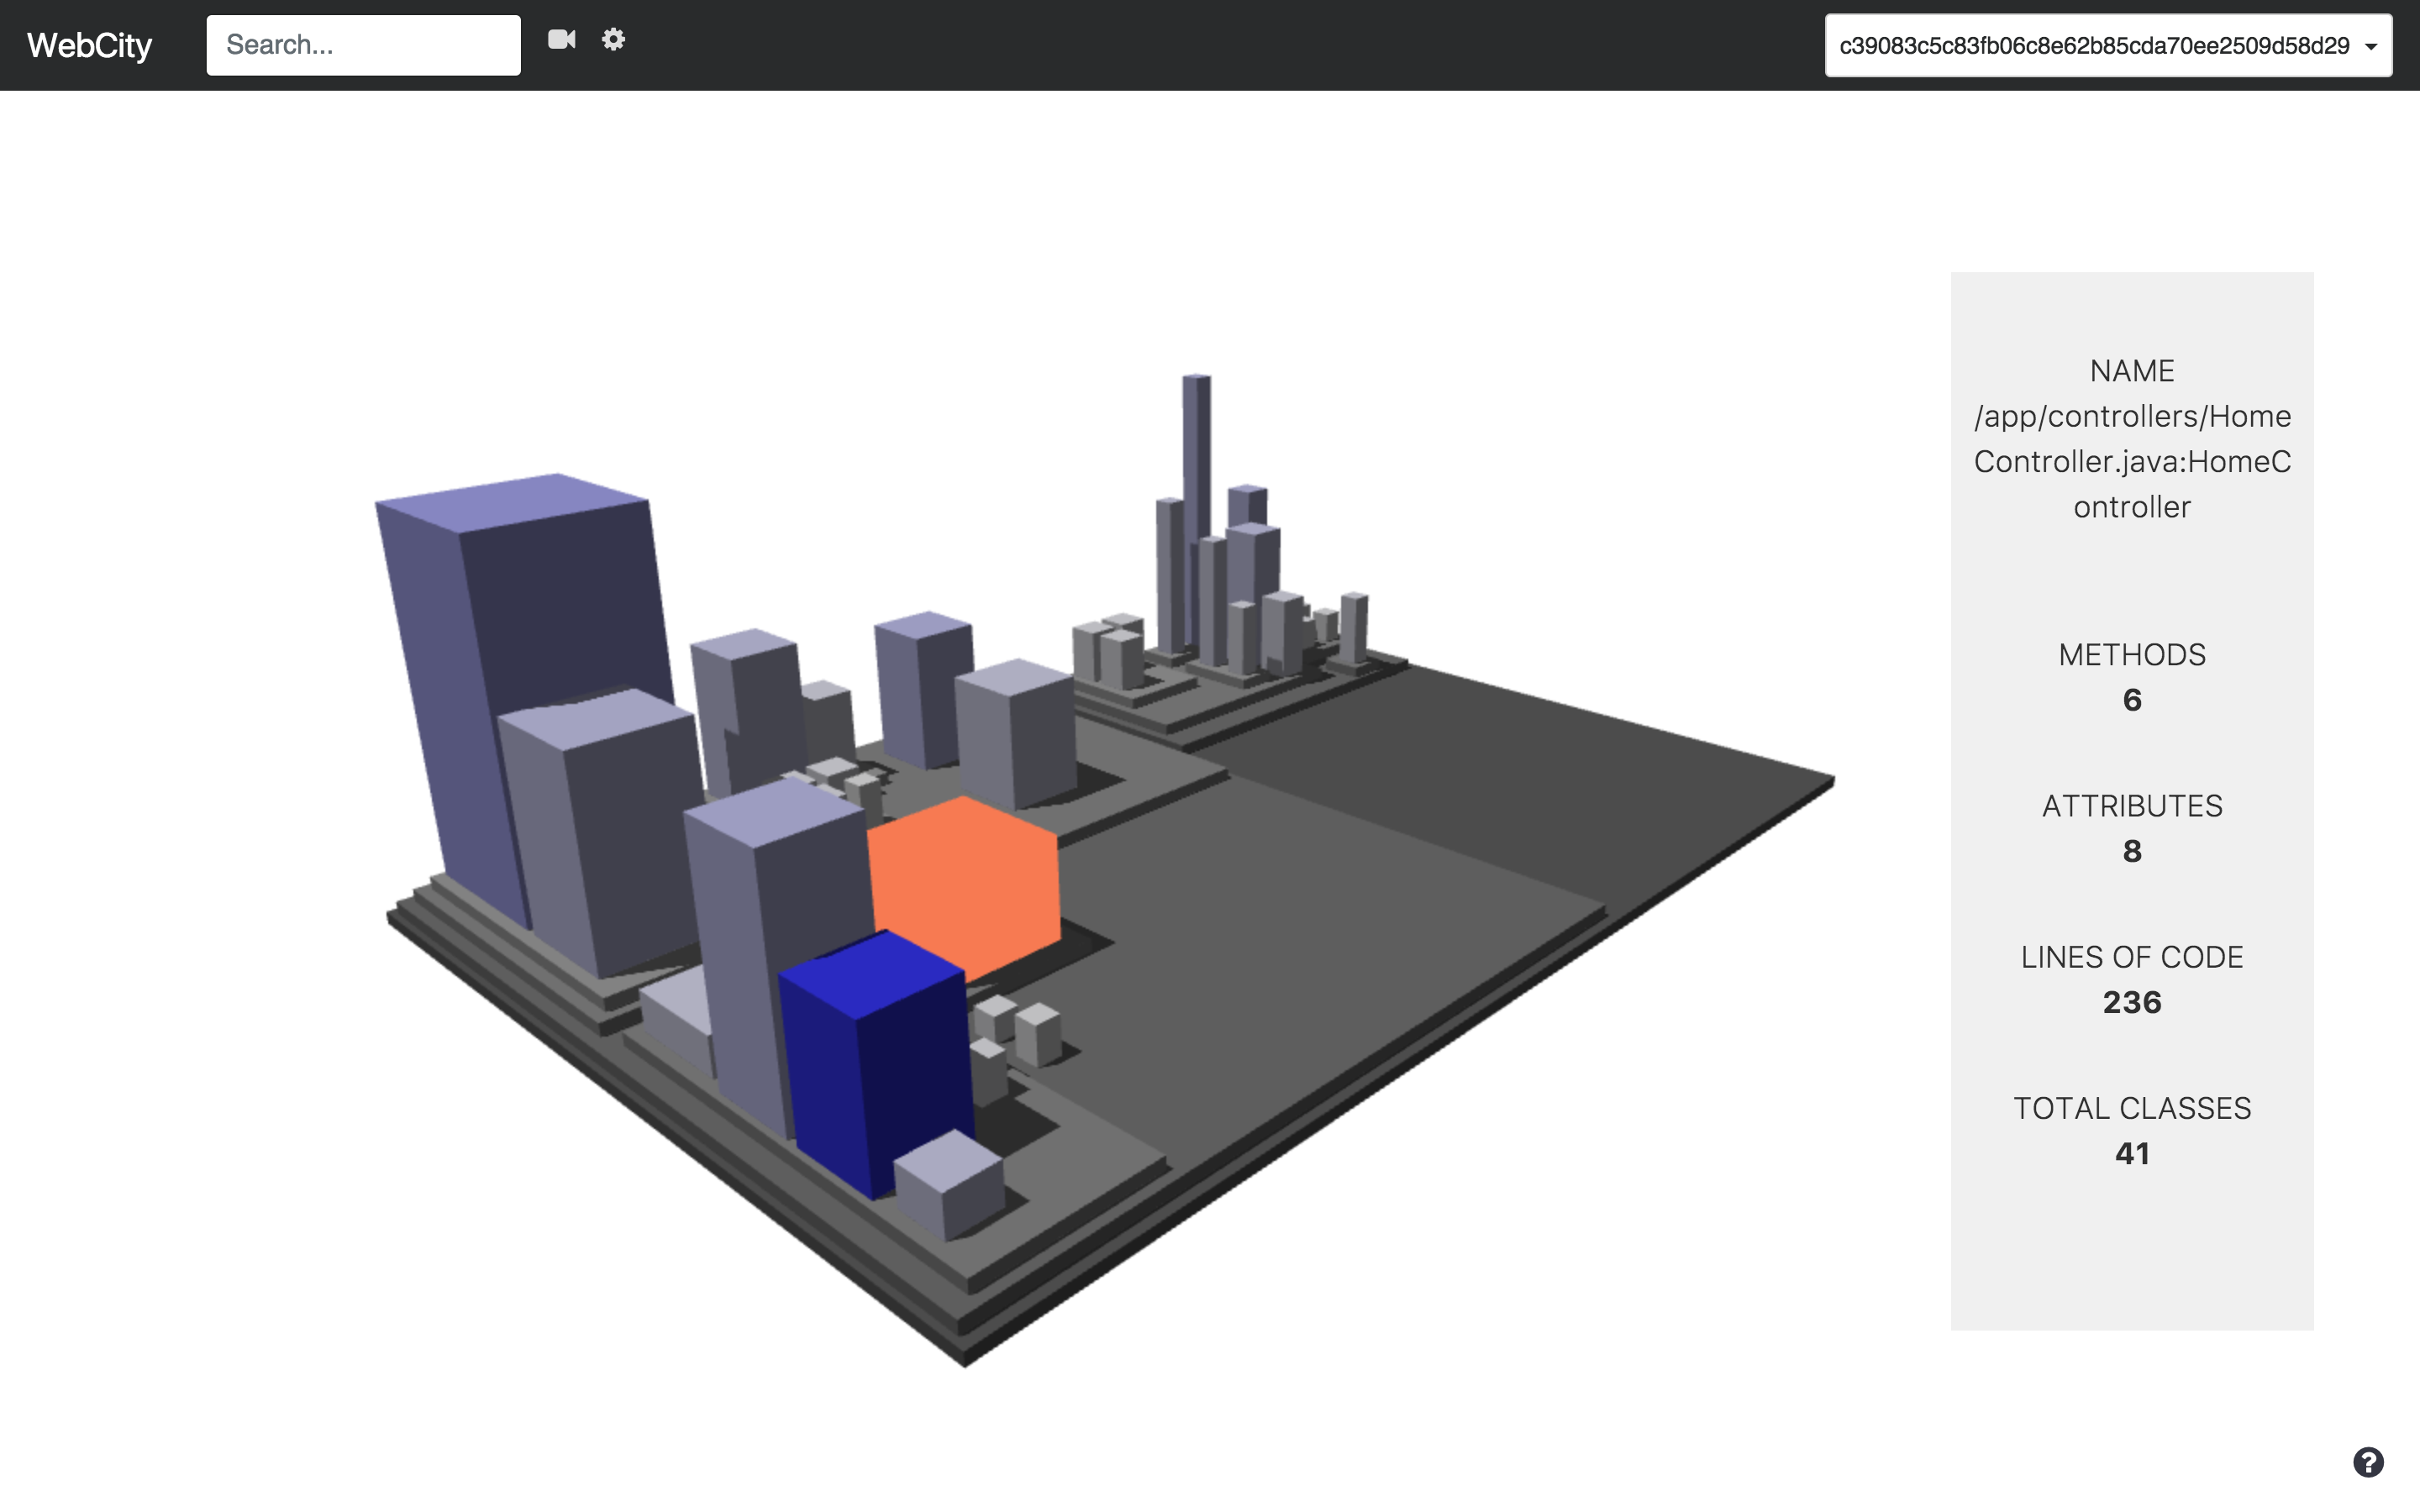
\includegraphics[width=1\textwidth]{pictures/tag.png}
\caption{An example of tagging}
\label{fig:tag}
\end{figure}

\subsubsection{Source code} \label{Source code}
While seeing the statistics on screen of the package or class that we are currently hovering can already give us a lot of information about it, sometimes the user might want to go more in detail and want to go look at the specific implementation of this element.

Our application allows the user to see the source code of the classes or the contents of the packages he's hovering. To do this, we simply have to left click the element while pressing the alt modifier; this will open a new tab or window at the address of GitHub that points to the specific element that we have clicked, at the version that we were visualizing in our app.

\subsection{3D navigation} \label{3D navigation}
Because of the 3D nature of the visualization, it is important for the user to be able to navigate freely around the city. While this problem does not emerge with 2D models, in the 3D case it is apparent that a good
degree of mobility and freedom are necessary, to be able to see the city from different perspectives and look for specific elements; a lot of information could be lost in the 3D model if we would not allow to freely navigate the city.


\subsubsection{Pitch and yaw} \label{Pitch and yaw}
The user can keep pressed the left click and move the cursor to orbit the camera around the city. Moving the cursor horizontally will rotate the city on the xy plane (with respect of our current position), while
moving the mouse vertically will rotate it around the yz plane.

\subsubsection{Pan} \label{Pan}
Holding down the right click and moving the cursor will result in a pan action, which means that the city will move around following the cursor, but it will not rotate. This will also change the target of the camera,
 which is the point where the camera is looking at and also the center of the rotation axes.

 \subsubsection{Zoom} \label{Zoom}
Using the scroll wheel the user can zoom in or out of the visualization, getting closer or further away from where the camera is currently pointing at.

\subsubsection{Size scaling} \label{Size scaling}
Clicking on the cog icon on the header bar, the user can open a tab with three input fields, each one of which can be used to set a size parameter of the visualization:

\begin{itemize}
\item \textit{Padding}: the amount of padding to be inserted between each package and between the neighboring classes in a package.
\item \textit{Minimum classes size}: the minimum size to be given to a class, so that classes that have no methods, no attributes or none of either can still represented instead of being invisible.
\item \textit{Package height}: the minimum height of a single package.
\end{itemize}

These values can be set (or left blank if we don't want to change some of them) so that we can decide how the visualization should be scaled. Note that the final object is scaled before being drawn, so very big values may give similar visualization if the ratios between the sizes are similar.

Take into account that the positions of classes or packages may change depending on the sizes that are given by the user. This is because when, for example, we increase the padding, a class that is in a very deep recursive position will have to be translated more than a class that that is not as deep in the recursion tree, because for each extra level of recursion, its elements are shifted by the extra padding. If we were only increasing the sizes of the paddings, this could be fine: but if we decrease them, and maybe also change the settings at the same time, it could happen that suddenly a package doesn't have enough space anymore in its old position: this is why we may have to reposition some elements during these resizing transformations.

\begin{figure} [H]
\centering
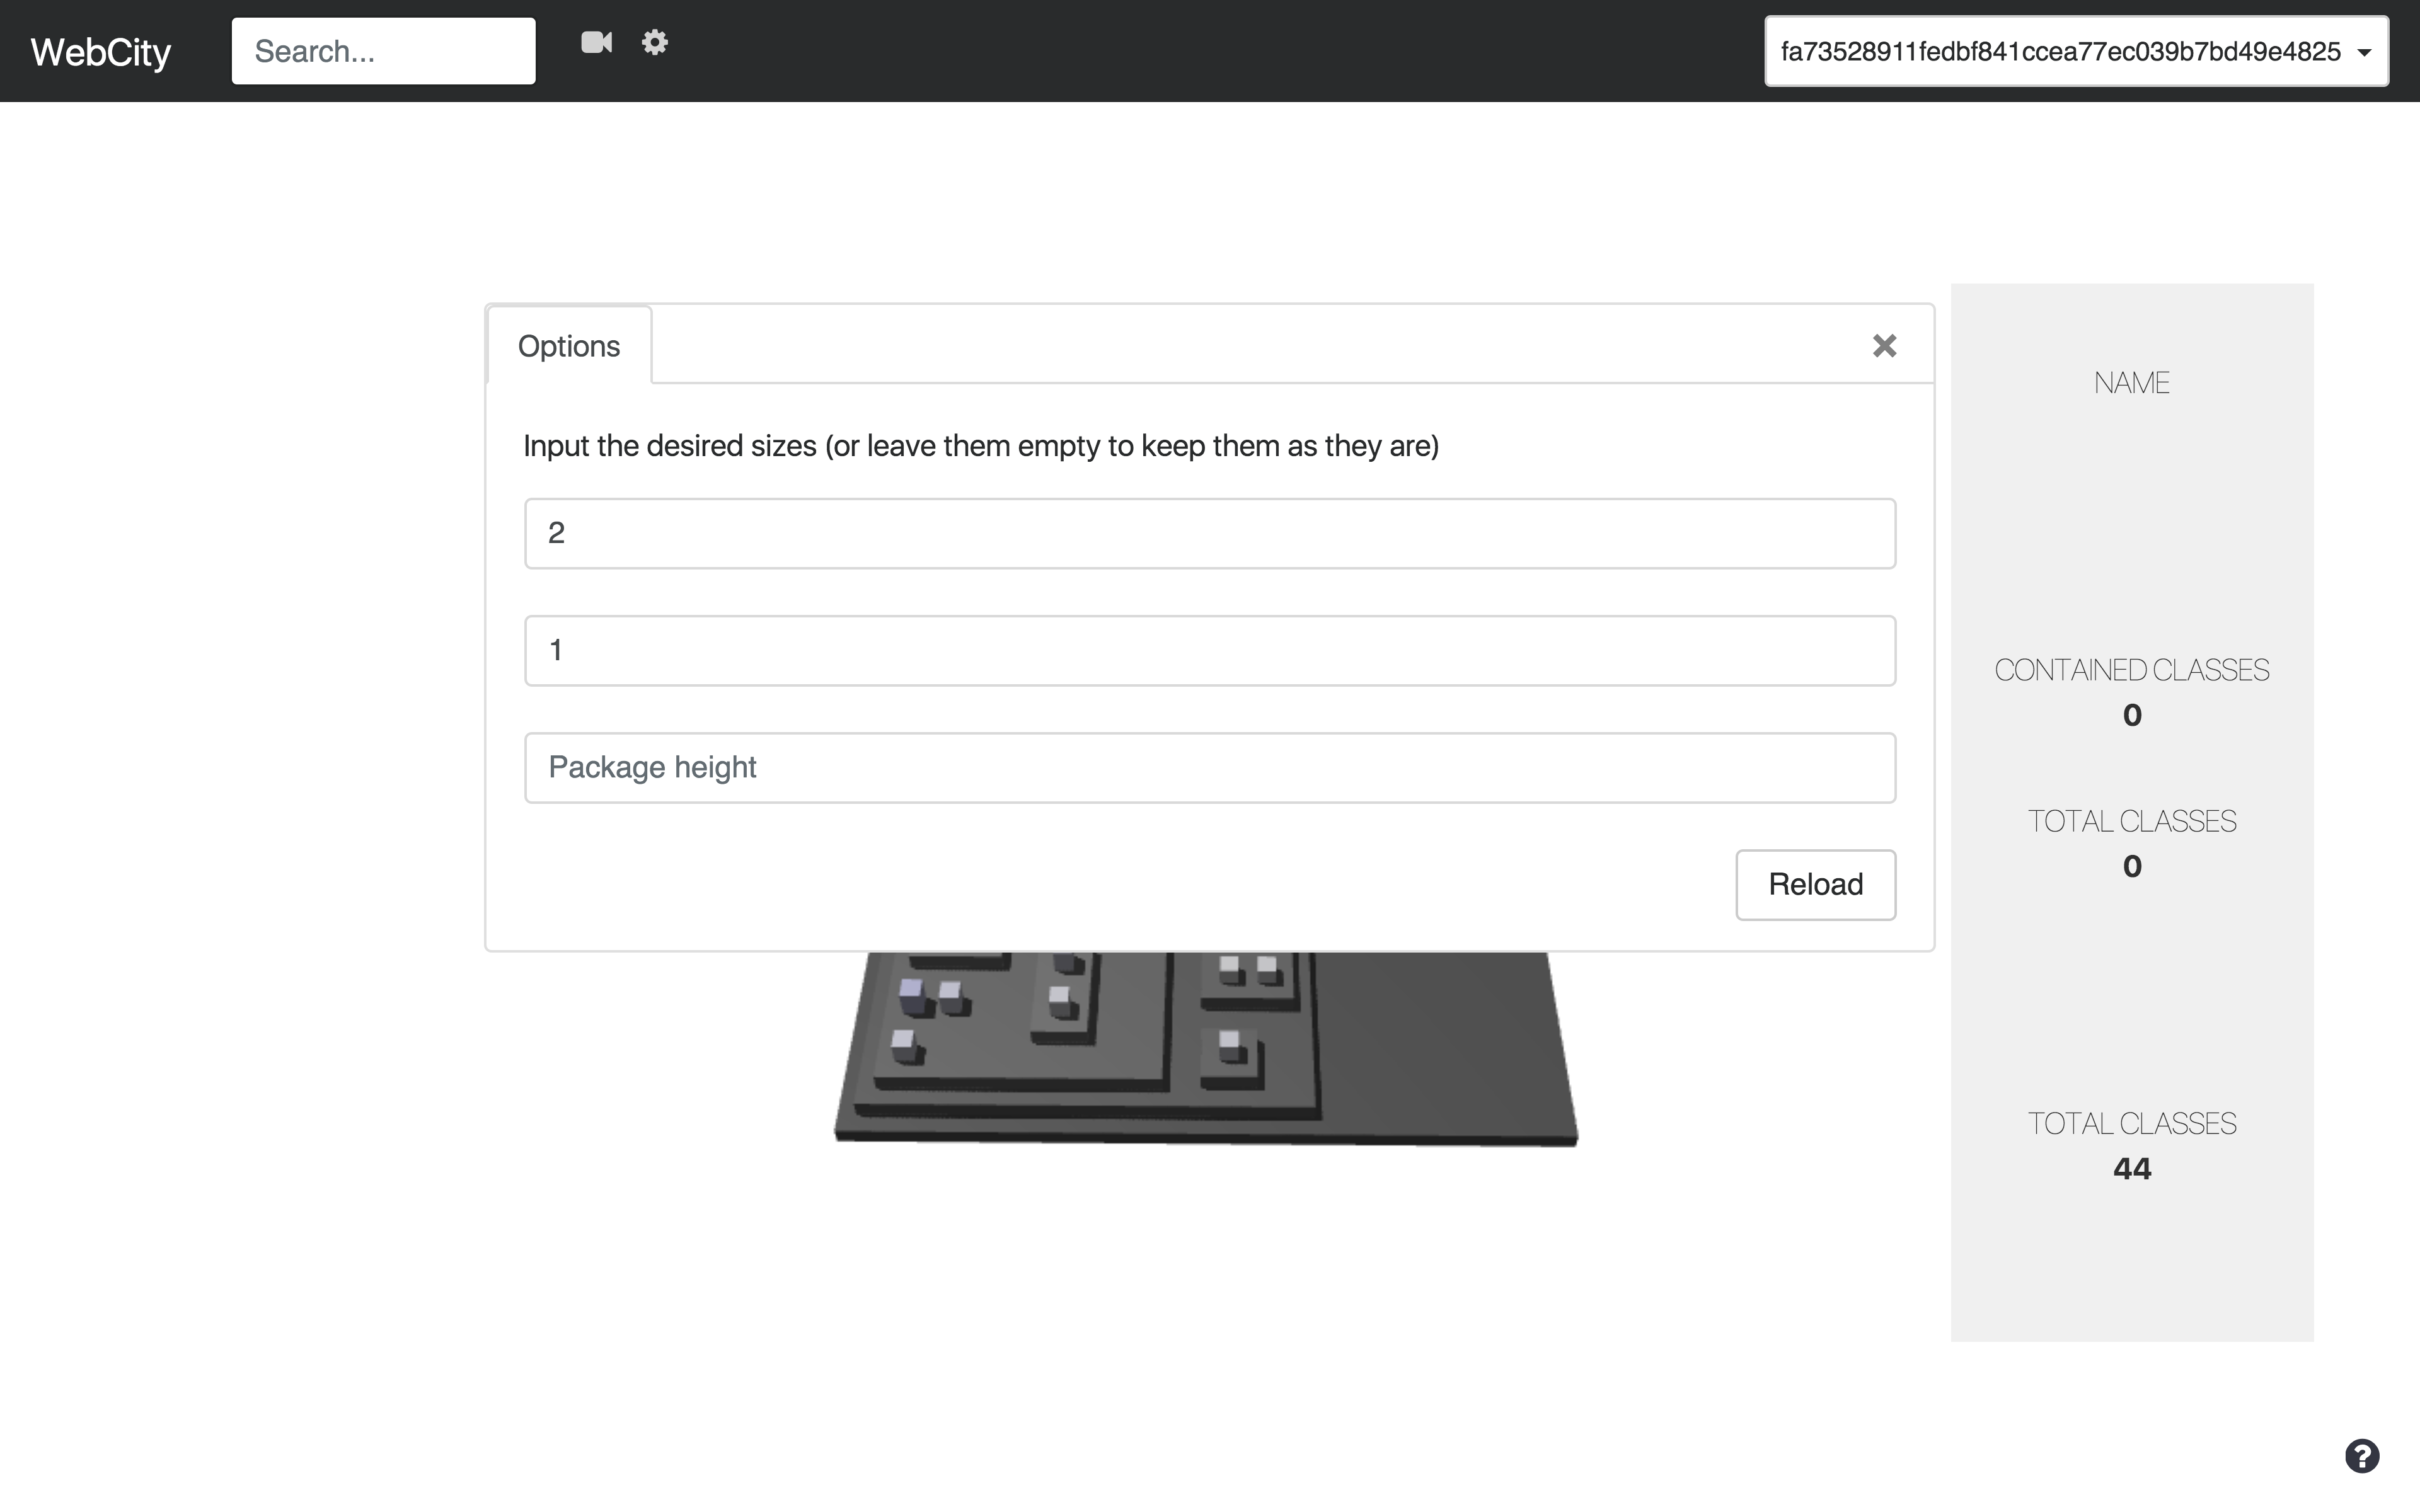
\includegraphics[width=1\textwidth]{pictures/sizing_card.png}
\caption{The options to set the sizing of the visualization}
\label{fig:sizing}
\end{figure}

\begin{figure}[H]
  \centering
  \begin{minipage}[b]{0.49\textwidth}
      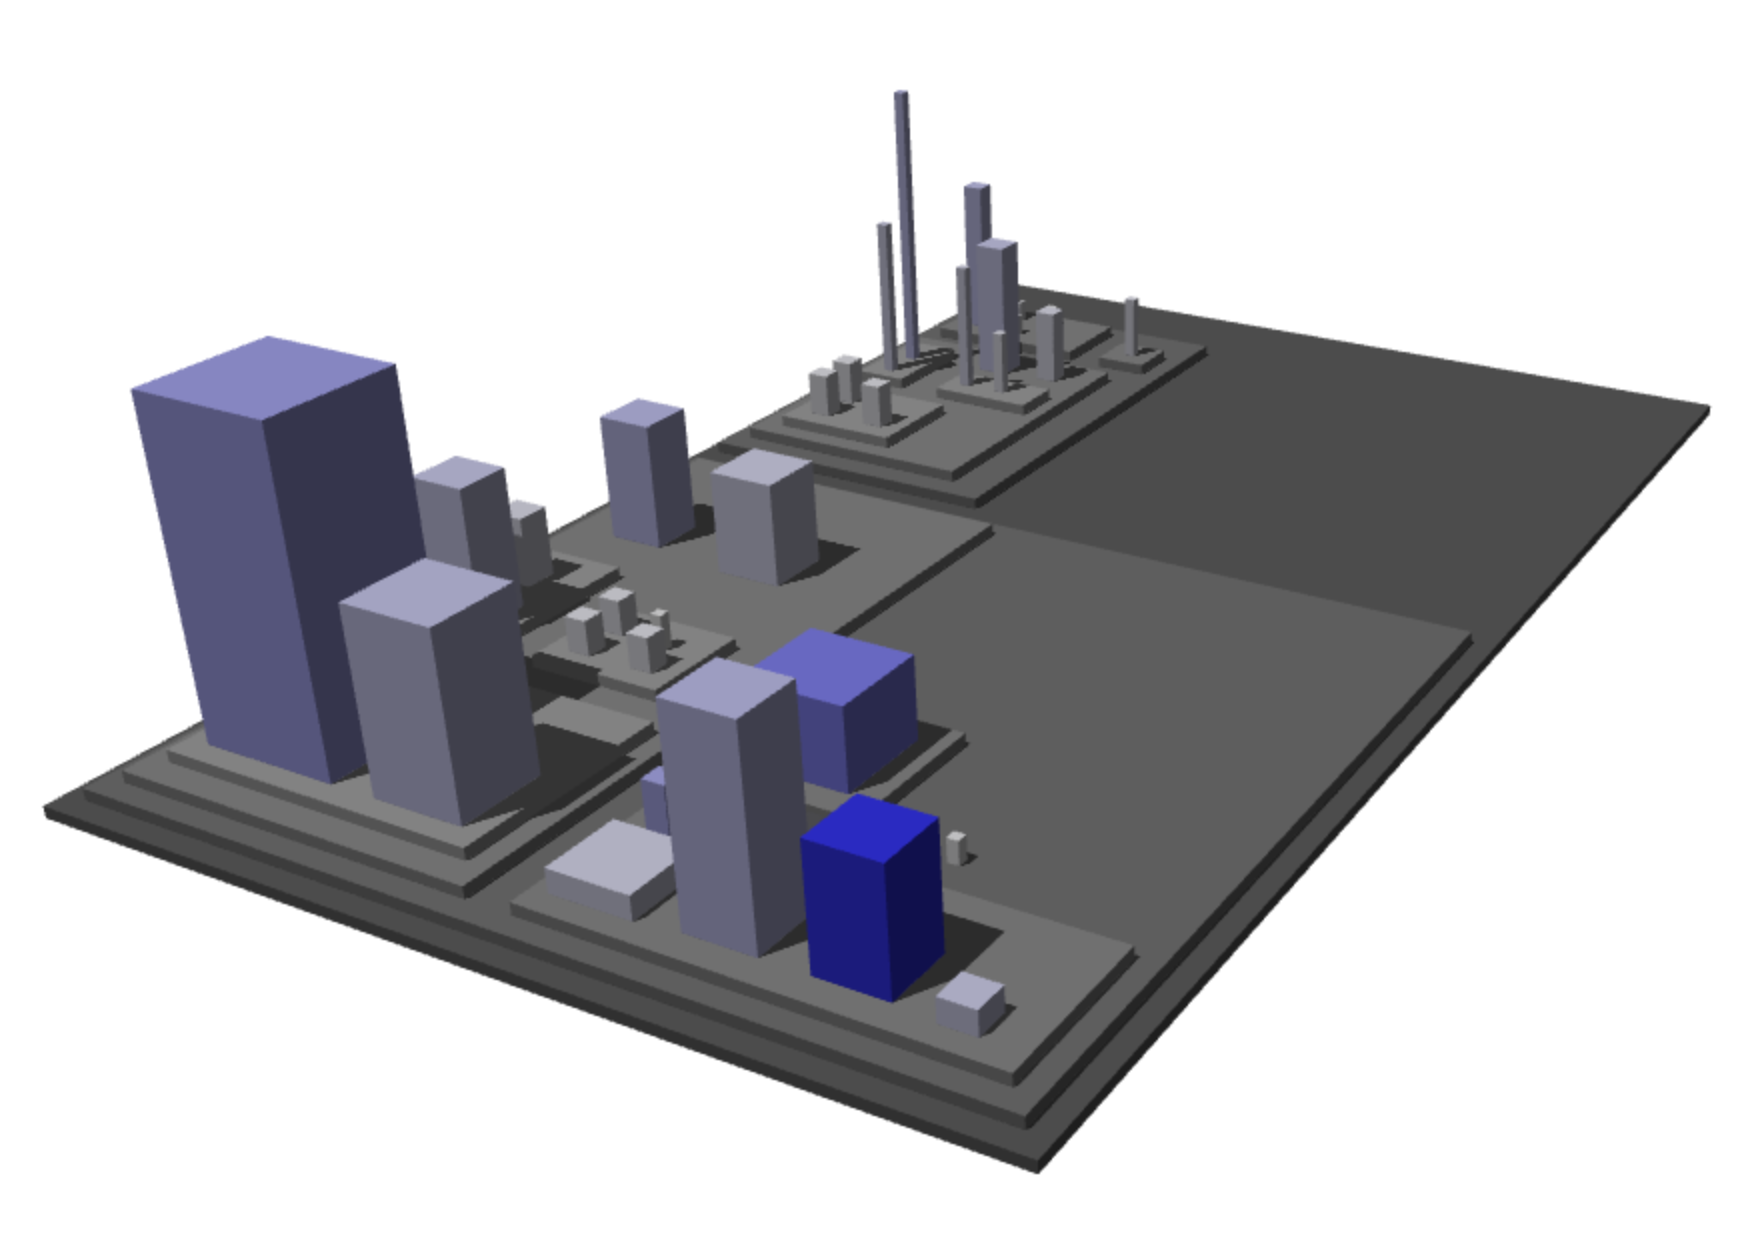
\includegraphics[width=1\textwidth]{pictures/small.png}
      \caption{A small minimum class size}
      \label{fig:sizes small}
  \end{minipage}
  \hfill
  \begin{minipage}[b]{0.49\textwidth}
    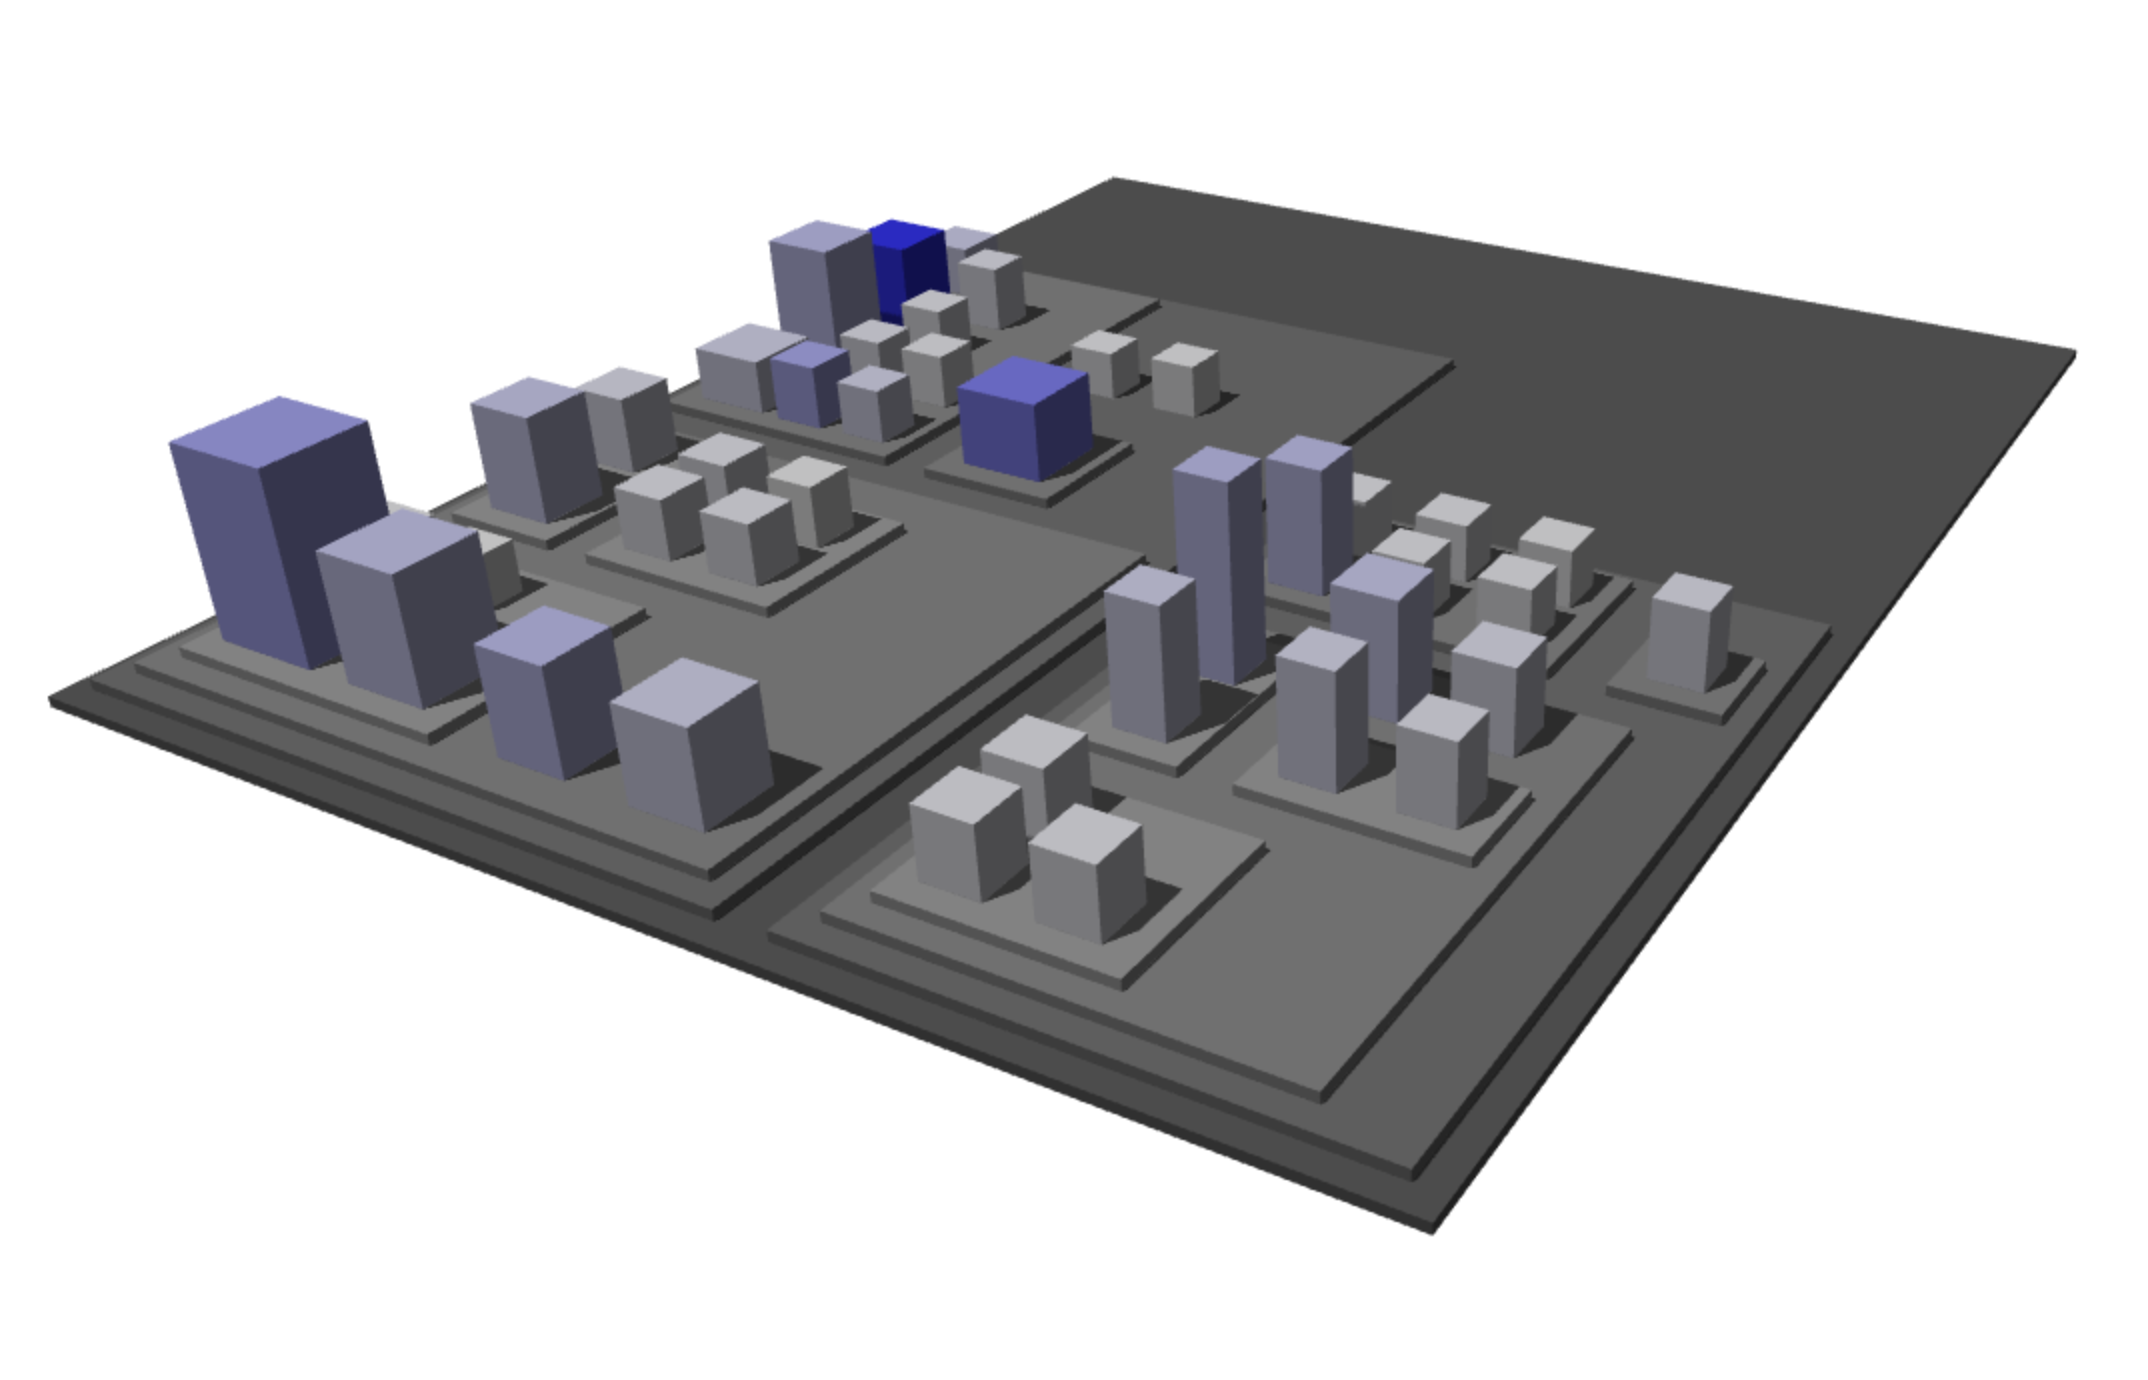
\includegraphics[width=1\textwidth]{pictures/big.png}
    \caption{A bigger minimum class size}
    \label{fig:sizes small}
  \end{minipage}
\end{figure}

\subsubsection{Versions navigation} \label{Version navigation}
For WebCity we decided not just to display a static visualization of a repository in a specific version. Instead, we
decided to add a feature that allows the user to go through the different versions of the repository, going through the history and the evolutionary process of the repository.

 We have added a dropdown on the right of the header, where the user can select the version he wants to see. The app will then update the visualization,  keeping the positions of the elements that did not change to avoid disorientating the user, but at the same time adding, removing or updating the classes and packages according to the files and metrics that were present in that specific version.

 \begin{figure} [H]
 \centering
 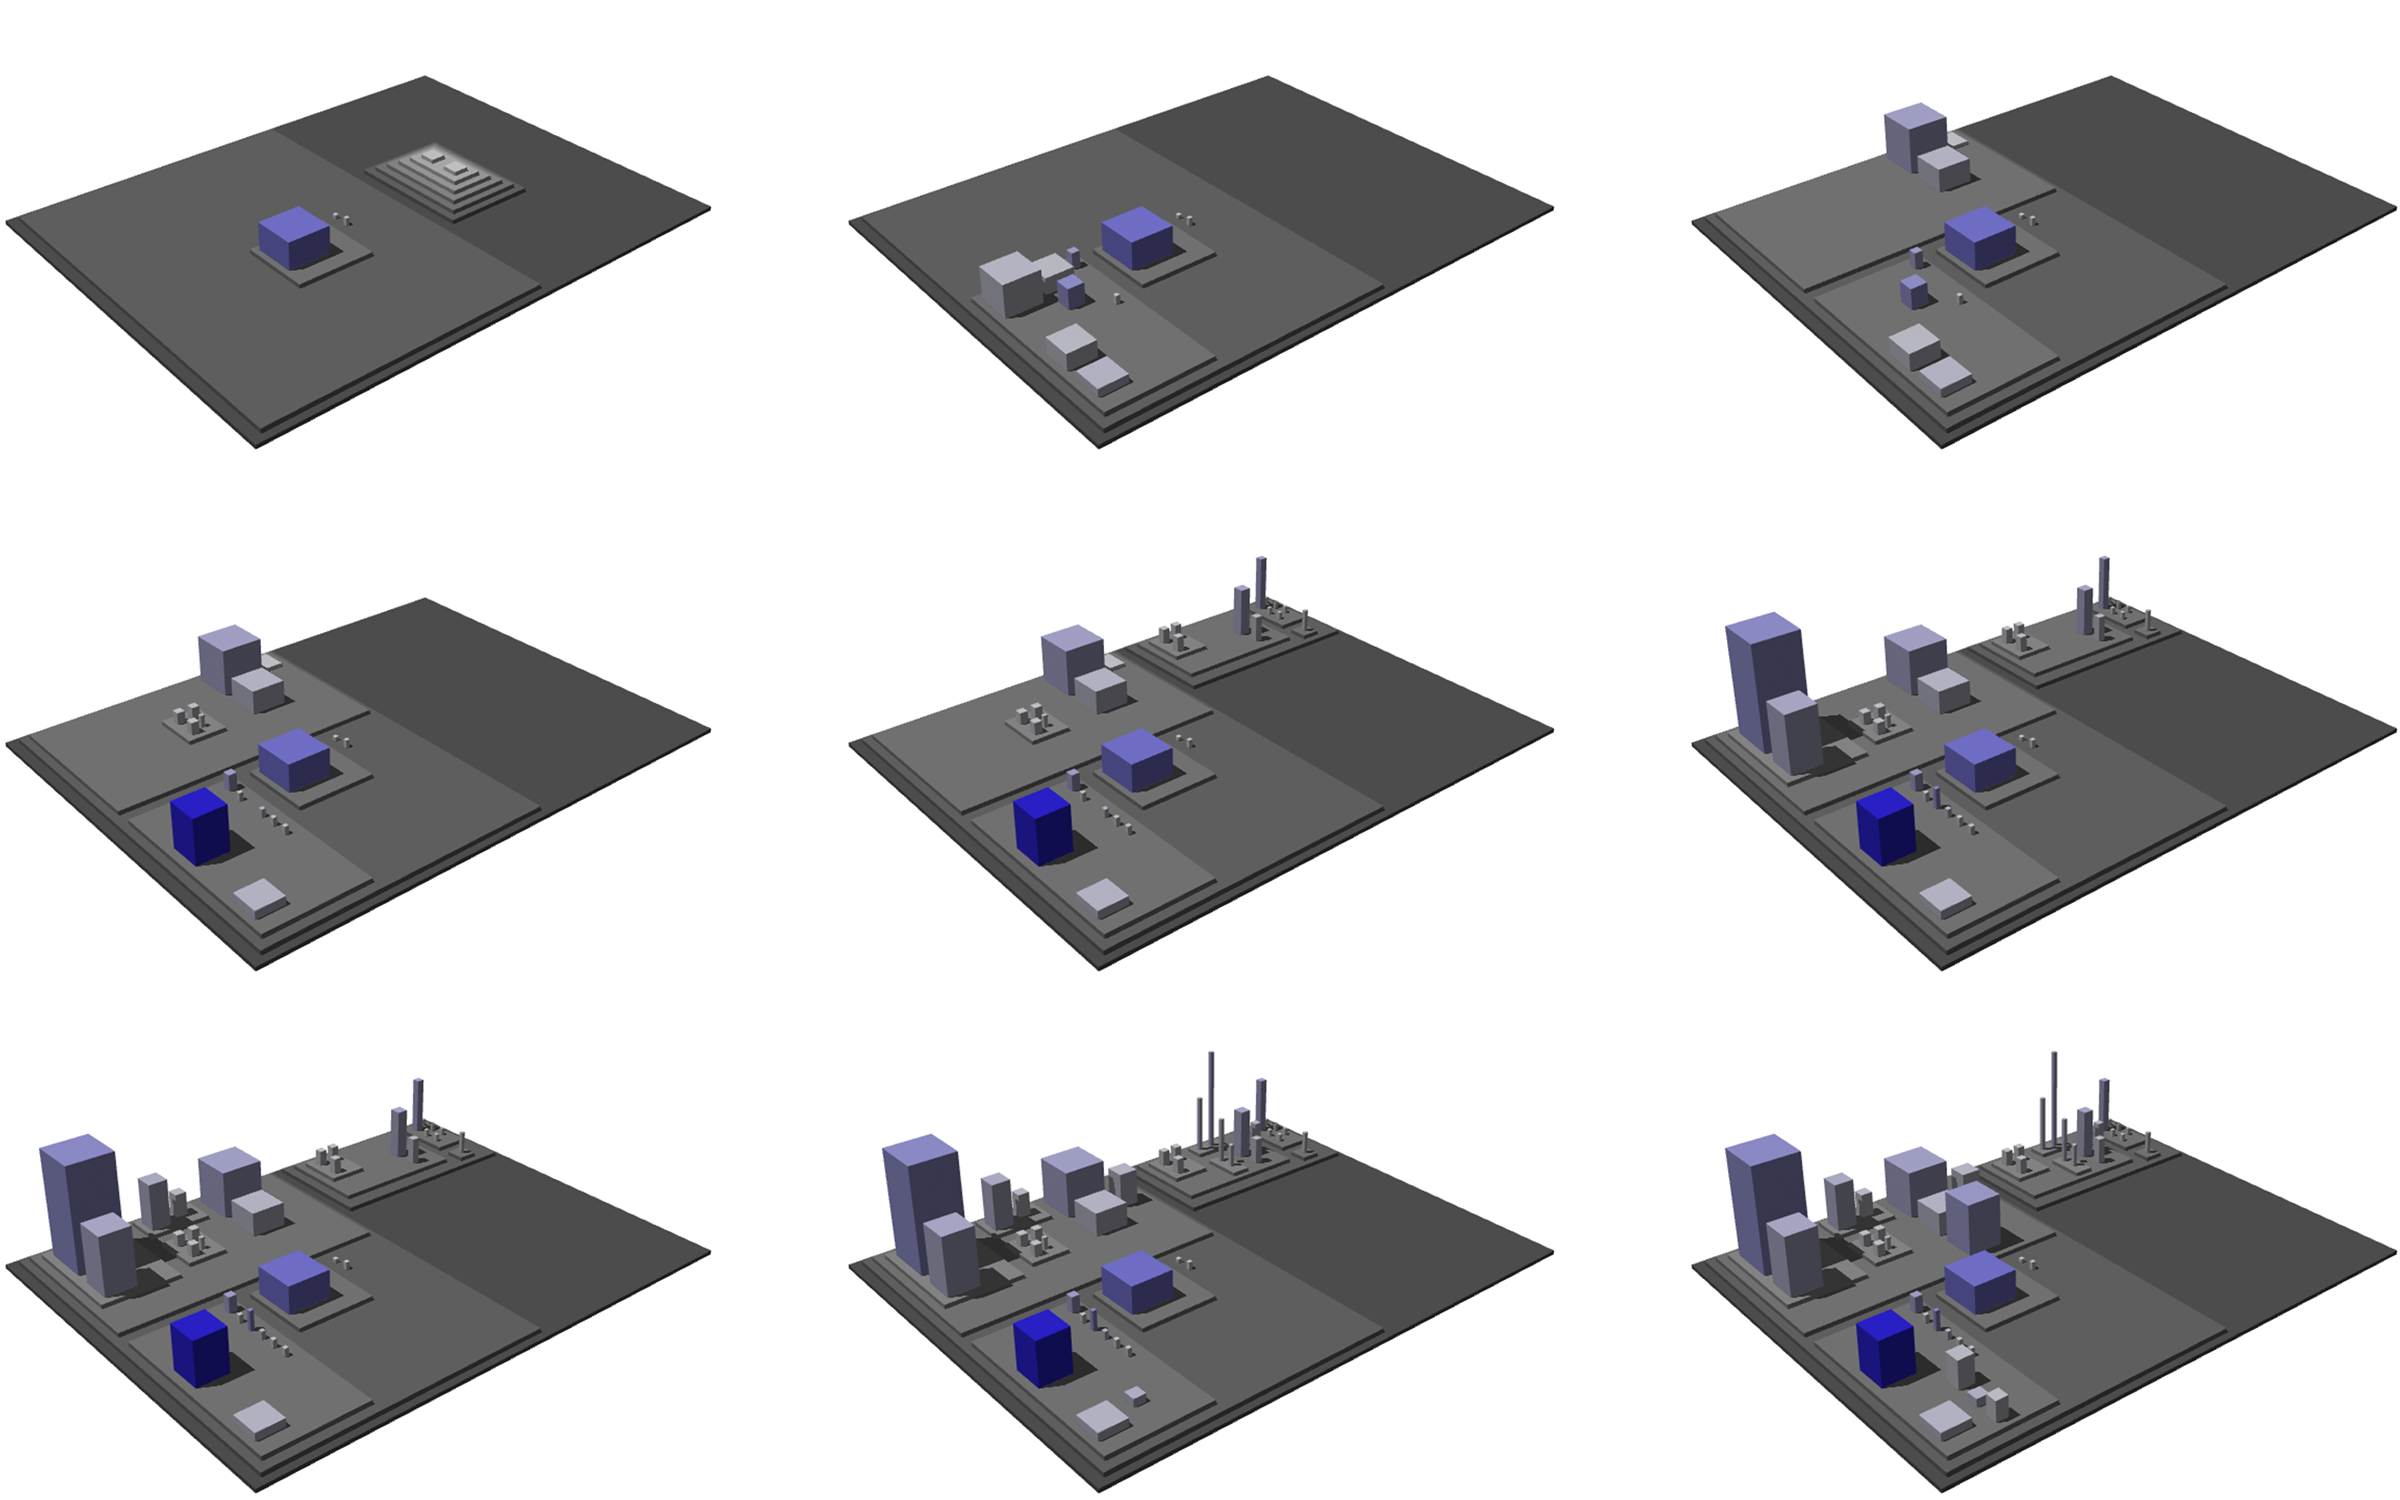
\includegraphics[width=1\textwidth]{pictures/evolution.png}
 \caption{The evolution of WebCity over time}
 \label{fig:evolutionq}
 \end{figure}

\pagebreak

\subsection{Video generation} \label{Video generation}
Since in WebCity we have added the functionality to visualize and navigate the history of the repository through its list of commits, we thought that it might have been interesting to be able to produce something more than just a screenshot, that allows to capture the evolutionary nature of the repositories.

We have therefore implemented a video generation feature. By clicking on the camera icon on the header bar we can select a starting and ending commit for the video, alongside the desired resolution of the video. When we click record, the application will go through the commits between the starting and ending commits that we chose, taking a screenshot of every version, and at the end it will return a generated .mp4 video, having a screenshot of a version for each frame.
There is also an ``orbit'' checkbox: when it is checked, the camera will move on a circumference around the visualization while the screenshots of the versions are being taken, generating a video where user's point of view will be orbiting around the city while it evolves.


\begin{figure} [H]
\centering
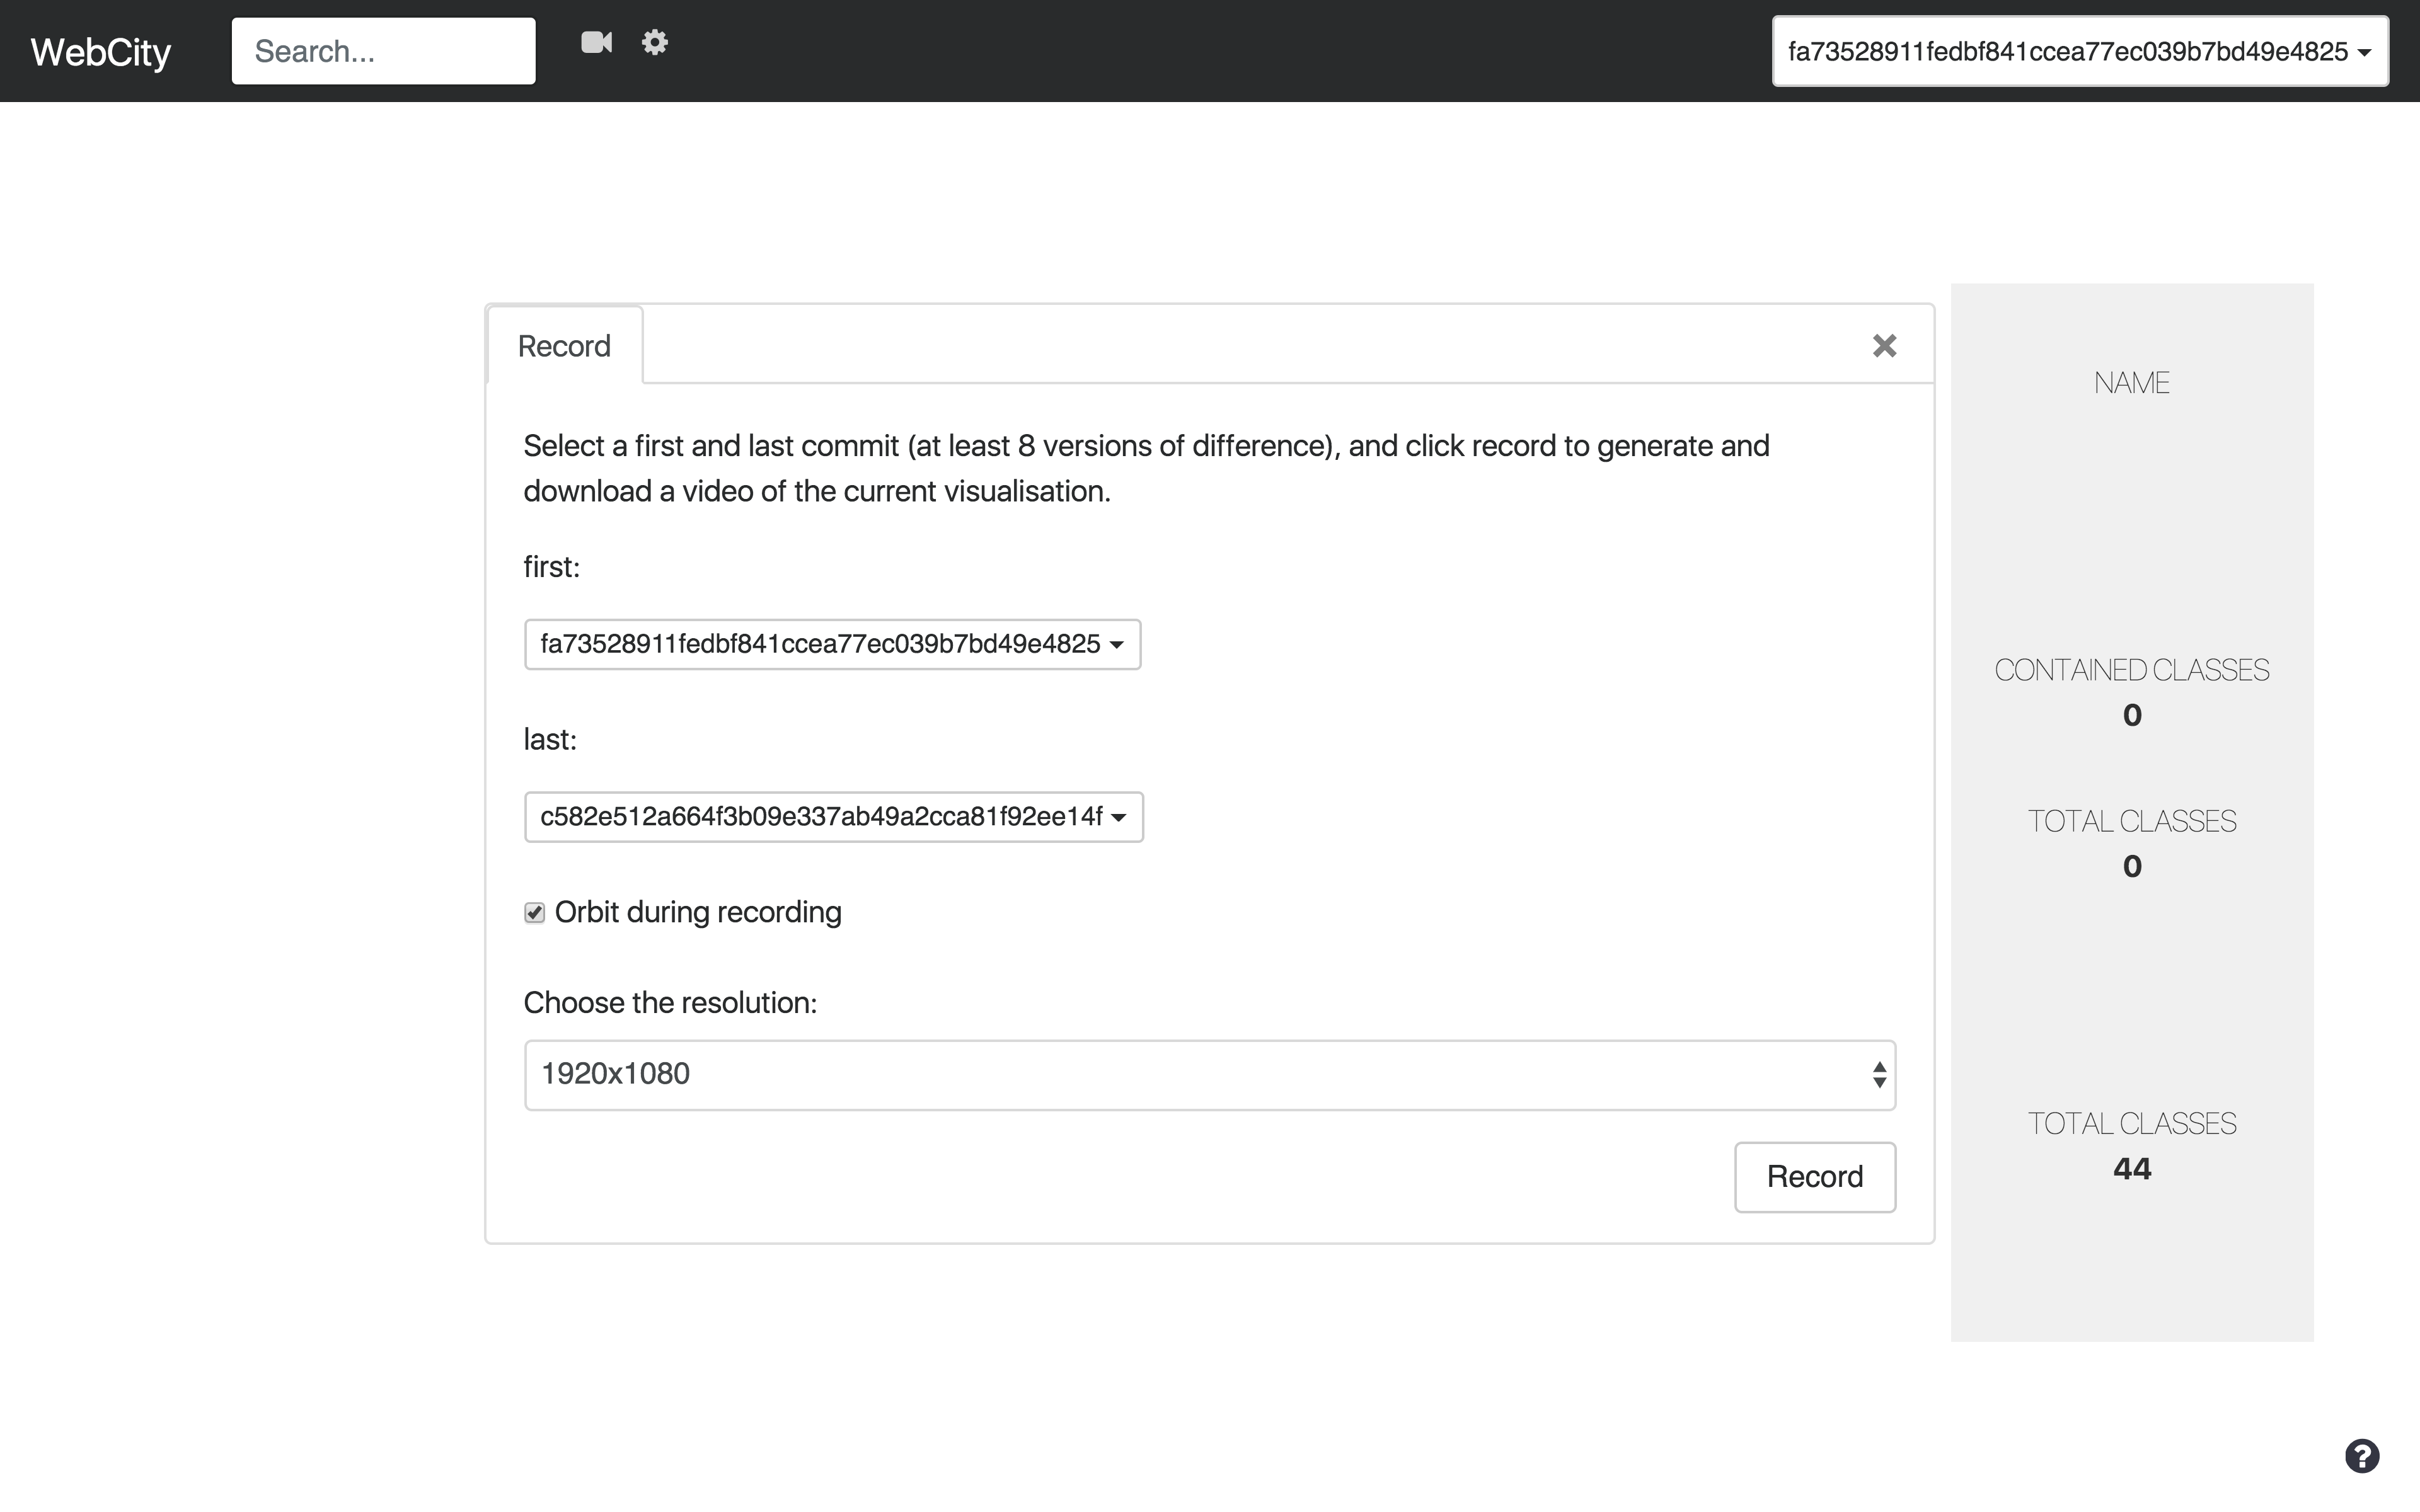
\includegraphics[width=1\textwidth]{pictures/record_card.png}
\caption{The options to generate the video}
\label{fig:record}
\end{figure}

\subsubsection{Implementation} \label{Implementation}

To produce the final .mp4 video we split the process into two parts.
The first part takes care of taking the screenshots of all the versions that the user wants to have in the video. To do this, we use a Javascript function that takes care of selecting automatically the versions, taking a screenshot of the canvas, and then changing to the next version until we have all the pictures we need.
Once we have collected our array of screenshots, we use a version of FFmpeg compiled to Javascript to take care of merging the images. Because of the linear nature of Javascript the compiled version of FFmpeg.js is not very fast, but with some optimizations, such as using web workers to make multiple smaller videos and merging them together at the end, we were able to improve its performance.

\subsection{Architecture} \label{Architecture}

Before we start parsing version and packing rectangles, we need to have a model to follow, so that we can store the data in a meaningful and usable way.

When we are parsing, for each Java class we find, we create a JavaClass, which is an abstraction for the class, where we store the minimal information about the class, like its name, its path, and its metrics.

Then for each package we make a JavaPackage, which can contain references to other children JavaPackages or JavaClasses.
On top of this, we have JavaClassHistories and JavaPackageHistories, which represent a list of the versions in which specific packages and classes are present, so that for each class or package we have information on its whole history.

We then have Drawables, which are container classes that extend JavaClasses and JavaPackages with extra information needed for drawing them, such as position and color.

\begin{figure} [H]
\centering
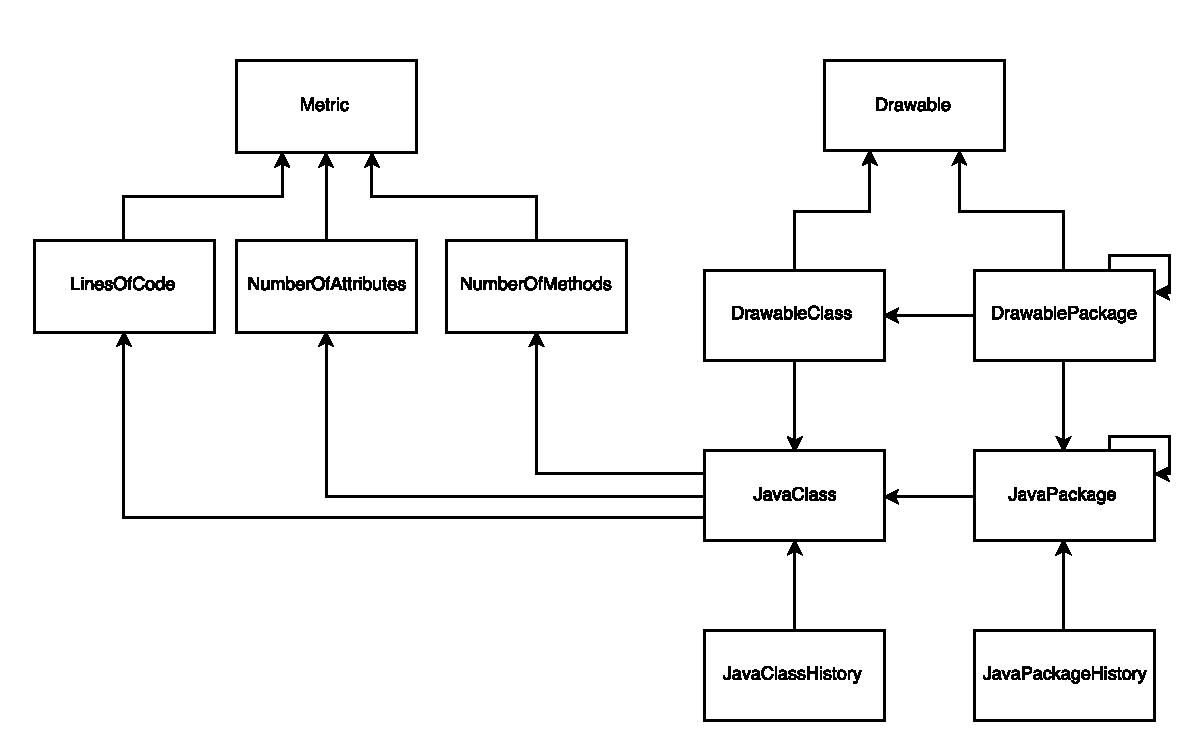
\includegraphics[width=1\textwidth]{pictures/models.pdf}
\caption{Simplified UML class diagram}
\label{fig:UML}
\end{figure}

\subsubsection{Control flow} \label{Control flow}
Figure \ref{fig:flow} shows a simplified diagram of the general flow of the application. The user inputs the URL of a repository, then the server side checks if this specific repository had already been downloaded and parsed; if this is the case, it directly sends back the data for the visualization. If it's a new repository, the server clones it from GitHub, it parses it, it uses the rectangle packing algorithm to find the position of the elements in the visualization, and send the data back to the client to be used for the 3D rendering.

WebCity makes use of various other libraries and technologies that run alongside code written by us to be able to produce the visualizations.

The client side is written in HTML5, CSS3 and Javascript; of the Javascript part, some are external libraries, mainly jQuery, ffmpeg.js (a version of ffmpeg compiled to Javascript) and Three.js, which is the library that then runs WebGL undearneath to make the 3D visualization.

When the user gives the link of the desired repository to be analyzed, on the server side we use jGit to interface with GitHub, and then JavaParser to parse the Java code to gather the data on the system. When this is done, The server side does the calculations using a rectangle packing algorithm to decide where to position the packages and classes with respect to each other. Then the data needed for the visualization is sent back to the client side, which uses Three.js to display the 3D city on the browser.

\begin{figure} [H]
\centering
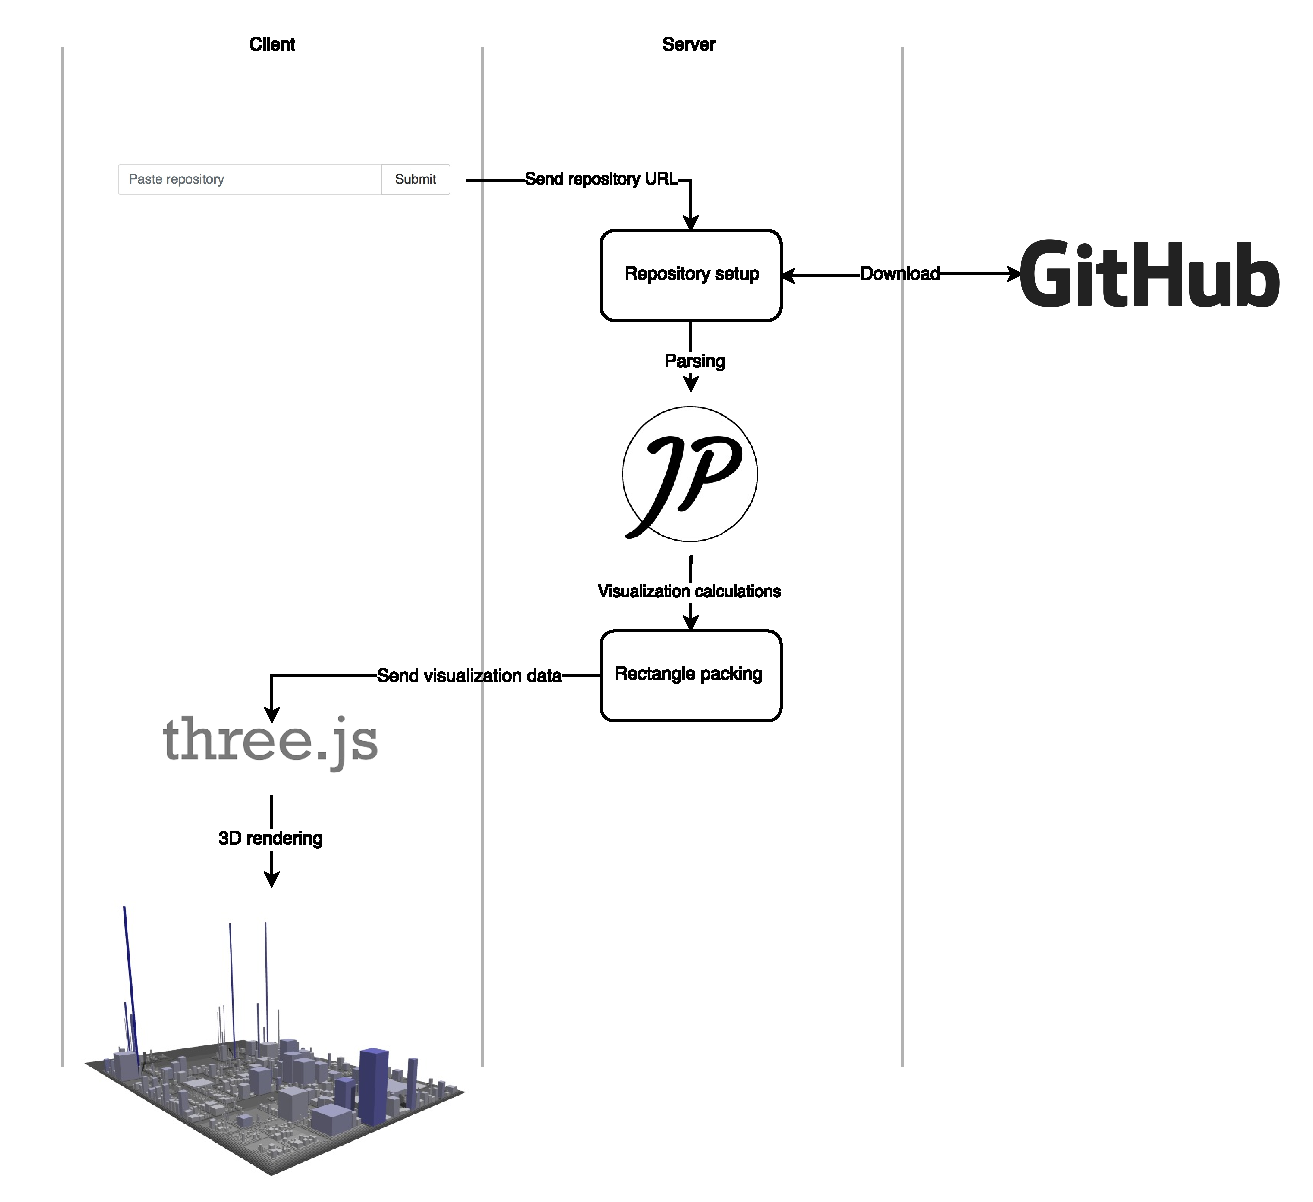
\includegraphics[width=1\textwidth]{pictures/flow.pdf}
\caption{Flow of the application}
\label{fig:flow}
\end{figure}

\subsection{Parsing} \label{Parsing}
If it is the first time that we are visualizing a certain repository, we have to parse every version of the repository to get the necessary information on the code metrics.
The parsing of the Java code is done using JavaParser, a Java library that simplifies the parsing of the repositories by allowing us to go through all the classes and their contents.
For each Java file we find we visit every class contained in it, and get information on their methods, their attributes and their number of lines of code.

The data we collected is used to create objects that represent classes and packages: JavaClass is the abstraction of a Java class, that contains information about its own metrics; then JavaPackage, the abstraction of the package, can contain information about the other elements -- packages or classes -- that are contained inside it.

The parsing can take a long time when both the number of versions and the size of the single versions are big.
It is difficult to improve its performance, because to do the parsing of the files we depend on JavaParser (which is quite fast anyways), and, more importantly, because to parse a version we first have to do its checkout from the local repository, which means that doing the parsing in parallel could not be done in a simple and intuitive way, as we cannot do multiple checkouts at the same time.

\subsection{Rectangle packing} \label{Rectangle packing}
% // cite yuri page\\
Once the server side is done parsing all the versions of the repository, it means that we have gathered the data and the information on the metrics for the whole system, and we are ready to prepare the information that will then be used to generate the visualization. This means that we have to calculate the positions for all the classes and the packages of the system. Since the model we are using is the model of the city, the classes will be represented as buildings where the height is mapped to the Number of Methods and the width and depth of the building are mapped to the Number of Attributes. Since the buildings will all have a square base, we used a rectangle packing algorithm to decide where to position the different classes and buildings relative to each other.

We iterate the packages using a depth first algorithm, and we start placing them at the bottom left corner of the representation, in our case at position (0, 0). We do it recursively with a depth first algorithm because we have to know how much space the children packages occupy before we know how much space we need for the parent.
Once we reach a child package that doesn't contain any sub-package, or if we already placed every children package in this current package, we position the classes that are directly contained in this package. We either pack the classes vertically or horizontally, depending on which makes the bounding box of our current package grow less, to minimize the wasted space and to keep the visualization compact.

\begin{figure} [H]
\centering
\includegraphics[width=.7\textwidth]{pictures/junit4Above.png}
\caption{The rectangle packing of Junit4}
\label{fig:rectanglePacking}
\end{figure}

\subsubsection{Bins} \label{Bins}
The space during the rectangle packing algorithm is handled using \textit{bins}. A bin is a rectangular portion of the canvas, which can be used both to keep track of the space that has already been occupied and to keep track of the empty spaces that we can still use to place packages and classes.

Whenever we place an element in a bin, we divide the remaining space of the bin into multiple possible new bins, and add them to the list of empty bins. When we will be trying to position a new package, we will try to fit it into the smallest bins possible in the list of empty bins, either vertically or horizontally.

Figure \ref{fig:bins} shows three possible open bins in red, blue and green where new packages could potentially be placed in. Figure \ref{fig:binsPlacing} Shows what happens when we place a new element. When the grey package is placed, the blue bin gets removed, and the new red and green bins get created.

\begin{figure} [H]
\centering
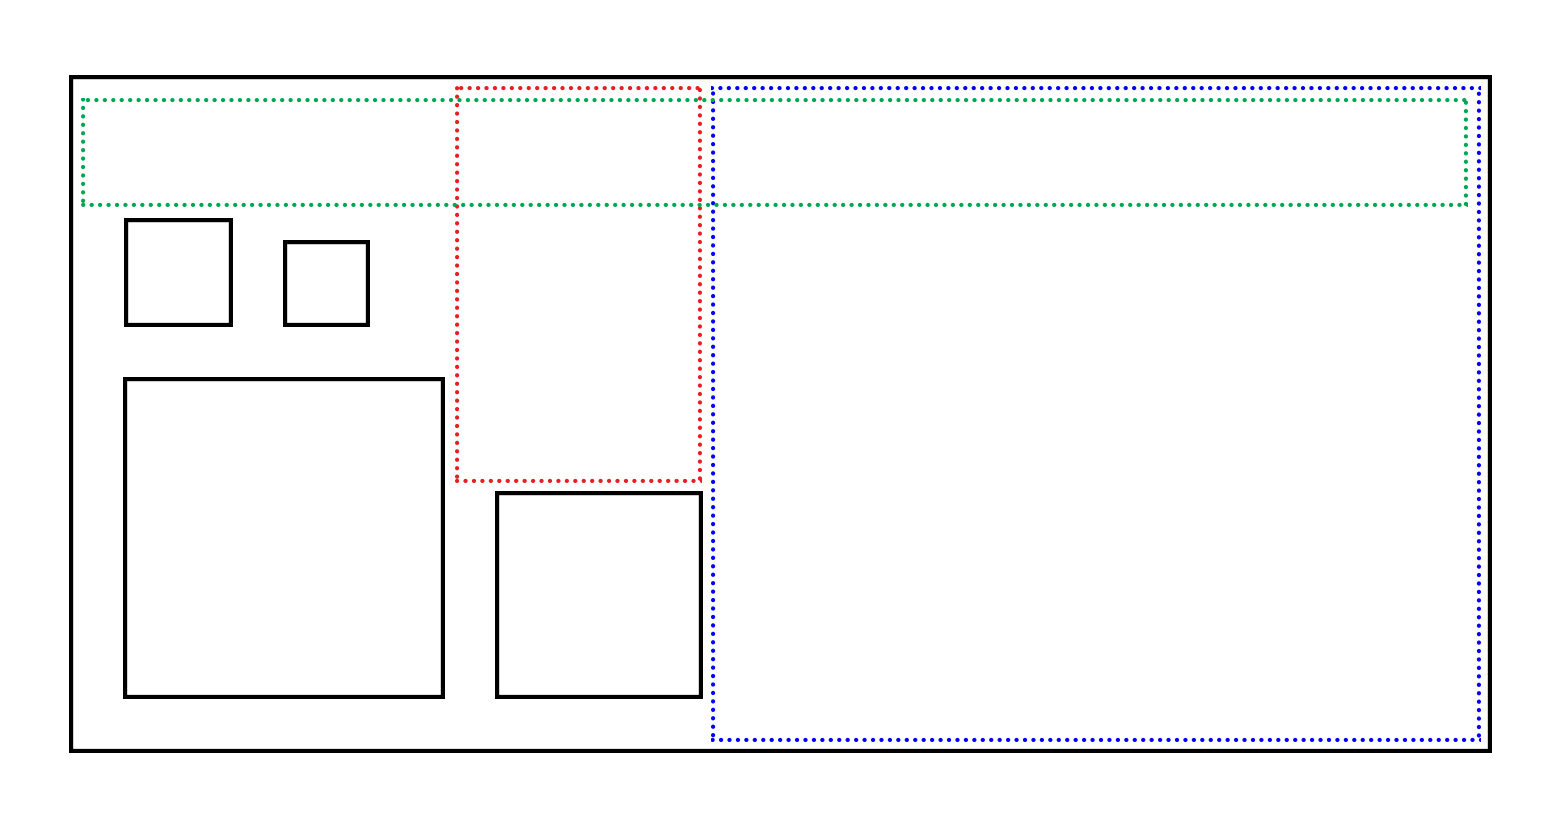
\includegraphics[width=.7\textwidth]{pictures/bins.png}
\caption{Two possible open bins where to place our next element}
\label{fig:bins}
\end{figure}

\begin{figure} [H]
\centering
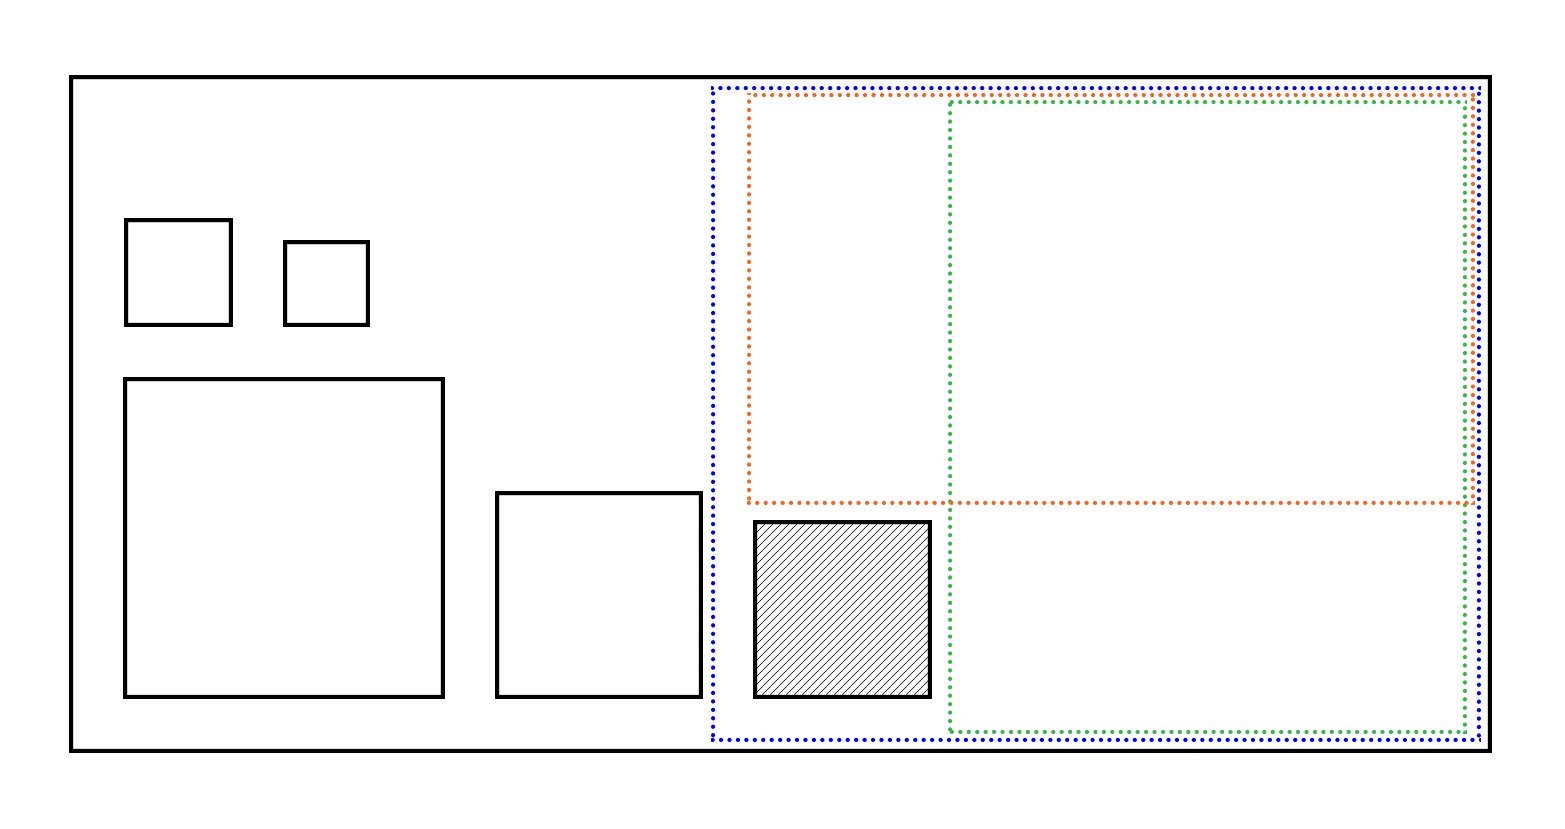
\includegraphics[width=.7\textwidth]{pictures/binsPlacing.png}
\caption{When we position an element, we split the bin we used to create new possible open bins}
\label{fig:binsPlacing}
\end{figure}

\subsubsection{Classes packing} \label{Classes packing}
The rectangle packing algorithm to position the classes inside a package is fairly simple. Once we have found an open bin and we know that we have enough space (vertically or horizontally) to fit all the classes, we start placing them in order of size, from biggest to smallest, one next to each other. Once a row -- or column -- cannot fit another class, we go back at the beginning of the row and we stack a new row on top of it. The padding between the classes and between the classes and the package is the same, and can be set manually by the user.
Figure \ref{fig:classesPacking} shows a simple example of how the final positioning of classes looks like.

\begin{figure} [H]
\centering
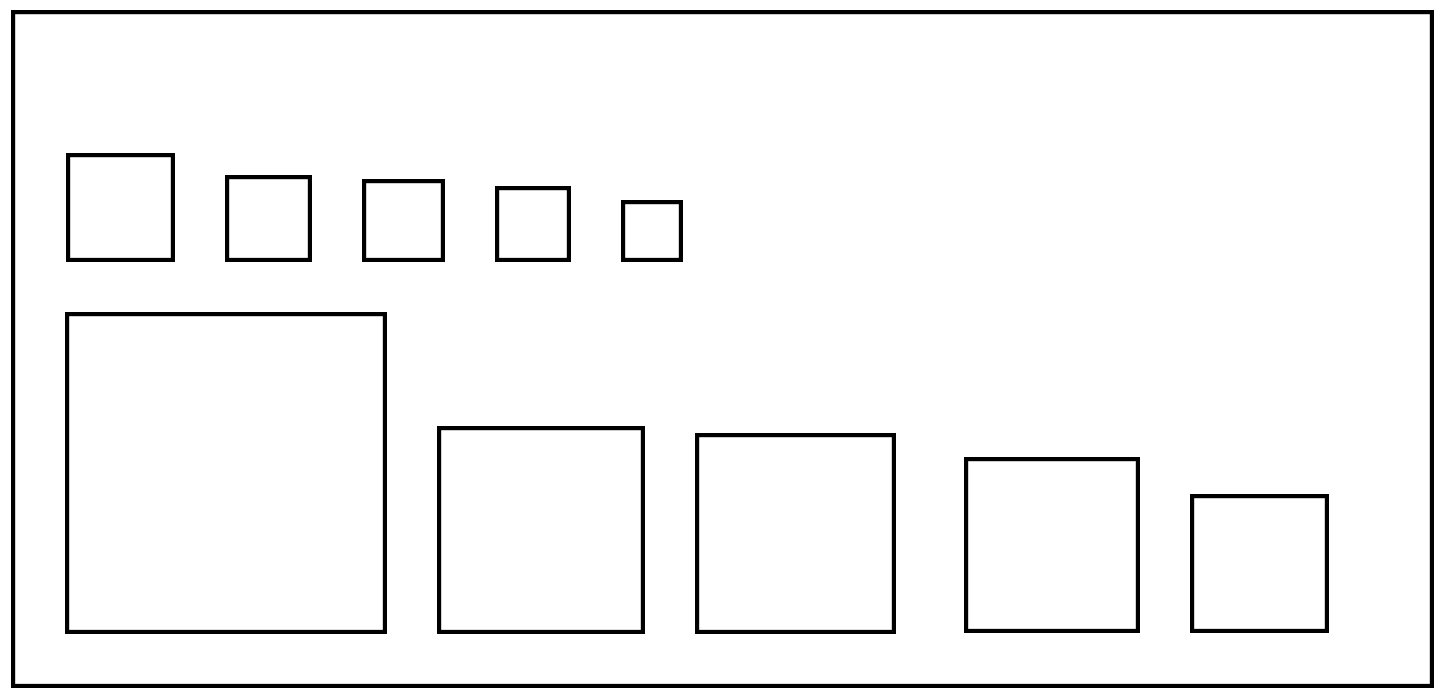
\includegraphics[width=.7\textwidth]{pictures/classPacking.png}
\caption{Explanation of how the classes are positioned in a package}
\label{fig:classesPacking}
\end{figure}


\subsubsection{Maximum packing} \label{Maximum packing}
Since in WebCity it is possible to dynamically change the version we are visualizing, it is important to maintain the position of the classes and packages that are present in multiple versions, so that the visualization remains coherent and familiar, and so that the different versions are comparable between each other.

To implement this, we first do the rectangle packing for each version of the system. When this is done, we collect the information of the packings and we merge them together into a final rectangle packing, called a maximum packing, where we consider all the packages and classes that existed in whole history of the repository, and if a package or class existed in multiple versions, then we make sure to consider its maximum size that it achieved during its evolution.
Then we can use this packing as a maximum possible dimension of the system, and we use it as a main rectangle packing for the visualization; when the user wants to change the version, we simply have to change the dimensions or the visibility of some package and classes, without having to move them around.

Figures \ref{fig:maxPacking} and \ref{fig:maxPacking2} show the maximum packing of the repository Apache Commons-math next to a normal version of the same repository. As we can see, the elements that exist in both representations have the same positions.


\begin{figure}[H]
  \centering
  \begin{minipage}[b]{0.49\textwidth}
      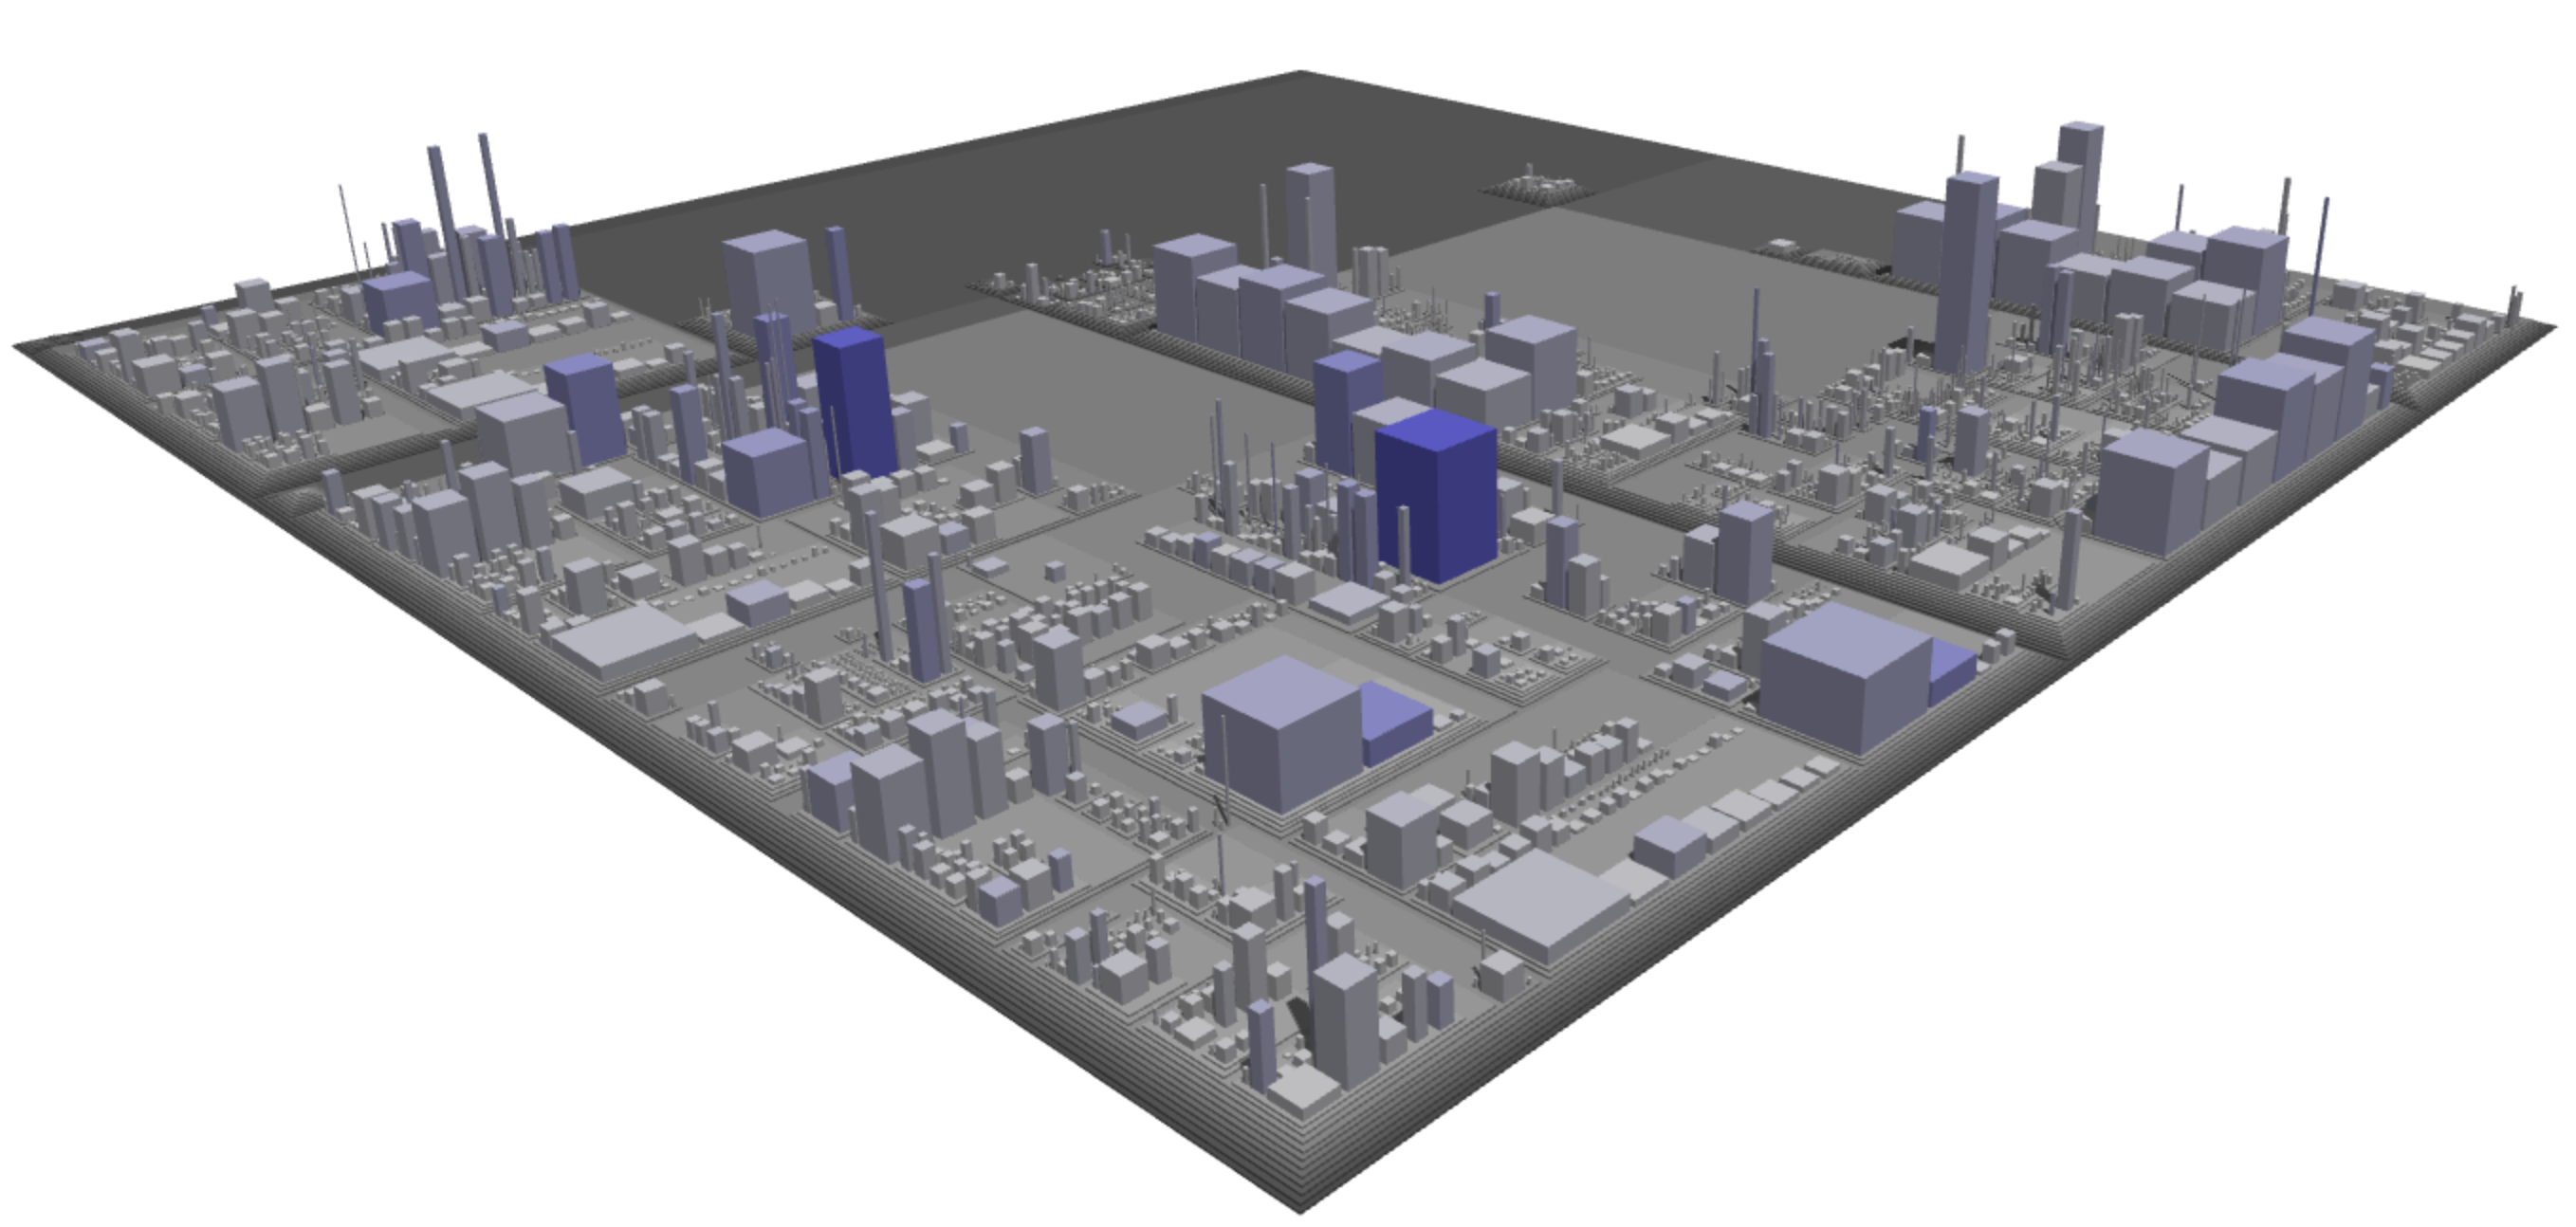
\includegraphics[width=1\textwidth]{pictures/maxDrawable1.png}
      \caption{The maximum packing of Apache Commons-math}
      \label{fig:maxPacking}
  \end{minipage}
  \hfill
  \begin{minipage}[b]{0.49\textwidth}
      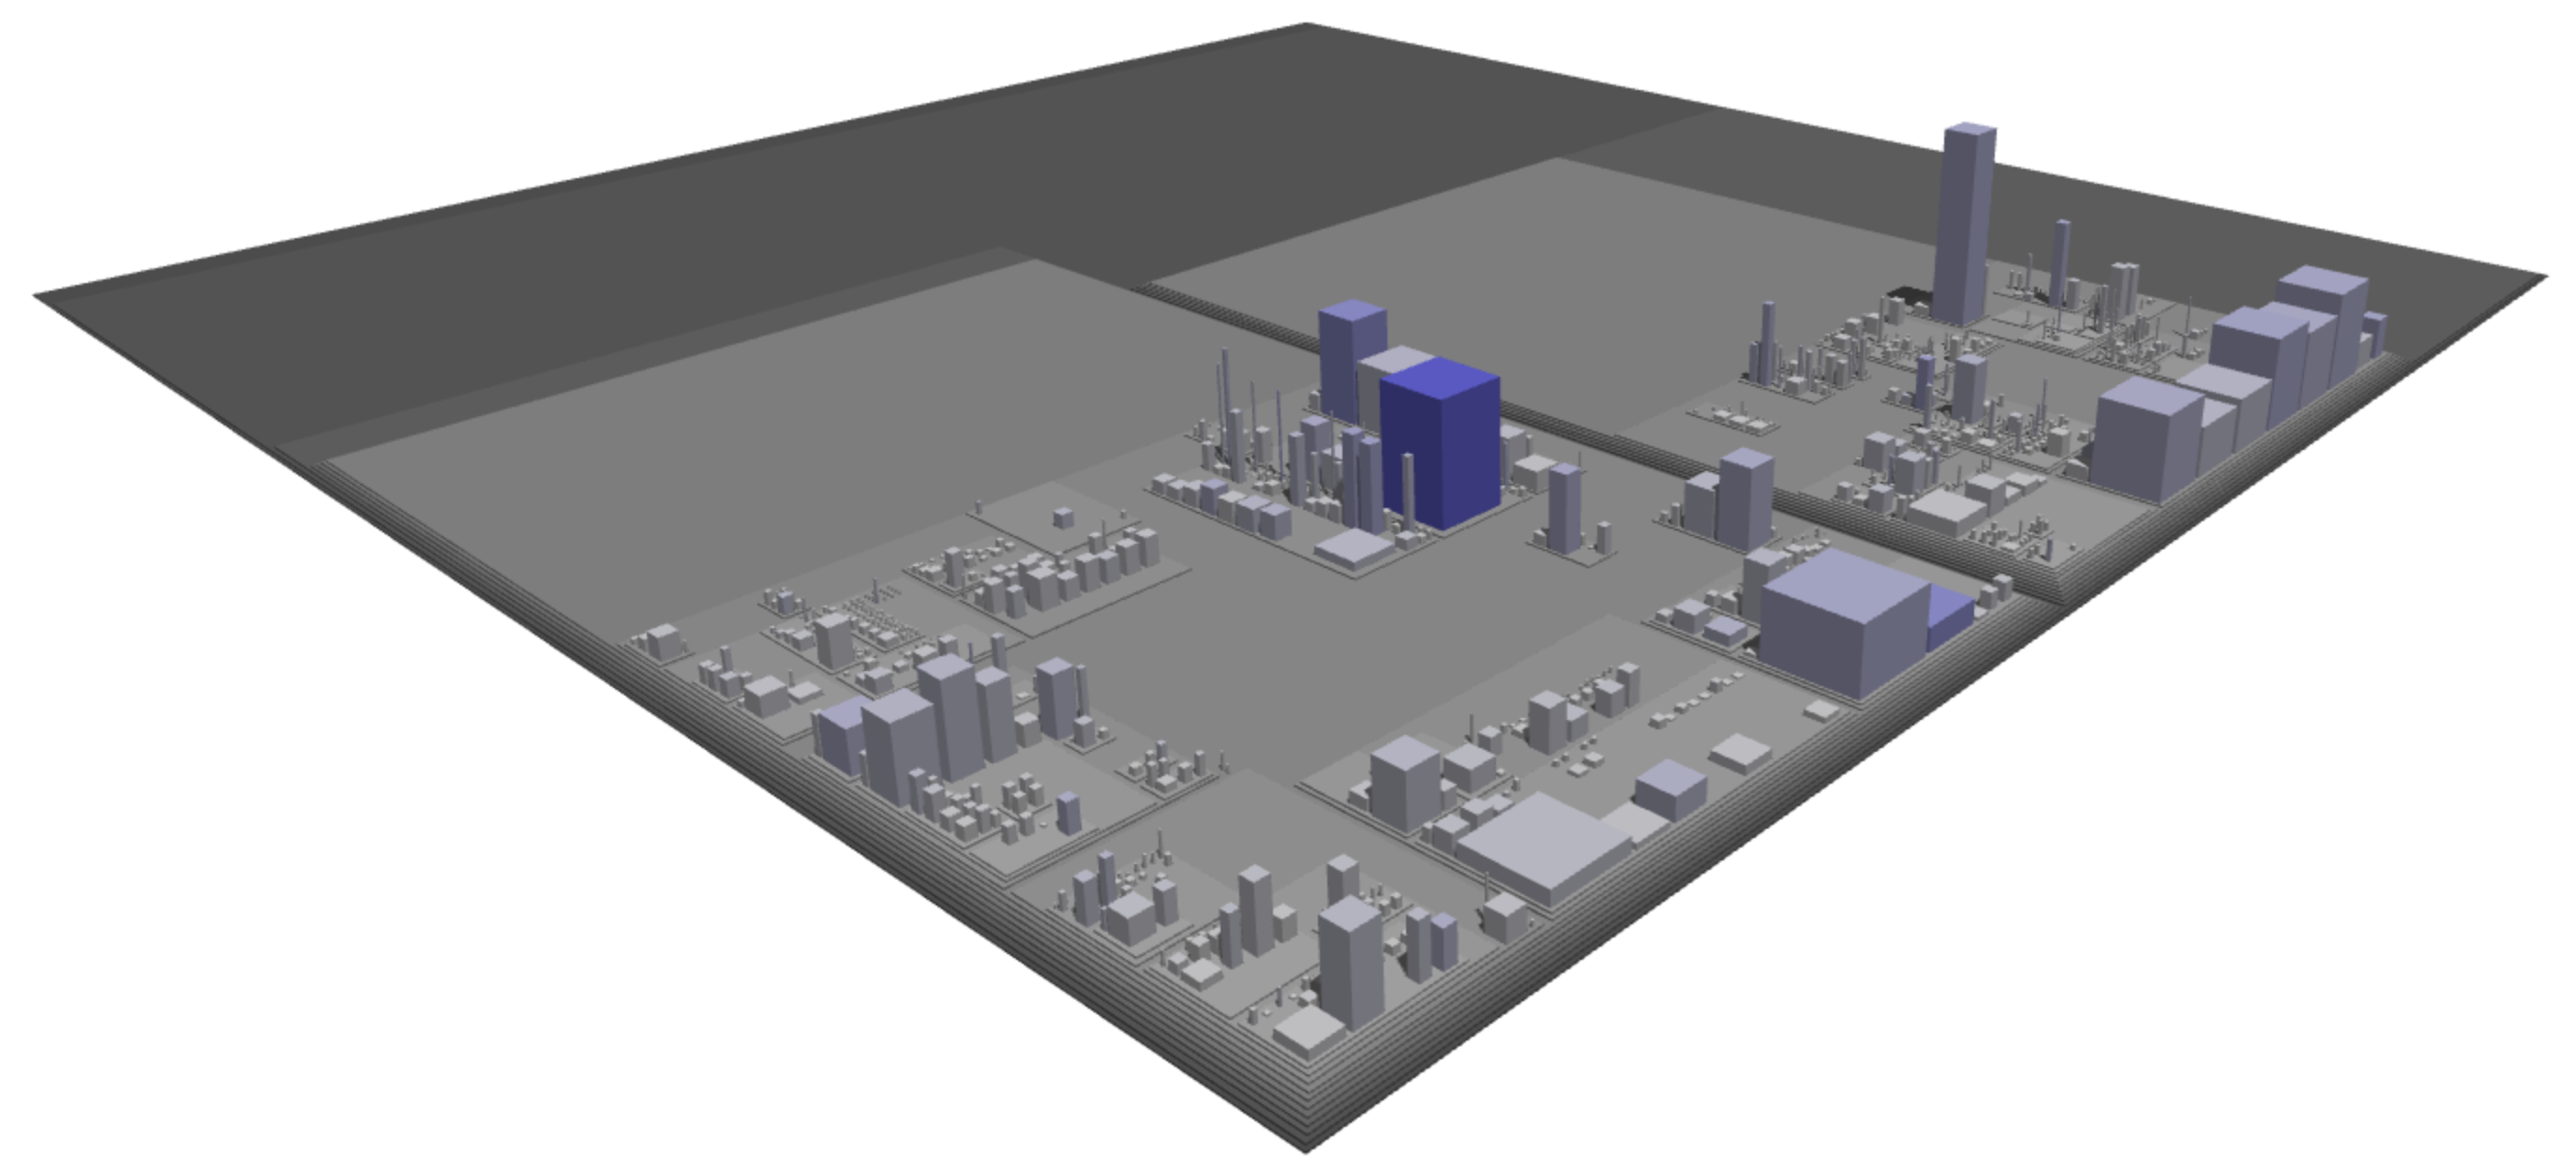
\includegraphics[width=1\textwidth]{pictures/maxDrawable2.png}
      \caption{A normal version of Apache Commons-math}
      \label{fig:maxPacking2}
  \end{minipage}
\end{figure}


\subsubsection{Visualizing the city} \label{Visualizing the city}
Once the rectangle packing is done, the data is sent back to the client, that has to set up the canvas for the visualization. This means creating a new canvas element, the lights, the controls to navigate the 3D space, the types and dimensions of shadows, the camera, and so on.
When this initialization part is done, we go through the list of drawable classes and packages that we received from the server. If a package is marked as visible it means that it exists in the current version, and therefore we have to draw the package itself and recursively its content. If instead it is marked as not visible, we do not draw the package and its content.

Both classes and packages are drawn on the canvas as simple boxes, with extra fields added, like its name, some information on the metrics, its type, and so on: these extra fields will be used for the interactive part, so that when we hover an object on the visualization, we already have all the information we need directly on the object itself.

Once we have created all the single meshes for the classes and the packages, we merge them into a single big mesh.
This is because if we were to keep them as different meshes, the performance would struggle when trying to move around thousands of different meshes at the same time. Since we know that the transformation that the objects go through is the same, we can merge the meshes into one big mesh, that represents the whole city.

%%%%%%%%%%%%%%%%%%%%%%%%%
\section{Results} \label{Results}
%%%%%%%%%%%%%%%%%%%%%%%%%

We will now present a short analysis of the general performance of the application, focusing on two main parts: the performance of the parsing and rectangle packing on the server side, and the video generation feature on the client side.

The parsing and packing will be tested by counting how long it takes to parse and pack different repositories with varying amounts of code and versions, while the video feature will be tested on a single repository, with different combination of settings.

\subsection{Visualization performance} \label{Visualization performance}

For the browser-based 3D visualization of the repositories we used Three.js, a Javascript library that allows users to interface with WebGL in a simpler and more straightforward way. WebGL is based on OpenGL ES 2.0, and even though it is not as mature as the latest versions of OpenGL and it lacks some of its features, it still provides solid performance while allowing to create and manipulate 3D graphics on the client side, allowing to draw directly onto HTML5 canvas elements.

While the first attempts turned out to be rather slow and laggy even with a small amount of objects being drawn on the canvas, with a couple of tricks and optimizations we were able to improve the performance, to the point where navigating and moving through the 3D visualization remains a quite smooth experience even when the number of objects is in the order of the thousands.

The first bottleneck was solved by merging all the meshes of the different objects, classes and packages, into a single very big mesh. This made the performance improve a lot, but this also takes away the possibility to have callbacks on the single elements, therefore making impossible to have hovering effects, classes highlighting and so on. This was solved by both having the single merged mesh alongside the list of single meshes. The meshes in the list are kept invisible, so that the performance is not impaired by them, but they still exist in the canvas, allowing to use them for ray-tracing intersections, and therefore have working callbacks and hovering events. Moreover, if we want to highlight an element, we can now simply find this element in the list of meshes and make it visible (and color it differently).

Another big performance improvement was obtained disabling the automatic update of the shadows, and manually telling the renderer to update them only when needed. This allowed us to have proper shadows and lighting without greatly affecting the performance.

Generating the visualization from scratch, when the repository contains many classes, packages and a big amount of versions to be parsed, can take a long time. We have analyzed the time it takes to generate the final visualization (where we have parsed every version of the repository's history) for different orders of magnitude. What takes most of the time is the actual parsing of the code, since we need to scan the code to gather the information for the metrics that will then be used for the visualization. The final part of generating the visualization when we already have the data takes only a small fraction of the total time.\\\\
We picked the following Java repositories to test the performance of the application:

\begin{itemize}
    \item https://github.com/AurecchiaP/webcity: our own repository on GitHub
    \item https://github.com/orbit/orbit: a framework to write distributed systems using virtual actors on the JVM
    \item https://github.com/javaparser/javaparser: a Java 1.0 to Java 9.0 Parser with AST generation and visitor support
    \item https://github.com/junit-team/junit4: a Java framework for unit testing
    \item https://github.com/google/ExoPlayer: a media player for Android systems
\end{itemize}

Table \ref{tab:performance2} contains information about the sizes of the repositories, and table \ref{tab:performance} shows the results of our tests.
Min. class number and Max. class number represent the lowest and highest amount of numbers found in any version of the repository,  and Min. LoC and Max. LoC represent the sum of the number of lines of code of the Java files in which the classes were found.

\begin{table}[H]
    \begin{center}
        \begin{tabular}{ | l | l | l | l | l | l |}
        \hline
        Repository & Min. class number & Max. class number & Min. LoC & Max. LoC \\ \hline
        WebCity & 6 & 45 & 52 & 3532 \\ \hline
        Orbit & 176 & 444 & 10344 & 25654 \\ \hline
        JavaParser & 130 & 558 & 21840 & 50158 \\ \hline
        Junit4 & 67 & 1159 & 4611 & 45073 \\ \hline
        ExoPlayer & 202 & 801 & 20192 & 109937 \\ \hline
        \end{tabular}
    \end{center}
    \caption{Sizes of the different repositories analyzed}
    \label{tab:performance2}
\end{table}

\begin{table}[H]
    \begin{center}
        \begin{tabular}{ | l | l | l | l | l | l |}
        \hline
        Repository & Versions & Parsing time & Generation time & Total time \\ \hline
        WebCity & 189 & 12s & <1s & 12s \\ \hline
        Orbit & 1536 & 370s & 4s & 374s \\ \hline
        JavaParser & 2238 & 424s & 2s & 426s \\ \hline
        Junit4 & 2448 & 464s & 3s & 467s \\ \hline
        ExoPlayer & 3568 & 1203s & 14s & 1217s \\ \hline
        \end{tabular}
    \end{center}
    \caption{Performance test on different repositories}
    \label{tab:performance}
\end{table}

As expected, both the number of elements to be parsed and the number of versions have an important influence on the time required to parse the history of a repository, while the generation time (mostly represented by the rectangle packing algorithm) is negligible.

\subsection{Video generation performance} \label{Video generation performance}
Tables \ref{tab:performance3} to \ref{tab:performance8} show some performance tests that we ran on the repository JavaParser, using different resolutions (720p, 1080p, 1440p), with different amount of versions (100, 250, 500, 1000, 2000), with and without orbit.

\begin{table}[H]
    \begin{center}
        \begin{tabular}{ | l | l | l | l | l | l |}
        \hline
        Versions & Screenshot time (s) & Generation time (s)& Total time (s) \\ \hline
        100 & 20 & 38 & 58 \\ \hline
        250 & 53 & 77 & 130 \\ \hline
        500 & 115 & 149 & 264\\ \hline
        1000 & 187 & 307 & 494 \\ \hline
        2000 & 293 & 542 & 835 \\ \hline
        \end{tabular}
    \end{center}
    \caption{720p, orbit}
    \label{tab:performance3}

    \begin{center}
        \begin{tabular}{ | l | l | l | l | l | l |}
        \hline
        Versions & Screenshot time (s) & Generation time (s)& Total time (s) \\ \hline
        100 & 20 & 39 & 59 \\ \hline
        250 & 50 & 45 & 95\\ \hline
        500 & 111 & 76 & 187\\ \hline
        1000 & 180 & 140 & 320 \\ \hline
        2000 & 286 & 274 & 560 \\ \hline
        \end{tabular}
    \end{center}
    \caption{720p, no orbit}
    \label{tab:performance4}

    \begin{center}
        \begin{tabular}{ | l | l | l | l | l | l |}
        \hline
        Versions & Screenshot time (s) & Generation time (s)& Total time (s) \\ \hline
        100 & 22 & 66 & 88 \\ \hline
        250 & 60 & 156 & 216\\ \hline
        500 & 128 & 433 & 561\\ \hline
        1000 & 197 & 637 & 834\\ \hline
        2000 & 323 & 1323 & 1646\\ \hline
        \end{tabular}
    \end{center}
    \caption{1080p, orbit}
    \label{tab:performance5}

    \begin{center}
        \begin{tabular}{ | l | l | l | l | l | l |}
        \hline
        Versions & Screenshot time (s) & Generation time (s)& Total time (s) \\ \hline
        100 & 21 & 41 & 62 \\ \hline
        250 & 58 & 104 & 162\\ \hline
        500 & 127 & 158 & 285\\ \hline
        1000 & 216 & 299 & 515\\ \hline
        2000 & 319 & 597 & 916\\ \hline
        \end{tabular}
    \end{center}
    \caption{1080p, no orbit}
    \label{tab:performance6}

    \begin{center}
        \begin{tabular}{ | l | l | l | l | l | l |}
        \hline
        Versions & Screenshot time (s) & Generation time (s)& Total time (s) \\ \hline
        100 & 25 & 107 & 132 \\ \hline
        250 & 69 & 255 & 324\\ \hline
        500 & 152 & 505 & 657\\ \hline
        1000 & 205 & 989 & 1194\\ \hline
        2000 & 437 & 1931 & 2398\\ \hline
        \end{tabular}
    \end{center}
    \caption{1440p, orbit}
    \label{tab:performance7}
    \end{table}

\begin{table}[H]
    \begin{center}
        \begin{tabular}{ | l | l | l | l | l | l |}
        \hline
        Versions & Screenshot time (s) & Generation time (s)& Total time (s) \\ \hline
        100 & 25 & 64 & 89 \\ \hline
        250 & 69 & 137 & 206\\ \hline
        500 & 155 & 266 & 421\\ \hline
        1000 & 204 & 526 & 730\\ \hline
        2000 & 436 & 1050 & 1516\\ \hline
        \end{tabular}
    \end{center}
    \caption{1440p, no orbit}
    \label{tab:performance8}
\end{table}

Figure \ref{fig:plot} shows a plot of the performance results with the different video settings:

\begin{figure} [H]
\centering
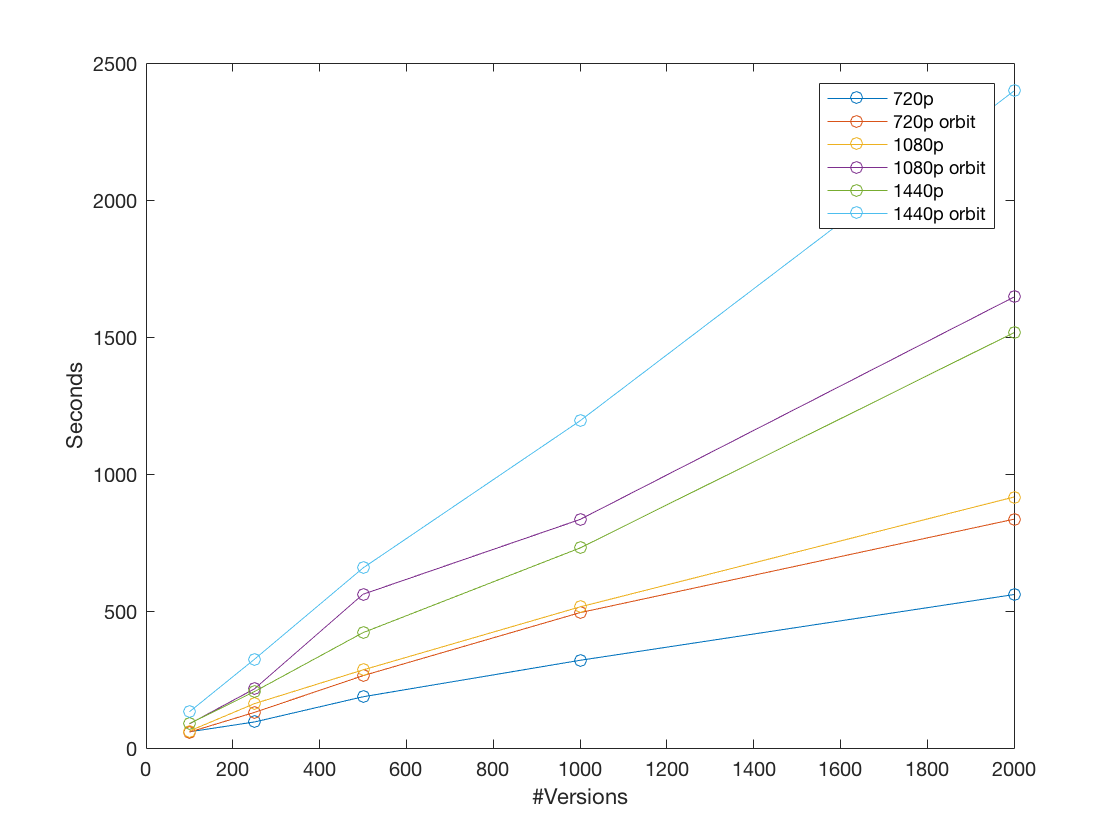
\includegraphics[width=1\textwidth]{pictures/figure1.png}
\caption{Comparison of the video generation performance}
\label{fig:plot}
\end{figure}

As we can see from the results, we can notice how the videos generated with the orbit option take almost twice as much time
as the ones without orbit. This is because when we are not orbiting, there's a higher chance for pixels not to change between multiple screenshots, which means that there's less data to handle and the generation takes less time.
Also, as expected, increasing the resolution also increases the generation time: from what we can see, changing to a higher resolution increases the total time by around 50\%.

\subsubsection{Implementation issues} \label{Implementation issues}

The video generation feature is implemented almost completely on the client side. This is because to be able to do this on the server side we would have had to also be able to create the visualizations on the server side, which, without changing our current architecture, is not possible: Three.js, the library used to create the 3D cities, is a strictly web focused library. To be able to use it on the server we then would need a way to build a second web app on the server, which most likely means changing the whole server side.




%%%%%%%%%%%%%%%%%%%%%%%%%
\section{Conclusions} \label{Conclusions and future work}
%%%%%%%%%%%%%%%%%%%%%%%%%
We presented WebCity, a browser-based application that was inspired by the work on software visualization that was done previously \cite{Wett07b} \cite{Wett2008b} \cite{Wett2008a} in a user-friendly platform, while also expanding it with other features.
We presented the data with the model of the city, that aims at improving and simplifying the usability of the system.
We implemented various features, like display of element information on hover, search and tagging of elements, visualization of source code, free 3D navigation that includes pitch, yaw, pan and zoom, navigation of versions and video generation of the history of a repository.

For the future work on WebCity, it would be interesting to further improve the amount of features provided to the user for navigating and analysing the visualization, and perhaps finding new or alternative ways to increase the number of metrics and general information displayed about the system.
Some work could also involve the performance, aiming at reducing the waiting time for the setup of the visualization and the generation of videos for big and historically complex repositories, improving the scalability of the application.

It would also be interesting to broaden the number of supported languages. At the moment, only the analysis of Java based repositories is available: in the future support for other languages could be added, with perhaps different visualizations or by creating a single visualization that shows classes and packages of different languages and the relationships between them.


% \subsection{General issues}
%
% Latex is not so complex. If you aren't familiar with it just spend some time in googling for latex commands (e.g. font formats, tables, figures, items,\dots).
%
% \subsection{Getting started}
% In order to use the bachelor thesis template, be sure that the following files are present in your working directory:
% \begin{itemize}
% \item usiinfbachelorproject.cls (The latex template)
% \item logo-info.pdf (The logo figure)
% \item references.bib (The references file)\\
% \end{itemize}
%
% \subsection {Compilation issues}
%
% If you are not familiar with Tex, I advise you to download TexShop for Mac OS.\\
% To include the references and display them in the final pdf, you have first to typeset this file with \textit{LaTex} (ComboBox upper left, if you use TexShop), then with \textit{BibTex} and finally again with \textit{LaTex}.\\
% In order to resolve figures/table/\dots~references you have to run 2 times the (latex) typeset.
%
% \subsection {Document structure}
%
% Some basic sections:
% \begin{itemize}
% \item Introduction (including Motivation)
% \item State of the Art
% \item Project requirements and analysis
% \item Project design (top-down)
% \item Implementation issues (bottom-up)
% \item Tests (methodology, results, comments)
% \item Conclusions and future work or possible developments
% \end{itemize}
%
% \subsection {Some examples}
%
% \textbf{Figure ~\ref{fig:USILogo}} shows how to insert figures in the document.
%
% \begin{figure} [H]
% \centering
% 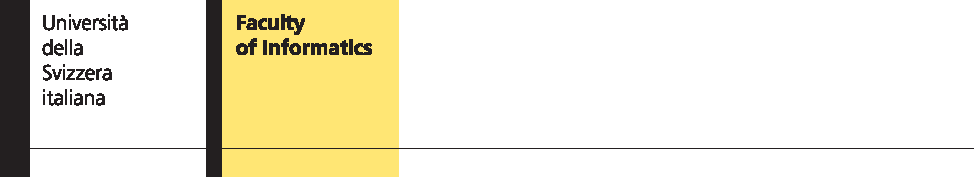
\includegraphics[width=0.5\textwidth]{logo-info.pdf}
% \caption{Caption of the figure}
% \label{fig:USILogo}
% \end{figure}
%
% \noindent\textbf{Table ~\ref{tab:numbers}} shows how to insert tables in the document.
%
% \begin{table}[H]
% \centering
% \scalebox {0.8} {
% \begin{normalsize}\begin{tabular}{l|lll}
% \textbf{Col 1} & \textbf{Col 2} & \textbf{Col 3} & \textbf{Col 4}\\
% \hline
% 1 & 2 & 3 & Goofy\\
% 4 & 5 & 6 & Mickey
% \end{tabular}
% \end{normalsize}
% }
% \caption{Caption of the table}
% \label{tab:numbers}
% \end{table}



%%%%%
\newpage
\bibliographystyle{abbrv}
\bibliography{references}

\end{document}
